\documentclass[reprint,amsmath,amssymb,aps,pre,showkeys,showpacs]{revtex4-1}
% Latex
\usepackage[english]{babel}
\usepackage[utf8]{inputenc}
\usepackage[T1]{fontenc}
% Xelatex
%\usepackage{polyglossia}
%\usepackage{fontspec}
%\setdefaultlanguage{english}
%\setmainfont{DejaVu Sans}
%\setsansfont{DejaVu Sans}
%\setmonofont{DejaVu Sans Mono}
\usepackage{bm}
\usepackage{cleveref}
\usepackage{xcolor}
\usepackage{algpseudocode}
\usepackage{graphicx}
\usepackage{subfigure}

\definecolor{light-gray}{gray}{0.95}
\newcommand{\code}[1]{\colorbox{light-gray}{\texttt{#1}}}
% When cleveref fails to do its job
\newcommand{\apref}[1]{Appendix \ref{#1}}

\begin{document}
\preprint{APS/123-QED}

\author{Aleksei I. Samarin\textsuperscript{1,2}}
\author{Vasily Postnicov\textsuperscript{1}}
\author{Marina V. Karsanina\textsuperscript{1}}
\author{Efim V. Lavrukhin\textsuperscript{1,2}}
\author{Alexey N. Khlyupin\textsuperscript{1,3}}
\author{Kirill M. Gerke\textsuperscript{1}}
\email{kg@ifz.ru}

\affiliation{\textsuperscript{1}Schmidt Institute of Physics of the Earth of
  Russian Academy of Sciences, Moscow, 107031, Russia}
\affiliation{\textsuperscript{2}Computational Mathematics and Cybernetics,
  Lomonosov Moscow State University, Moscow, 119991, Russia}
\affiliation{\textsuperscript{3}Moscow Institute of Physics and Technology, 9
  Institutskiy per., Dolgoprudny, Moscow Region, 141701, Russia}

\title{Robust surface correlation functions evaluation from experimental
  discrete digital images}

\begin{abstract}
  Pore-scale modelling based on the 3D structural information of porous
  materials has enournous potential in assessing physical properties beyond the
  capabilities of laboratiry methods. Such capabilities are pricely in terms of
  computational expenses - this limits the applicability of the direct
  simulations to a small volume and requires high performance computational
  resources, espeically for multi-phase flow simulations. The only pore-scale
  technique capable of dealing with large representative volumes of porous
  samples is pore-network (PNM) based modelling. The problem of PNM approach is
  that 3D pore geometry first needs to be simplified into a graph of pores and
  throats that conserve topological and geometrical properties of the original
  3D image. While a lot of progress was achieved in terms of geometry
  representation, no methodology provides full conservation of the topological
  features of the pore structure.  In this paper we present a pore-network
  extraction algorithm for binary 3D images based on discrete Morse theory and
  persistent homology that by design targets topology preservation. In addition
  to methdological developments, we also clarify the relationship between
  topological characteristics of constructed Morse chain complex and
  pore-network elements. We show, that the Euler numbers calculated for PNMs
  based on our methodology coincide with those obtained using the direct
  topological analysis. The characteristics of extracted pore-network are
  calculated for several 3D porous binary images and compared with the results
  of maximum inscribed balls-based, watershed-based and hybrid approach to
  support our methdology.
\end{abstract}
\keywords {3D images; correlation functions; surface-surface function;
  surface-void function; image analysis; image scaling}

\maketitle

\section{Introduction}
Correlation functions (CFs) are invaluable universal descriptors of structure
and in this context are utilized in a multitude of scientific disciplines:
material sciences \cite{Cecen,chen2022quantifying}, rock
\cite{ledesma2018effect} and soil physics
\cite{Euras2012,PLoS_ONE,KarsaninaEJSS}, cosmology \cite{TakadaJain} and food
engineering \cite{Derossi2019}, to name just a handful. As such, CFs were used
to characterize the morphology \cite{tensorPRE} and representativeness via
correlation lengths \cite{vcapek2011transport,thovert2011grain}, compare
structures \cite{jiao2014chawla,EPL1,REVpaper}, compress structural information
\cite{SciRep1,Havelka,KarsaninaEJSS}, describe structural dynamics
\cite{chen2015dynamic,PLoS_ONE,xu2022correlation}, extract features for deep
learning \cite{Miao2017,kamrava2020linking,roding2020predicting,KarsaninaEJSS},
perform stochastic reconstructions
\cite{Adler_recon,Y-T,EPL2,tahmasebiPRL,karsaninaPRL} and fuse multi-scale
images \cite{SciRep1,chen2016stochastic,Geoderma2018}. Stochastic reconstruction
is a special topic of interest, as this approach allows to solve an inverse
problem and recover structure from a known set of correlation functions –- and
this ability for recovery is the basis for majority of potential usages in the
list above. Early reconstruction techniques mainly involved two-point
probability $S_2$ function, but were improved to include lineal $L_2$ function
\cite{Y-T,vcapek2009stochastic,vcapek2011transport}, cluster $C_2$ function
\cite{JiaoPNAS,jiao2014chawla} and potentially surface-surface $F_{ss}$
function. With the proper handling \cite{EPL2} it is possible to incorporate
numerous CFs into a reconstruction procedure. Increasing the number (and order)
of functions leads to higher information content of the CFs set
\cite{Gommes1,Gommes2}, thus, it allows to reconstruct and perform
stationarity/representativeness characterization \cite{REVpaper} for structures
of any complexity.

There are two ways to obtain correlation functions for a given structure at hand
-- either measure them experimentally with the help of scattering intensity
\cite{debye1957scattering,li2018accurate}, or measured from images. The first
approach suffers from the limitation of CFs that can be obtained this way
\cite{Gommes_notchord}, while the second one provides information with limited
resolution or/and resolution to field-of-view ratio \cite{SciRep1}. Moreover,
the most useful imaging methods such as X-ray computed tomography (XCT) and
scanning electron microscopy (SEM) due to their underlying physical principles
provide gray-scale images which, as we shall argue later on, need to be
segmented into constituent phases before CFs computation. It is important to
note that such gray-scale images do not represent spatial distribution of the
phases, but, for example, X-ray spatial attenuation or electron back-scattering
intensities. However, if properly segmented, high-resolution digital images do
provide a possibility to compute any correlation function. Experimental
measurements using small angle scattering (SAS) are traditionally used to
evaluate $S_2$, but it is also possible to relate scattering intensities to
surface correlation functions \cite{dietrich1995scattering,ma2018SS}. It would
be of great practical importance to obtain surface correlation functions from
both SAS and imaging (focused ion beam milling combined with SEM allows to
obtain the finest imaging resolutions comparable to SAS and sample CFs from
polished surfaces as opposed to surface imaging \cite{FIB-SEMpaper}) to estimate
coefficients for surface and bulk scattering (see Eq.13 in \cite{ma2018SS}). But
there is a catch -- SAS possesses close to infinite surface resolution as
opposed to digital pixelized images with inherent segmentation problems due to
partial volume effects, something we discuss next.

Recently, Ma and Torquato \cite{ma2018SS} laid foundation to precise surface
correlation function computations and showed the usefulness of these CFs
evaluation for numerous problems. They have implemented an elegant solution with
the help of infinite resolution random fields that allows finding an exact
intersection with the sampling line. In addition, they also showed that surface
CFs for digital images can be computed by converting integer fields (i.e.,
location of the phases) to float fields with the help of Gaussian filter
\cite{ma2018SS}. Unfortunately, their solution is not readily applicable to the
majority of grey-scale images due to non-singularity in their chemical
constitution. The reason is the difference between the contour and real
interface between different phases within the material due to the partial volume
effects \cite{Wildenschild_Sheppard} for XCT imaging -- the presence of multiple
phases within the same pixel/voxel. In other words, the attenuation is a
function of both density and atomic number, which usually are distributed
non-uniformly below the XCT imaging resolution. Somewhat similar is also
relevant for SEM imaging, as secondary or back-scattered electrons are
effectively a convolution of partial signals coming from different depths
\cite{Bultreys_review}. The exact sub-voxel thresholding based on gray-scale
image (similar to the technique used in \cite{ma2018SS}) is only available in
case it is monomineral, i.~e., the solid phase consists of a completely
chemically homogeneous substance that contrasts perfectly with air/vacuum filled
pore phase -- this is rarely the case for natural materials. Moreover, even if
the image of a monomineral sample has sub-resolution features on XCT image,
while it is possible to compute the porosity of the voxel, it's still not
possible to extract the interface. All these and additional problems (such as,
for example, experimental noise and artifacts from inverse Radon transform)
arising during gray-scale image processing as related to image segmentation were
extensively discussed elsewhere \cite{NNseg}. In other words, simple
thresholding of the grey-scale image to compute surface functions using the
approach proposed in \cite{ma2018SS} (their section V.C) may result in incorrect
surface identification and surface functions are not defined for grey-scale
images (due to possible sub-resolution porosity). Thus, we argue, that the usage
of current state-of-the-art segmentation techniques is necessary prior to the
conversiton to a coarse-grained scalar field. Moreover, finding an intersection
between a line segment and the countour is a computationally expensive procedure
that prevents on-the-fly application of surface functions. If a binary image
(consisting of pores and solids) is produced by adequate segmentation technique,
we still lack a robust and computationally effective procedure to evaluate
surface CFs from experimental XCT and SEM images of natural heterogeneous
materials, for instance, rocks and soils.

\begin{figure}[ht]
  \centering
  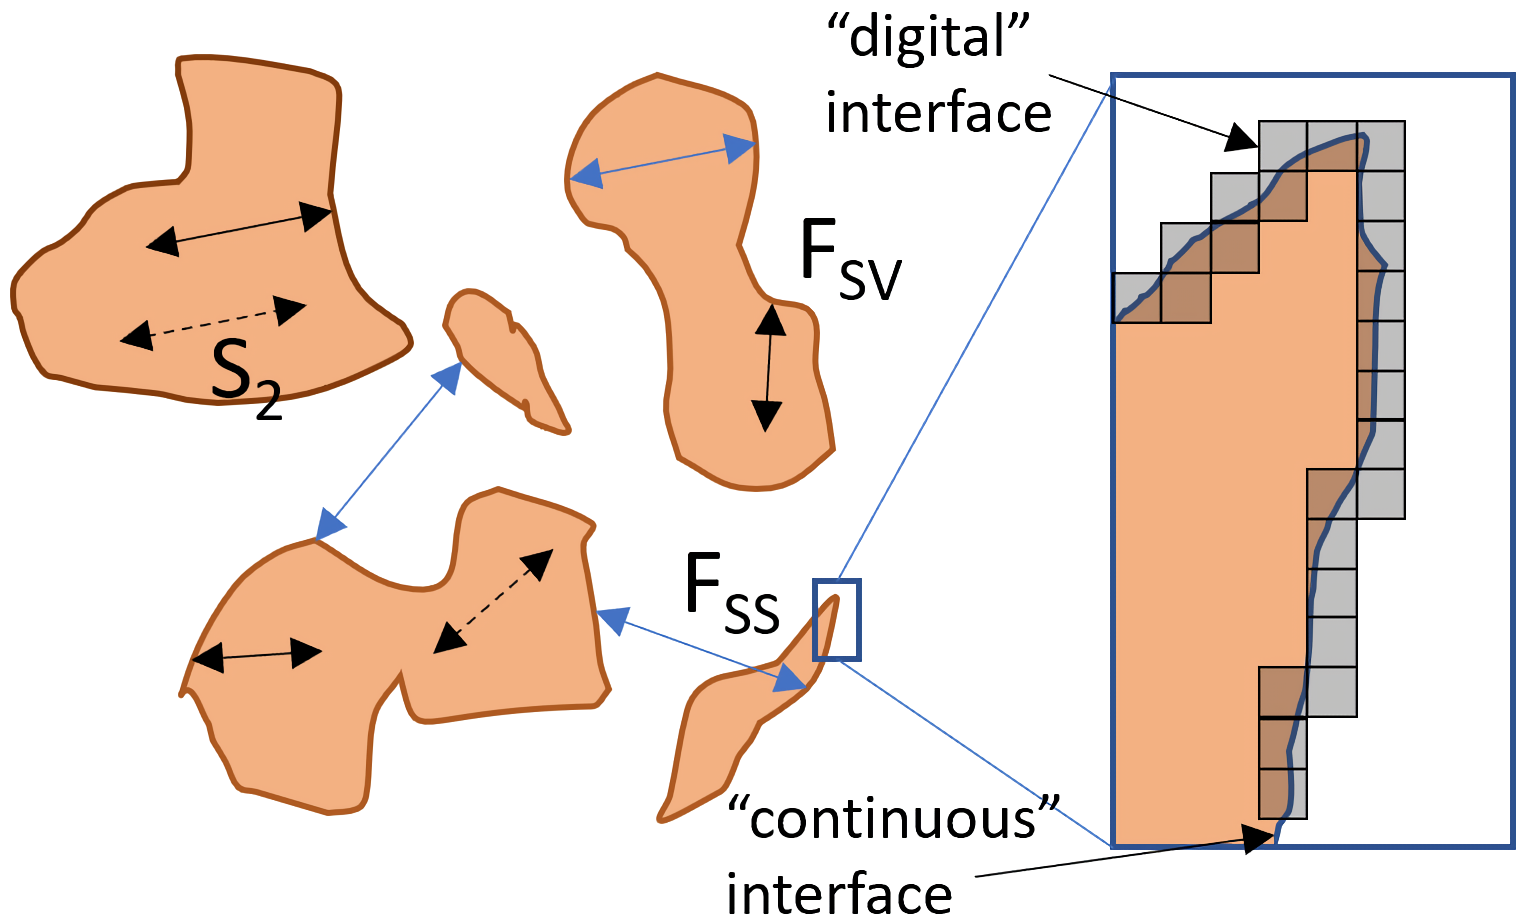
\includegraphics[width=0.9\linewidth]{images/scheme.png}
  \caption[]{A schematic depiction of a binary porous media (pores are shown in
    color) with examples of positive events for surface $F_{ss}$, $F_{sv}$ and
    two-point probability $S_2$ correlation functions. The zoomed in area
    represents the difference between the true ``continuous'' interface in
    between pore and solid phases with pixelized ``digital'' interface emerging
    due to limited resolution of digital images.}
  \label{fig:scheme}
\end{figure}

To compute surface functions one first needs to elucidate the interface between
two phases (we shall consider only pores and solids, but, obviously, the
computations can be perfromed to multi-phase systems in the similar manner). The
interface area has infinitesimal volume, but its location on the digital image
is not easy due to the pixelization of the interface between the binary phases
\cite{ma2018SS}. By adopting the $\varepsilon$ = pixel/voxel size one can create
a very crude approximation of the real interface, but the usage of interfaces
between voxels ``as is'' leads to known problems in surface area and surface
geometry evaluation, in application of 3D imaging for geometry and topology
analysis \cite{AWR_PNM} or energy minimization problems
\cite{frank2018energy}. Another option would be to describe the boundaries
between voxels with some curves, e.~g., splines. This way it would be possible
to perform surface CFs sampling by line intersection as described by Ma and
Torquato \cite{ma2018SS}. While an exact boundary can be obtained for
deterministic structures such as disk/sphere packings, splines would provide
only a very approximate solution for the boundaries of arbitrary digitized
structure due to the limit in resolution for a given image
\cite{gerke2012tomographic}. In other words, contours extracted from digital
images will approach real boundaries between phases only when the spatial
resolution approaches infinity. But the same is also true for digital
pixelized/voxelized images. Thus, the options to compute surface correlation
functions include ``continuous'' approach (such as implemented in
\cite{ma2018SS}) and ``digital'' approach (similar to computation of $S_2$ from
digital images) as depicted in \cref{fig:scheme}. Here we propose a modified
``digital'' approach that lies in between the exact and pixelized solutions for
a number of reasons:
\begin{enumerate}
  \item For a binarized XCT or SEM image the interpolation of the interface
    using "continuous" or "digital" in the limit of $\varepsilon \to 0$ would
    produce the same results. Thus, as it is not possible to obtain the exact
    continuous interface from such an image, using "digital" approach is natural
    as applied to digital pixel/voxel images.
  \item Continuous approach is expensive numerically, as it requires to find the
    intersections between a line and a curve.
  \item Digital approach allows to utilize linear scan CFs computation or with
    the usage of the Fast Fourier Transform (FFT) - the latter is a fastest way
    to evaluate full CFs map and very efficient on modern GPUs.
\end{enumerate}

In this paper we build upon foundational work of Ma and Torquato \cite{ma2018SS}
and develop a robust and efficient approach to compute surface correlation
functions from digital 2D and 3D images. The rest of the manuscript is organized
as follows: in \cref{sec:details} we provide all methodological details for
surface CFs computation including analytical solutions to verify the proposed
methodology and describe an image library for extensive testing of our
algorithms, \cref{sec:results} presents all major results of surface functions
evaluations. We discuss obtained results, including the effects of image
scaling, and outline future uses of surface functions within
\cref{sec:outline}. The paper concludes with a summary in \cref{sec:summary}.

\section{Theoretical background}
\label{sec:theory}
\subsection{Correlation functions and definitions}
\label{sec:definitions}
Firstly, we introduce an indicator function $I^{(i)}(\mathbf{x})$ which marks
pixels of 2D and voxels of 3D digitized images as belonging to the phase $i$ or
not. It can be defined so:
\begin{equation*}
  I^{(i)}(\mathbf{x}) = \left\{
  \begin{array}{ll}
    1 & \quad \mathbf{x} \in V_i \\
    0 & \quad \text{otherwise}
  \end{array}
  \right.
\end{equation*}
where $V_i \subset \mathbb{R}^n$ is the region occupied by phase $i$. For
statistically homogeneous media the ensemble average of $I^{(i)}$ equals volume
fraction of a given phase. For binary media the following equality holds:
\begin{align*}
  \phi_{void} &+ \phi_{solid} = 1 \\
  \phi_i &= \langle I^{(i)}(\mathbf{x}) \rangle
\end{align*}
In a similar fashion we can define an interface indicator function
$M(\mathbf{x})$ which provides interface area $s$ if averaged over the whole
image:
\begin{align}
  M(\mathbf{x}) = |\nabla I^{(solid)}(\mathbf{x})| &= |\nabla I^{(void)}(\mathbf{x})|
  \label{eq:interface} \\
  \langle M(\mathbf{x}) \rangle &= s
  \label{eq:surface}
\end{align}
The simplest, yet foundational correlation function is the two-point probability
function $S_2$ which is defined as a probability that the ends of a random line
segment belong to the same phase:
\begin{equation}
  S_2^{(i)}(\mathbf{x}_1, \mathbf{x}_2) = \langle I^{(i)}(\mathbf{x}_1)
  I^{(i)}(\mathbf{x}_2) \rangle \label{eq:twopoint}
\end{equation}
This equation can be further simplified for statistically homogeneous media, as
$S_2$ will dependent only on the relative displacement $\mathbf{r}$:
\begin{equation*}
  S_2^{(i)}(\mathbf{x}_1, \mathbf{x}_2) = S_2^{(i)}(\mathbf{r})
\end{equation*}
The value of $S^{(i)}_2(\mathbf{r})$ at $\mathbf{r} = 0$ is a fraction of phase
$i$ in a medium:
\begin{equation*}
  S_2^{(i)}(0) = \phi_i
\end{equation*}
For isotropic media a vector displacement $\mathbf{r}$ can be replaced with its
length $r = |\mathbf{r}|$ and $S_2(\mathbf{r})$ with $S_2(r) = S_2(|\mathbf{r}|)$.
Now, analogously to $S_2$ we can define surface-surface and surface-void
correlation functions (for homogeneous and isotropic media straight away):
\begin{align}
  F_{ss}(r) &= \langle M(x)M(x+r) \rangle \label{eq:fss} \\
  F_{sv}(r) &= \langle M(x)I^{(void)}(x+r) \label{eq:fsv} \rangle
\end{align}

The interface indicator function $M(x)$ is basically defined as infinity on the
interface and zero elsewhere. Therefore, it is hard to directly compute
$\langle M(x), M(x + r) \rangle$. We can replace the line of zero width and infinite value
with a strip of width $\varepsilon$ and value $\frac{1}{\varepsilon}$: $M(x; \varepsilon)$.
Then $F_{ss}(x; \varepsilon) = \langle M(x; \varepsilon), M(x + r; \varepsilon) \rangle$
is simply an intersection area of two strips -- original and shifted --
multiplied by $(\frac{1}{\varepsilon})^2$.
And with $\varepsilon \to 0 \Rightarrow F_{ss}(r; \varepsilon) \to F_{ss}(r)$.
Area between two black dashed circles on \cref{fig:Fss-explained} represents
$M(x; \varepsilon)$, red is for $M(x + r; \varepsilon)$. Blue color marks the
intersection area. More detailed information on two-point probability and
surface correlation functions can be found in comprehensive Torquato's book
\cite{Torquato_book}.

\begin{figure}
  \centering
  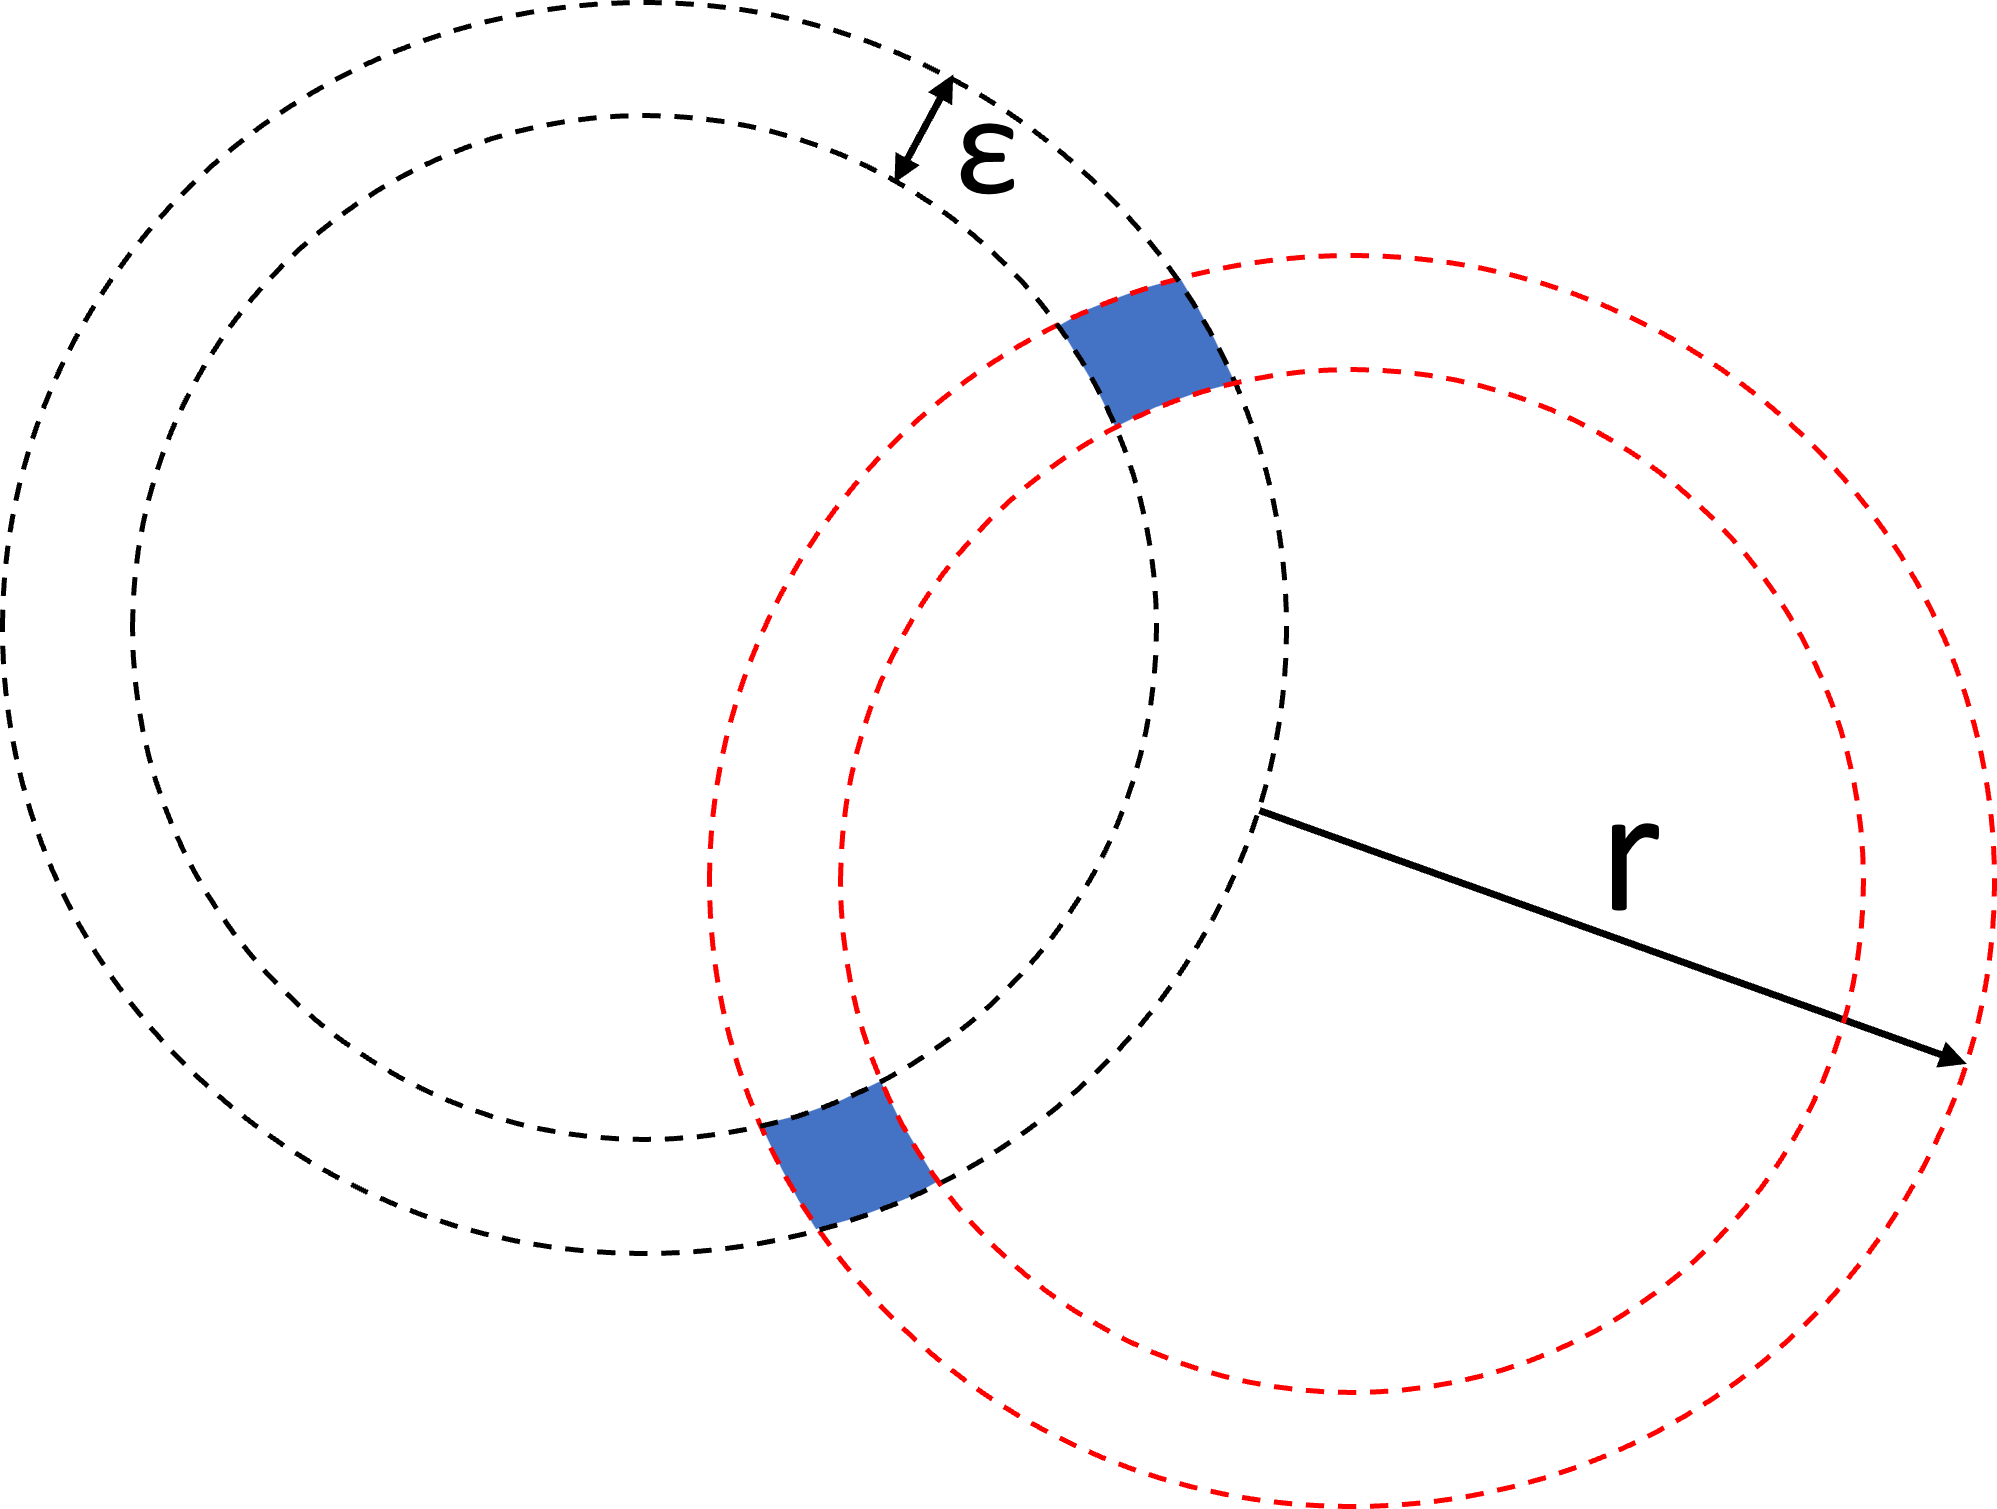
\includegraphics[width=0.9\linewidth]{images/Fss.png}
  \caption[]{Interpretation of $F_{ss}$ as self-intersection of the interface.
    \textcolor{red}{Torquato described it as ``previous algorithm'', fig.3 - actually not, their case is different a bit in my opinion (Kirill), let's discuss}}
  \label{fig:Fss-explained}
\end{figure}

\subsection{Analytical solutions}
For Poisson disks and spheres one can derive exact analytical surface-surface and
surface-void functions. For overlapping disks with radius $R$ and centers
generated by Poisson point process with parameter $\lambda$ we have (see the
derivation of these formulas in \cref{ap:overlapping-disks}):
\begin{align}
  F_{sv}(r) &= S_2(r) \left\{
  \begin{array}{ll}
    2(\pi - B)R \lambda & \quad r<2R \\
    2\pi R \lambda & \quad \text{otherwise}
  \end{array} \right. \label{eq:fsv_final} \\
  F_{ss}(r) &= S_2(r) \left\{
  \begin{array}{ll}
    \frac{(2(B-\pi)R\lambda)^2Ar + 4\sqrt{A}R^2\lambda}{Ar} & \quad r<2R \\
    (2\pi R\lambda)^2 & \quad \text{otherwise},
  \end{array} \right. \label{eq:fss_final}
\end{align}
where $S_2$ is the regular two-point correlation function and
\begin{align*}
  A &= 4R^2 - r^2 \\
  B &= \arccos(\frac{r}{2R}).
\end{align*}

For 3D balls the relationships are readily available in the literature
\cite{Torquato_book,ma2018SS}:
\begin{align*}
  F_{sv}(r) &= S_2(r) \left\{
  \begin{array}{ll}
    4\pi R^2\lambda(\frac{1}{2} + \frac{r}{4R}) & \quad r<2R \\
    4\pi R^2\lambda & \quad \text{otherwise}
  \end{array} \right. \\
  F_{ss}(r) &= S_2(r) \left\{
  \begin{array}{ll}
    {(4\pi R^2 \lambda (\frac{1}{2} + \frac{r}{4R}))^2 + \frac{2\pi R^2 \lambda}{r}} & \quad r<2R \\
    (4\pi R^2 \lambda)^2 & \quad \text{otherwise}.
  \end{array} \right.
\end{align*}

These analytical solutions will be used to verify the accuracy of our evaluation
of surface CFs for such systems.

\section{Methodological details}
\label{sec:details}
By looking at \cref{eq:twopoint,eq:fss,eq:fsv} one can observe
some significant similarities between two-point probability and two-point
surface functions (see \cref{fig:scheme}). The $S_2$ can be viewed as a
autocorrelation of the image, i.~e., computing correlations between shifted
realization of the image -- something that can be used to effectively compute
$S_2$ with the help of the FFT on modern hardware, especially GPUs. If we apply
the same analogy to $F_{ss}$, \cref{eq:fss} can be considered as an intersection
of the interface with itself for all possible shifts. Recall that for the
correlation length of zero this intersection is technically infinity
(\cref{sec:definitions}). While surface-void function is well defined at $r=0$,
it differs from $S_2$ in two significant aspects. First, it resembles two-point
cross-correlation function (as instead of autocorrelation we have to compute
correlation between the interface and the void phase). Second, such
cross-correlation is not commutative, so we get two surface-void functions:
correlation between an interface and a void phase and correlation between a void
phase and an interface. These considerations will be very useful in
understanding of our computational framework as described in this section.

\subsection{The general algorithm}
\label{sec:general}
While we present and compare a bunch of sligtly different methods to evaluate
surface CFs, they are all based on a single general algorithm for each surface
function as desribed below ($A$ refers to the input 2D or 3D digital image, $M$
is the interface between two phases, and $V$ is the image of the void phase as a
suubset of the input image):

$F_{ss}$ algorithm:
\begin{algorithmic}[1]
  \Procedure{surfsurf}{$A, i$}
  \State $A' \gets I^{(i)}(A)$
  \Comment{Apply indicator function to $A$.}
  \State $M \gets M(A')$
  \Comment{Extract interface from $A'$.}
  \State \textbf{return} $\star(M, M)$
  \Comment{Autocorrelation of $M$.}
  \EndProcedure
\end{algorithmic}

$F_{sv}$ algorithm:
\begin{algorithmic}[1]
  \Procedure{surfvoid}{$A, i$}
  \State $A' \gets I^{(i)}(A)$
  \Comment{Apply indicator function to $A$.}
  \State $M \gets M(A')$
  \Comment{Extract interface from $A'$.}
  \State $V \gets I^{(void)}(A')$
  \Comment{Extract void phase from $A'$.}
  \State \textbf{return} $\star(M, V)$
  \Comment{Cross-correlation of $M$ and $V$.}
  \EndProcedure
\end{algorithmic}

The algorithm is very general and allows to utilize different technques for
interface extraction or computation of the correlations, as detailed below.

\subsection{Interface extraction}
We shall consider two methods for the interface extraction -- the first one is a
naive approach, while the second is the one we propose to apply for XCT and SEM
images. Pixels (or voxels) take value between $0$ and $1$: zero value -- inner
part of phase, and positive value means pixel lies on the interface.

\begin{figure}
  \centering
  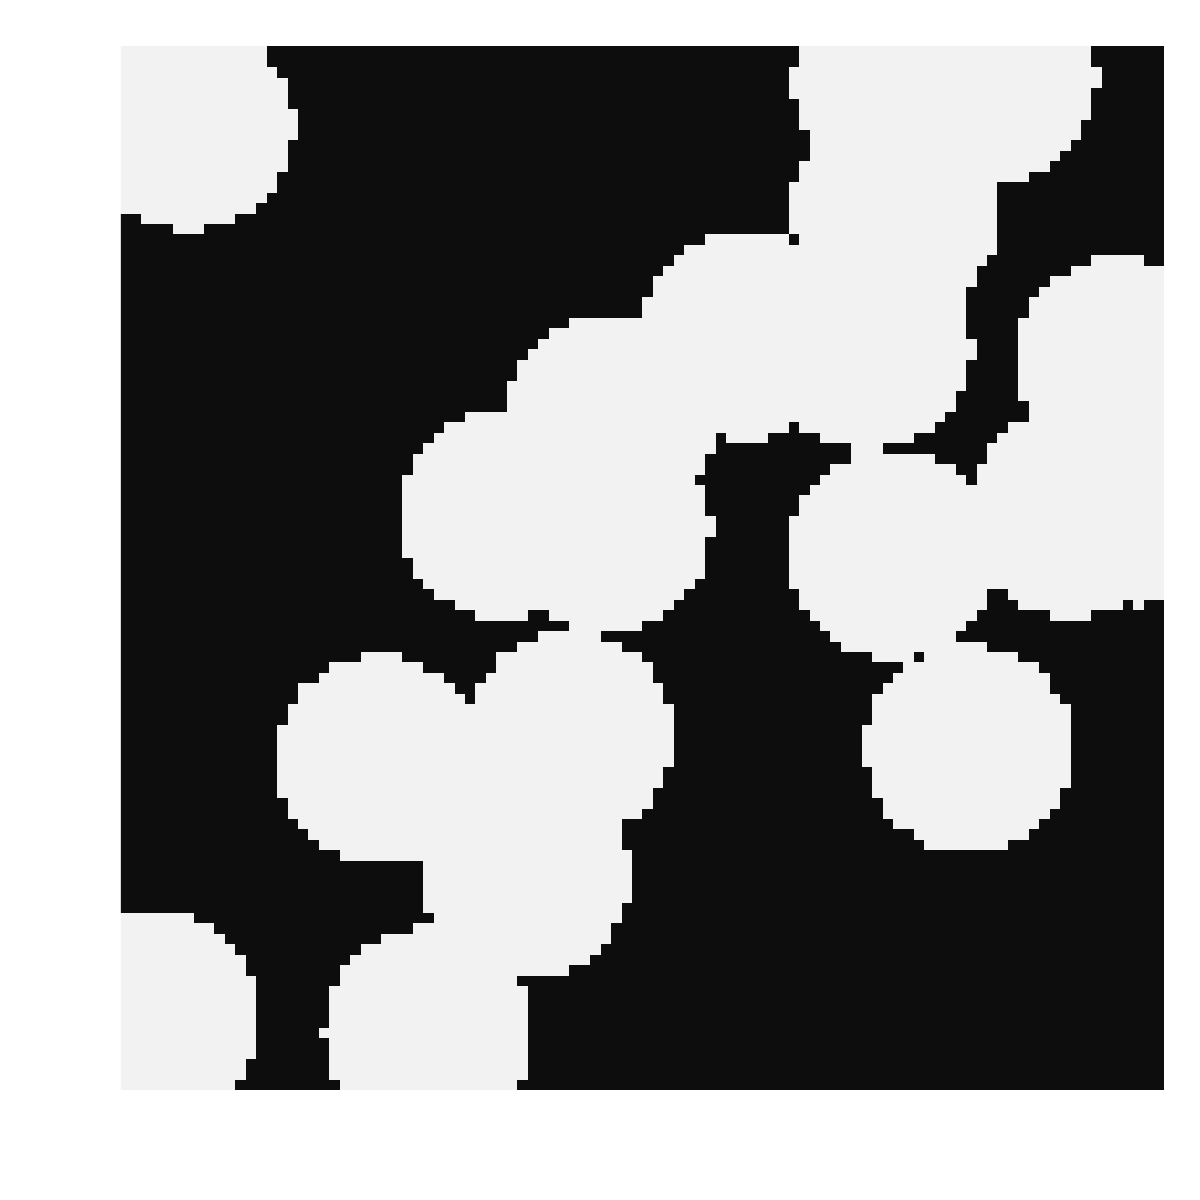
\includegraphics[width=0.32\linewidth]{images/original.png}
  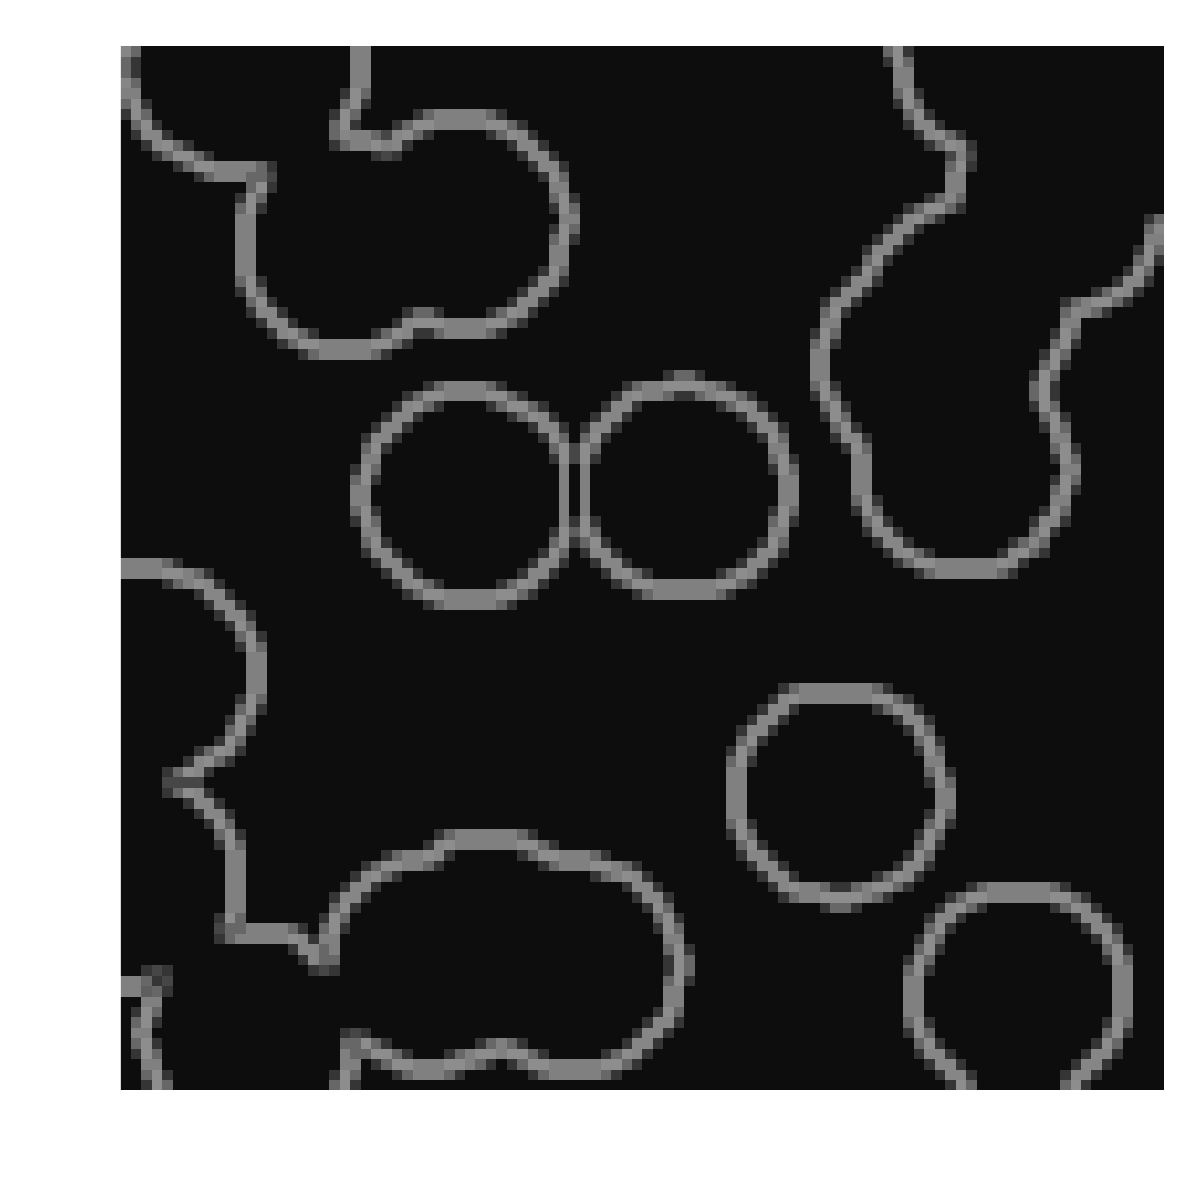
\includegraphics[width=0.32\linewidth]{images/sobel.png}
  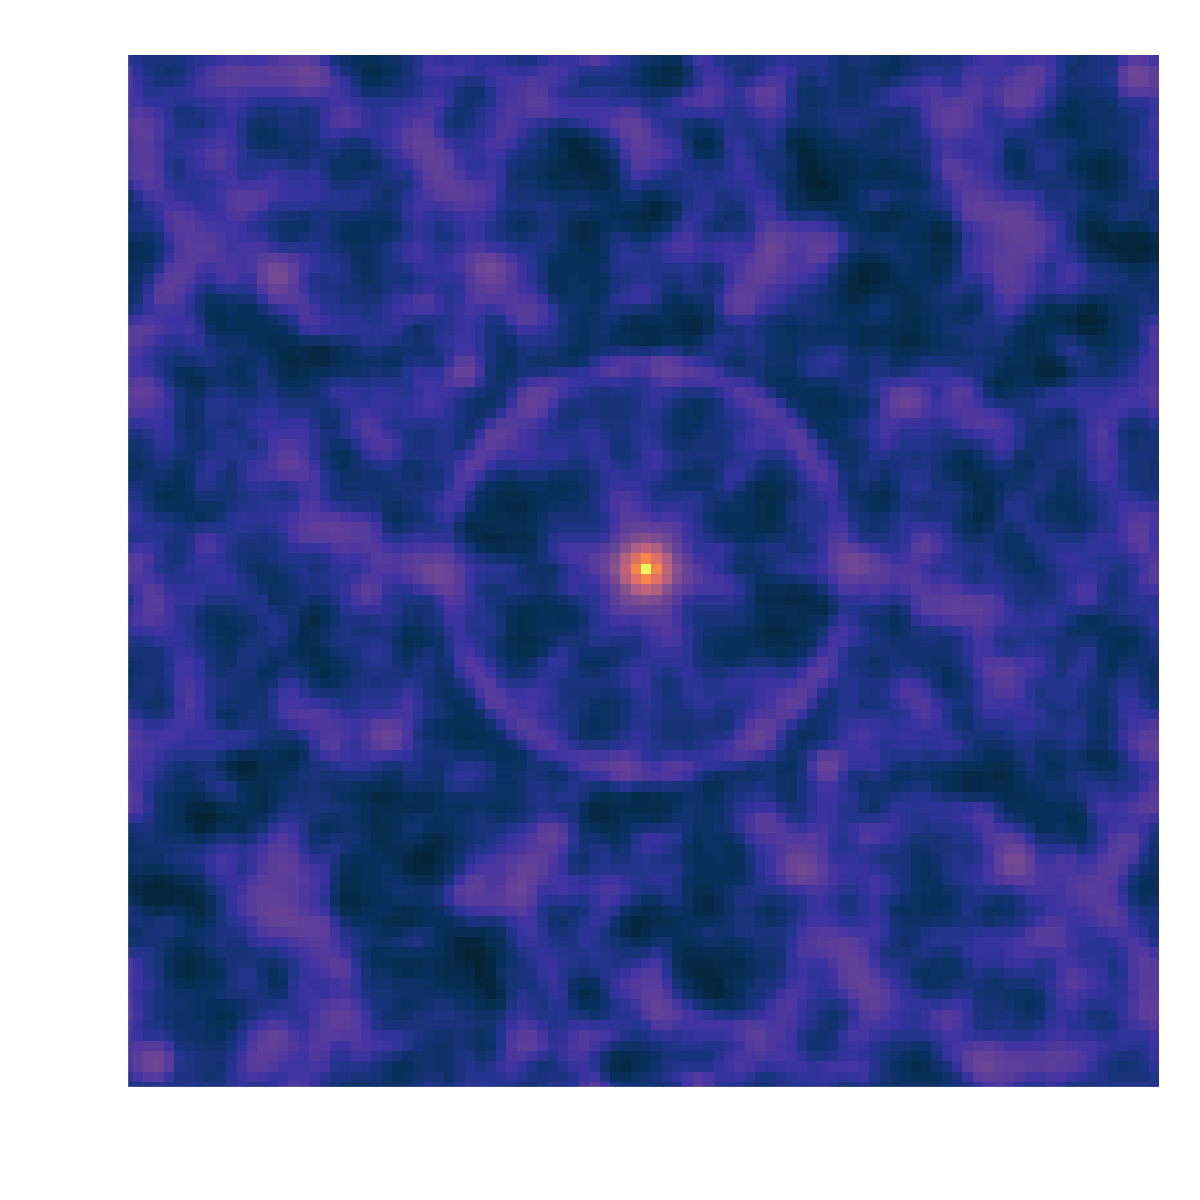
\includegraphics[width=0.32\linewidth]{images/Fss_map_sobel.png}
  \caption{Steps of $F_{ss}$ algorithm using Sobel kernel}
  \label{fig:stages}
\end{figure}
\begin{figure}[ht]
  \centering
  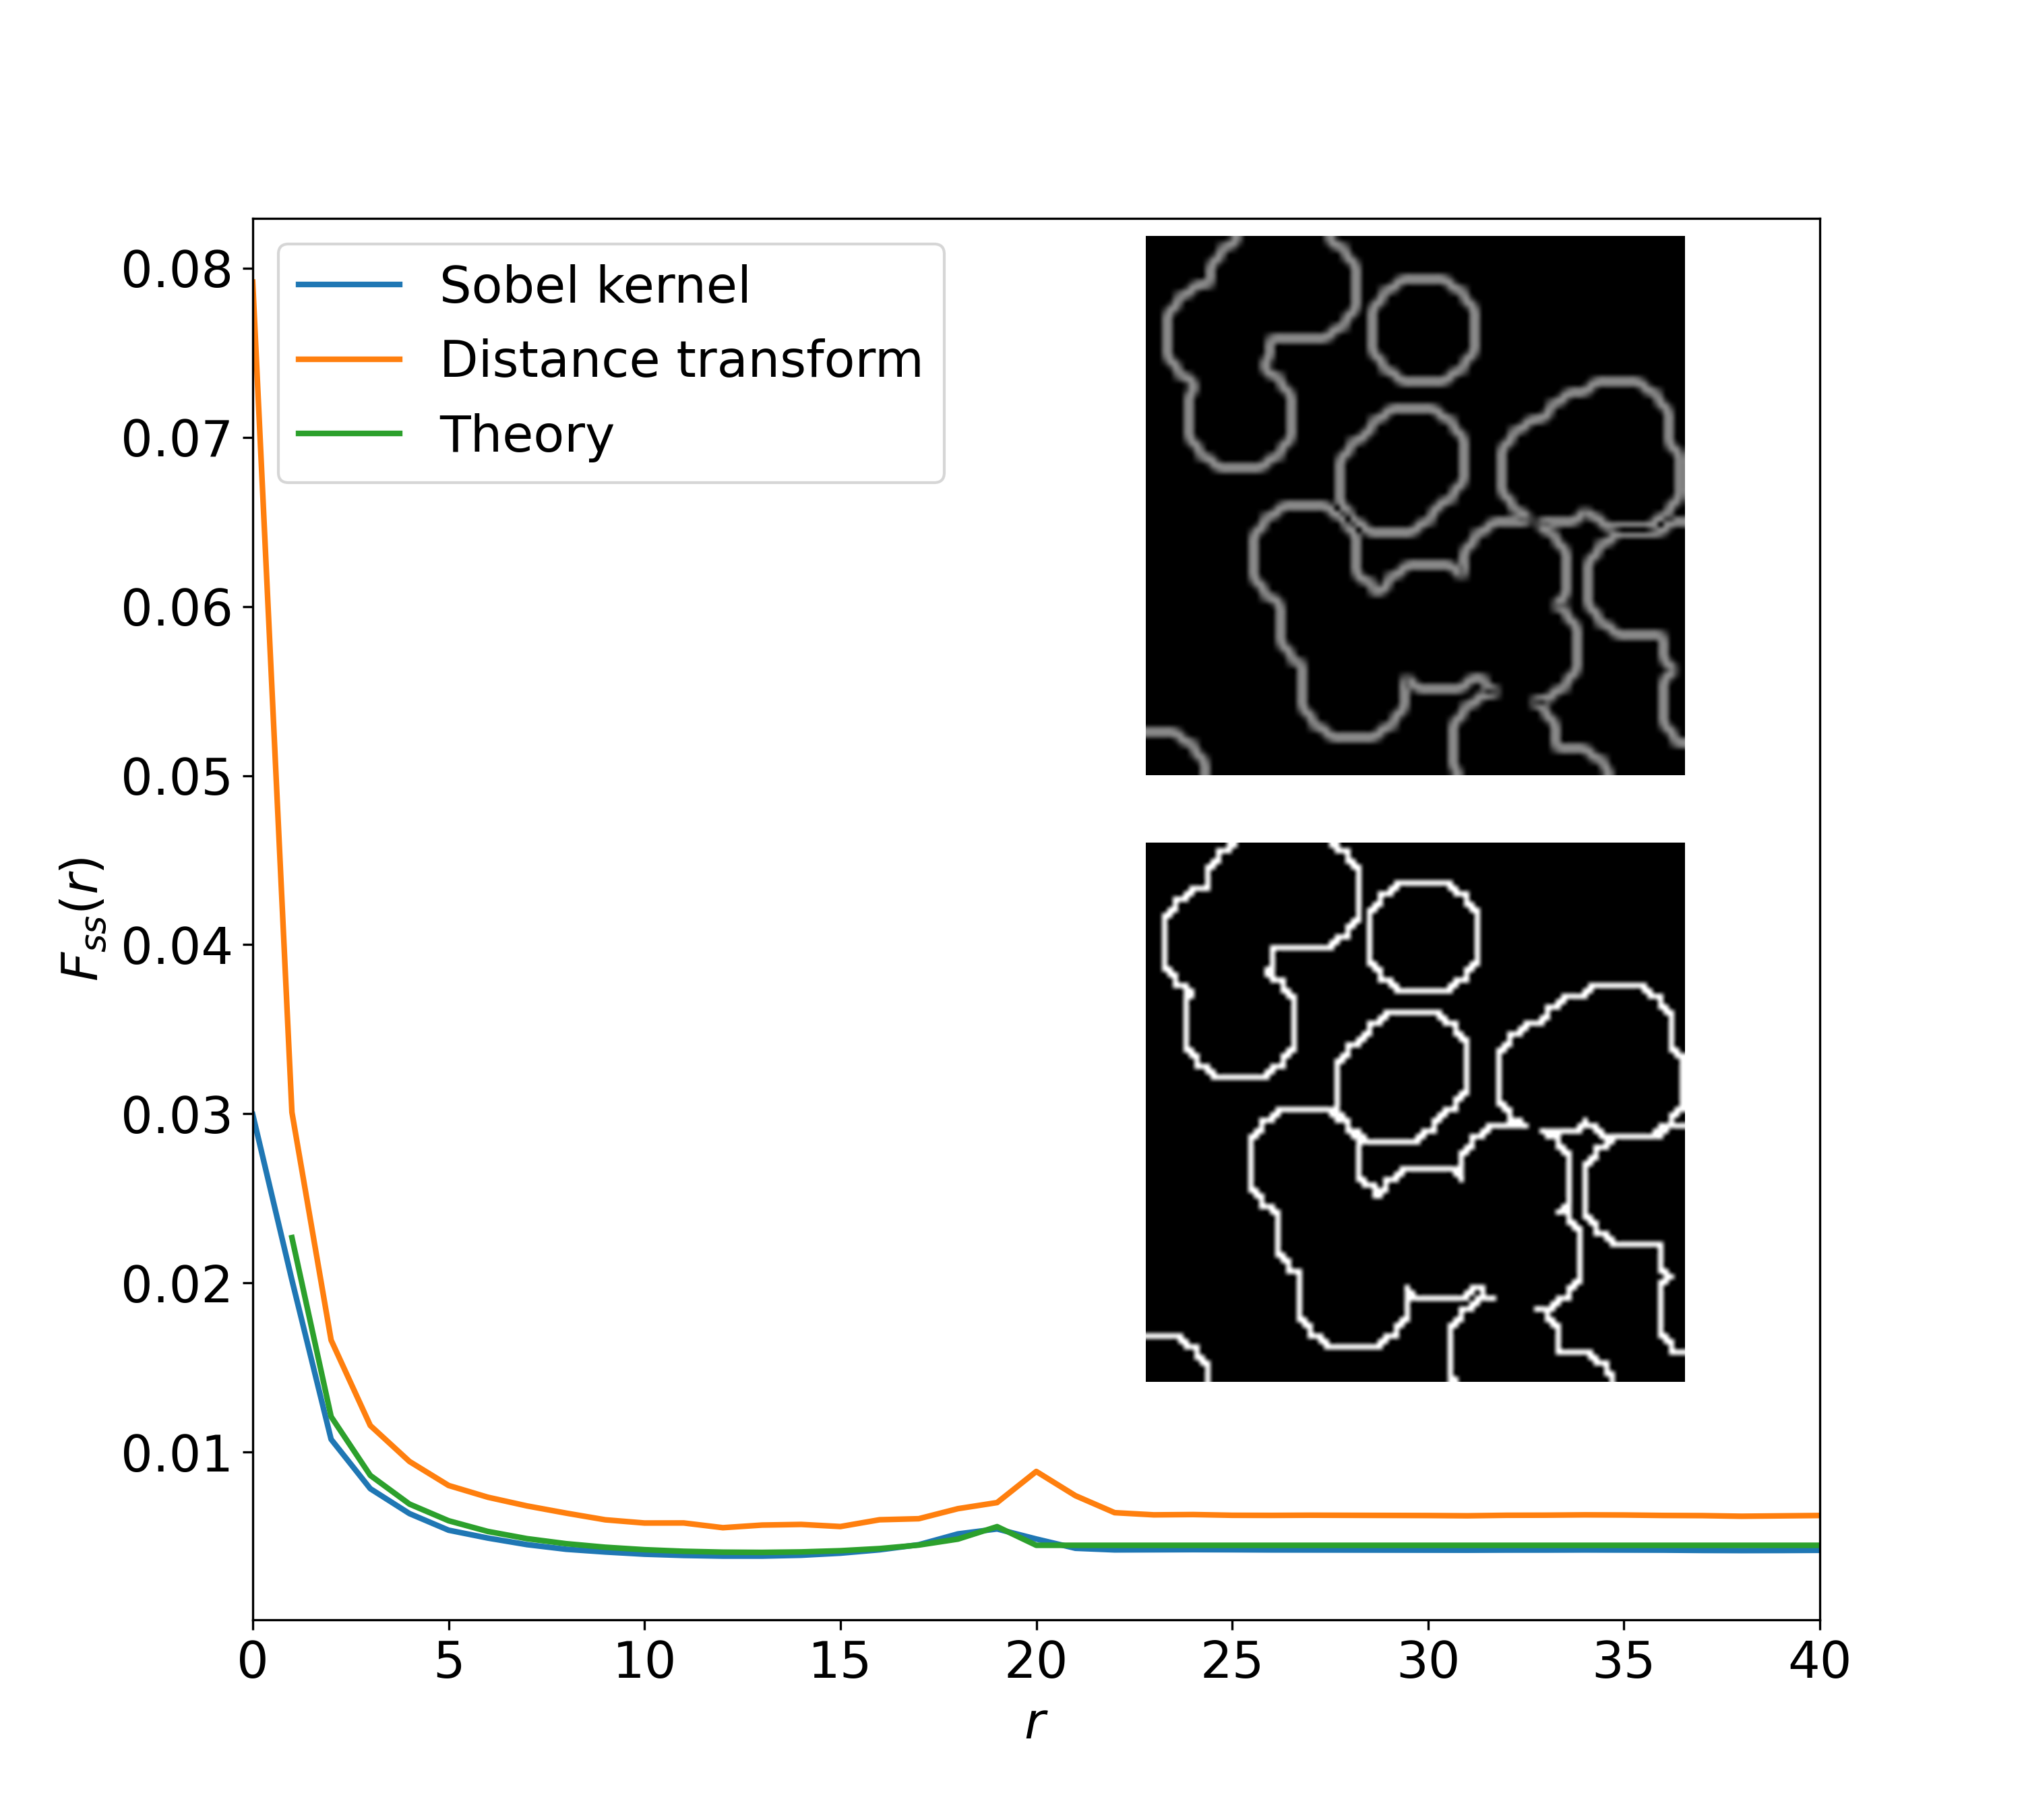
\includegraphics[width=0.99\linewidth]{images/dm_sobel.png}
  \caption{Surface-surface correlation function calculated with different
    interface extraction methods (Sobel on the top, distance map on the
    bottom).}
  \label{fig:interface-extraction}
\end{figure}
\begin{figure}[ht]
  \centering
  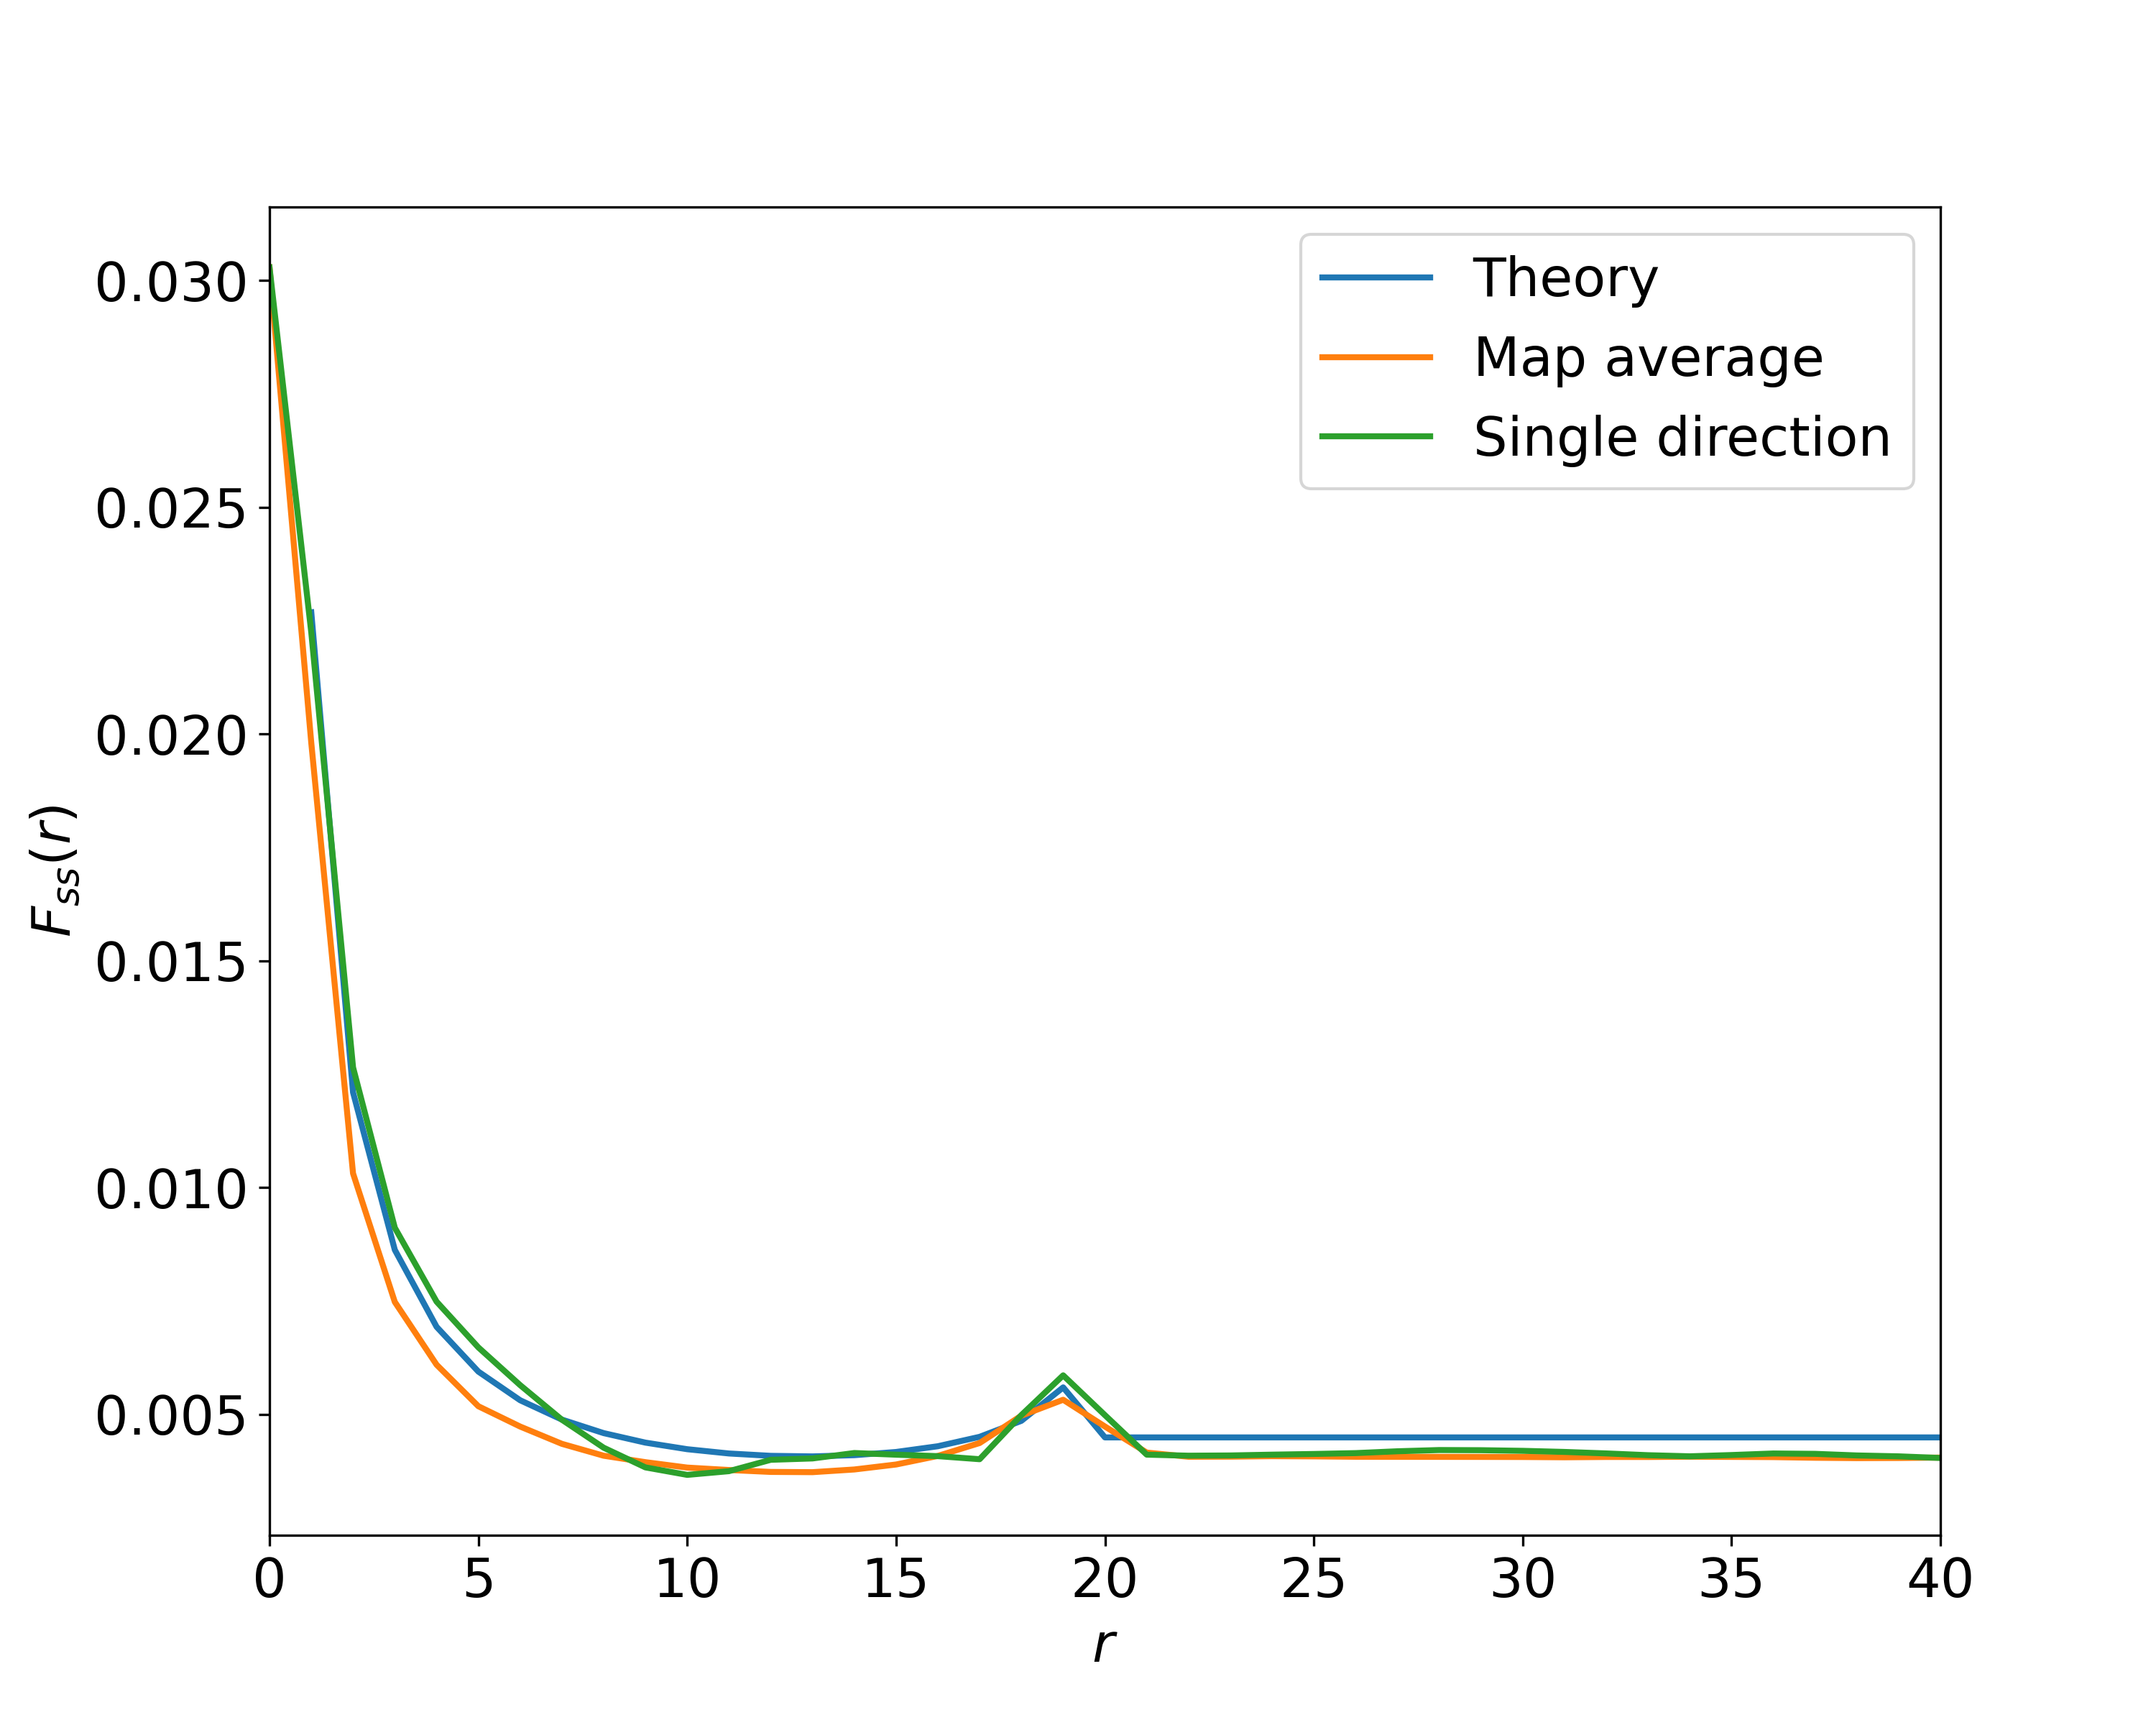
\includegraphics[width=0.99\linewidth]{images/direction_and_map.png}
  \caption{Single direction $F_{ss}$ vs map average comparison}
  \label{fig:direction-vs-map}
\end{figure}

\textit{Distance map}.
One solution to extract ane interface from an image is to use the distance map
(also called the distance transform). Distance transform is a mapping from a
binary image to a scalar field using one of the following functions:
\begin{align}
  D_{o}(\mathbf{x}) &= \left\{
  \begin{array}{ll}
    0 & \quad \mathbf{x} \in V_{void} \\
    \min \rho(\mathbf{x}, \mathbf{y}) \ \forall \mathbf{y} \in V_{void} & \quad \text{otherwise}
  \end{array}
  \right. \label{eq:dist-outer} \\
  D_{i}(\mathbf{x}) &= \left\{
  \begin{array}{ll}
    0 & \quad \mathbf{x} \not\in V_{void} \\
    \min \rho(\mathbf{x}, \mathbf{y}) \ \forall \mathbf{y} \not\in V_{void} & \quad \text{otherwise}
  \end{array}
  \right. \label{eq:dist-inner}
\end{align}
where $V_{void}$ is a set containing elements belonging to the void phase and
$\rho(\mathbf{x}, \mathbf{y})$ is the Euclidean distance between points
$\mathbf{x}$ and $\mathbf{y}$. Now $M(\mathbf{x})$ in \cref{eq:interface} may be
written as follows:
\begin{equation*}
  M(\mathbf{x}) = \left\{
  \begin{array}{ll}
    1 & 0 < \quad D(\mathbf{x}) \le \sqrt{d} \\
    0 & \quad \text{otherwise}
  \end{array}
  \right.
\end{equation*}
where $d$ is dimensionality of the image ($d = 2$ for 2D image, $d = 3$ for 3D
image) and $D(\mathbf{x})$ is either \cref{eq:dist-outer} or
\cref{eq:dist-outer}. When $D = D_i$ we call the resulting interface
``inner interface'' and when $D = D_o$ we call it ``outer interface''.

\textit{Image filtering}.
This method creates grayscale image of the interface. We use Sobel operator $S$
to detect edges of the image $A'$, so $M = S$ in algorithms in
\cref{sec:general}. We calculate $\|S(A')\|$ element-wise ($\|\cdot\|$ denotes
the usual norm on Euclidean space). This norm can be interpreted as the
probability that a point in $A$ belongs to the interface. In a digitized image
$\|S(A')\|$ can be represented as an array of floating point numbers having the
same shape as an original image $A$.

\subsection{Computing correlation}
We will describe method of computing cross correlation function between two
images $f$ and $g$: $\star (f, g)$. In the case of auto correlation function we
assume $f = g$. Algorithm is straightforward when boundary conditions are
periodic. For non-periodic boundary conditions we will need a minor change.

\textit{Periodic boundary condition}
\begin{algorithmic}[1]
  \Procedure{$\star$}{$f, g$}
  \State $\hat{f} = F(f)$
  \State $\hat{g} = F(g)$
  \Comment Compute FFT of the input.
  \State $\hat{cc} \gets \hat{f} \cdot \overline{\hat{g}}$
  \Comment Multiply element-wise.
  \State $cc \gets F^{-1}(\hat{cc})$
  \Comment Compute IFFT of $\hat{cc}$.
  \State \textbf{return} $cc$ divided by the number of pixels in the input.
  \EndProcedure
\end{algorithmic}

\textit{Non-periodic boundary condition}
\begin{algorithmic}[1]
  \Procedure{$\star$}{$f, g$}
  \State Pad $f$ and $g$ with zeros in each dimension to the size $2n-1$ where
  $n$ is the size of the image in that dimension.
  \State $\hat{f} = F(f)$
  \State $\hat{g} = F(g)$
  \Comment Compute FFT of the input.
  \State $\hat{cc} \gets \hat{f} \cdot \overline{\hat{g}}$
  \Comment Multiply element-wise.
  \State $cc \gets F^{-1}(\hat{cc})$
  \Comment Compute IFFT of $\hat{cc}$.
  \State circle shift $cc$ by $n - 1$ in each direction, so index range becomes
  from $-(n - 1)$ to $n - 1$.
  \State $cc_{ij} \gets cc_{ij} / q_{ij}$ where $q_{ij} = (n - |i|)(m - |j|)$
  \Comment Divide each element $cc_{ij}$ by the number of pixels whose
  coordinate difference is equal to $(i, j)$.
  \State \textbf{return} $cc$.
  \EndProcedure
\end{algorithmic}

Consecutive stages of our method are shown in \cref{fig:stages}. It is also a
part of \code{CorrelationFunctions.jl} package \cite{CFsjlpaper} for Julia
programming language that allows to compute all classical CFs described in
Torquato’s book \cite{Torquato_book} from digital images.

\section{Application to synthetic and real binary 2D/3D images}
\label{sec:results}
\subsection{Comparisons against analytical solutions}
\label{sec:comparison}
To evaluate the accuracy of surface CFs computations the most straightforward
way is to compare them against analytical solutions. We use well-known
analytical soulution for overlapping disks and balls with fixed radius $R$ and
centers generated by Poisson point process with parameter $\lambda$. Starting
with an image with resolution of $4096 \times 4096$ pixels, we then downscale it
by 4, 16, and 64 times with the help of bicubic interpolation
\cite{ledesma2018effect}. We show that calculated correlation functions approach
theoretical values when the resolution is high enough.

It is easy to show that assuming $a > 0$:
\begin{align}
  a^2 F_{ss}(a \mathbf{x}, a(\mathbf{x} + \mathbf{r})) &= F_{ss}(\mathbf{x},
  \mathbf{x} + \mathbf{r}) \label{eq:scale-ss} \\
  a F_{sv}(a \mathbf{x}, a(\mathbf{x} + \mathbf{r})) &= F_{sv}(\mathbf{x},
  \mathbf{x} + \mathbf{r}) \label{eq:scale-sv}
\end{align}
Assuming that our images represent homogeneous and isotropic media, we calculate
$F_{ss}(ar)$ and $F_{sv}(ar)$ for each original and rescaled image and multiply
it by coefficient $a^2 = (L_{scaled}/L_{orig})^2$ and $a = L_{scaled}/L_{orig}$
respectively, where $L_{scaled}$ is the side of the rescaled image and
$L_{orig}$ is the side of the original image. The resulting scaled surface CFs
are shown in \cref{fig:scaling}.

\begin{figure*}[ht]
  \centering
  \subfigure[Surface-surface]{
    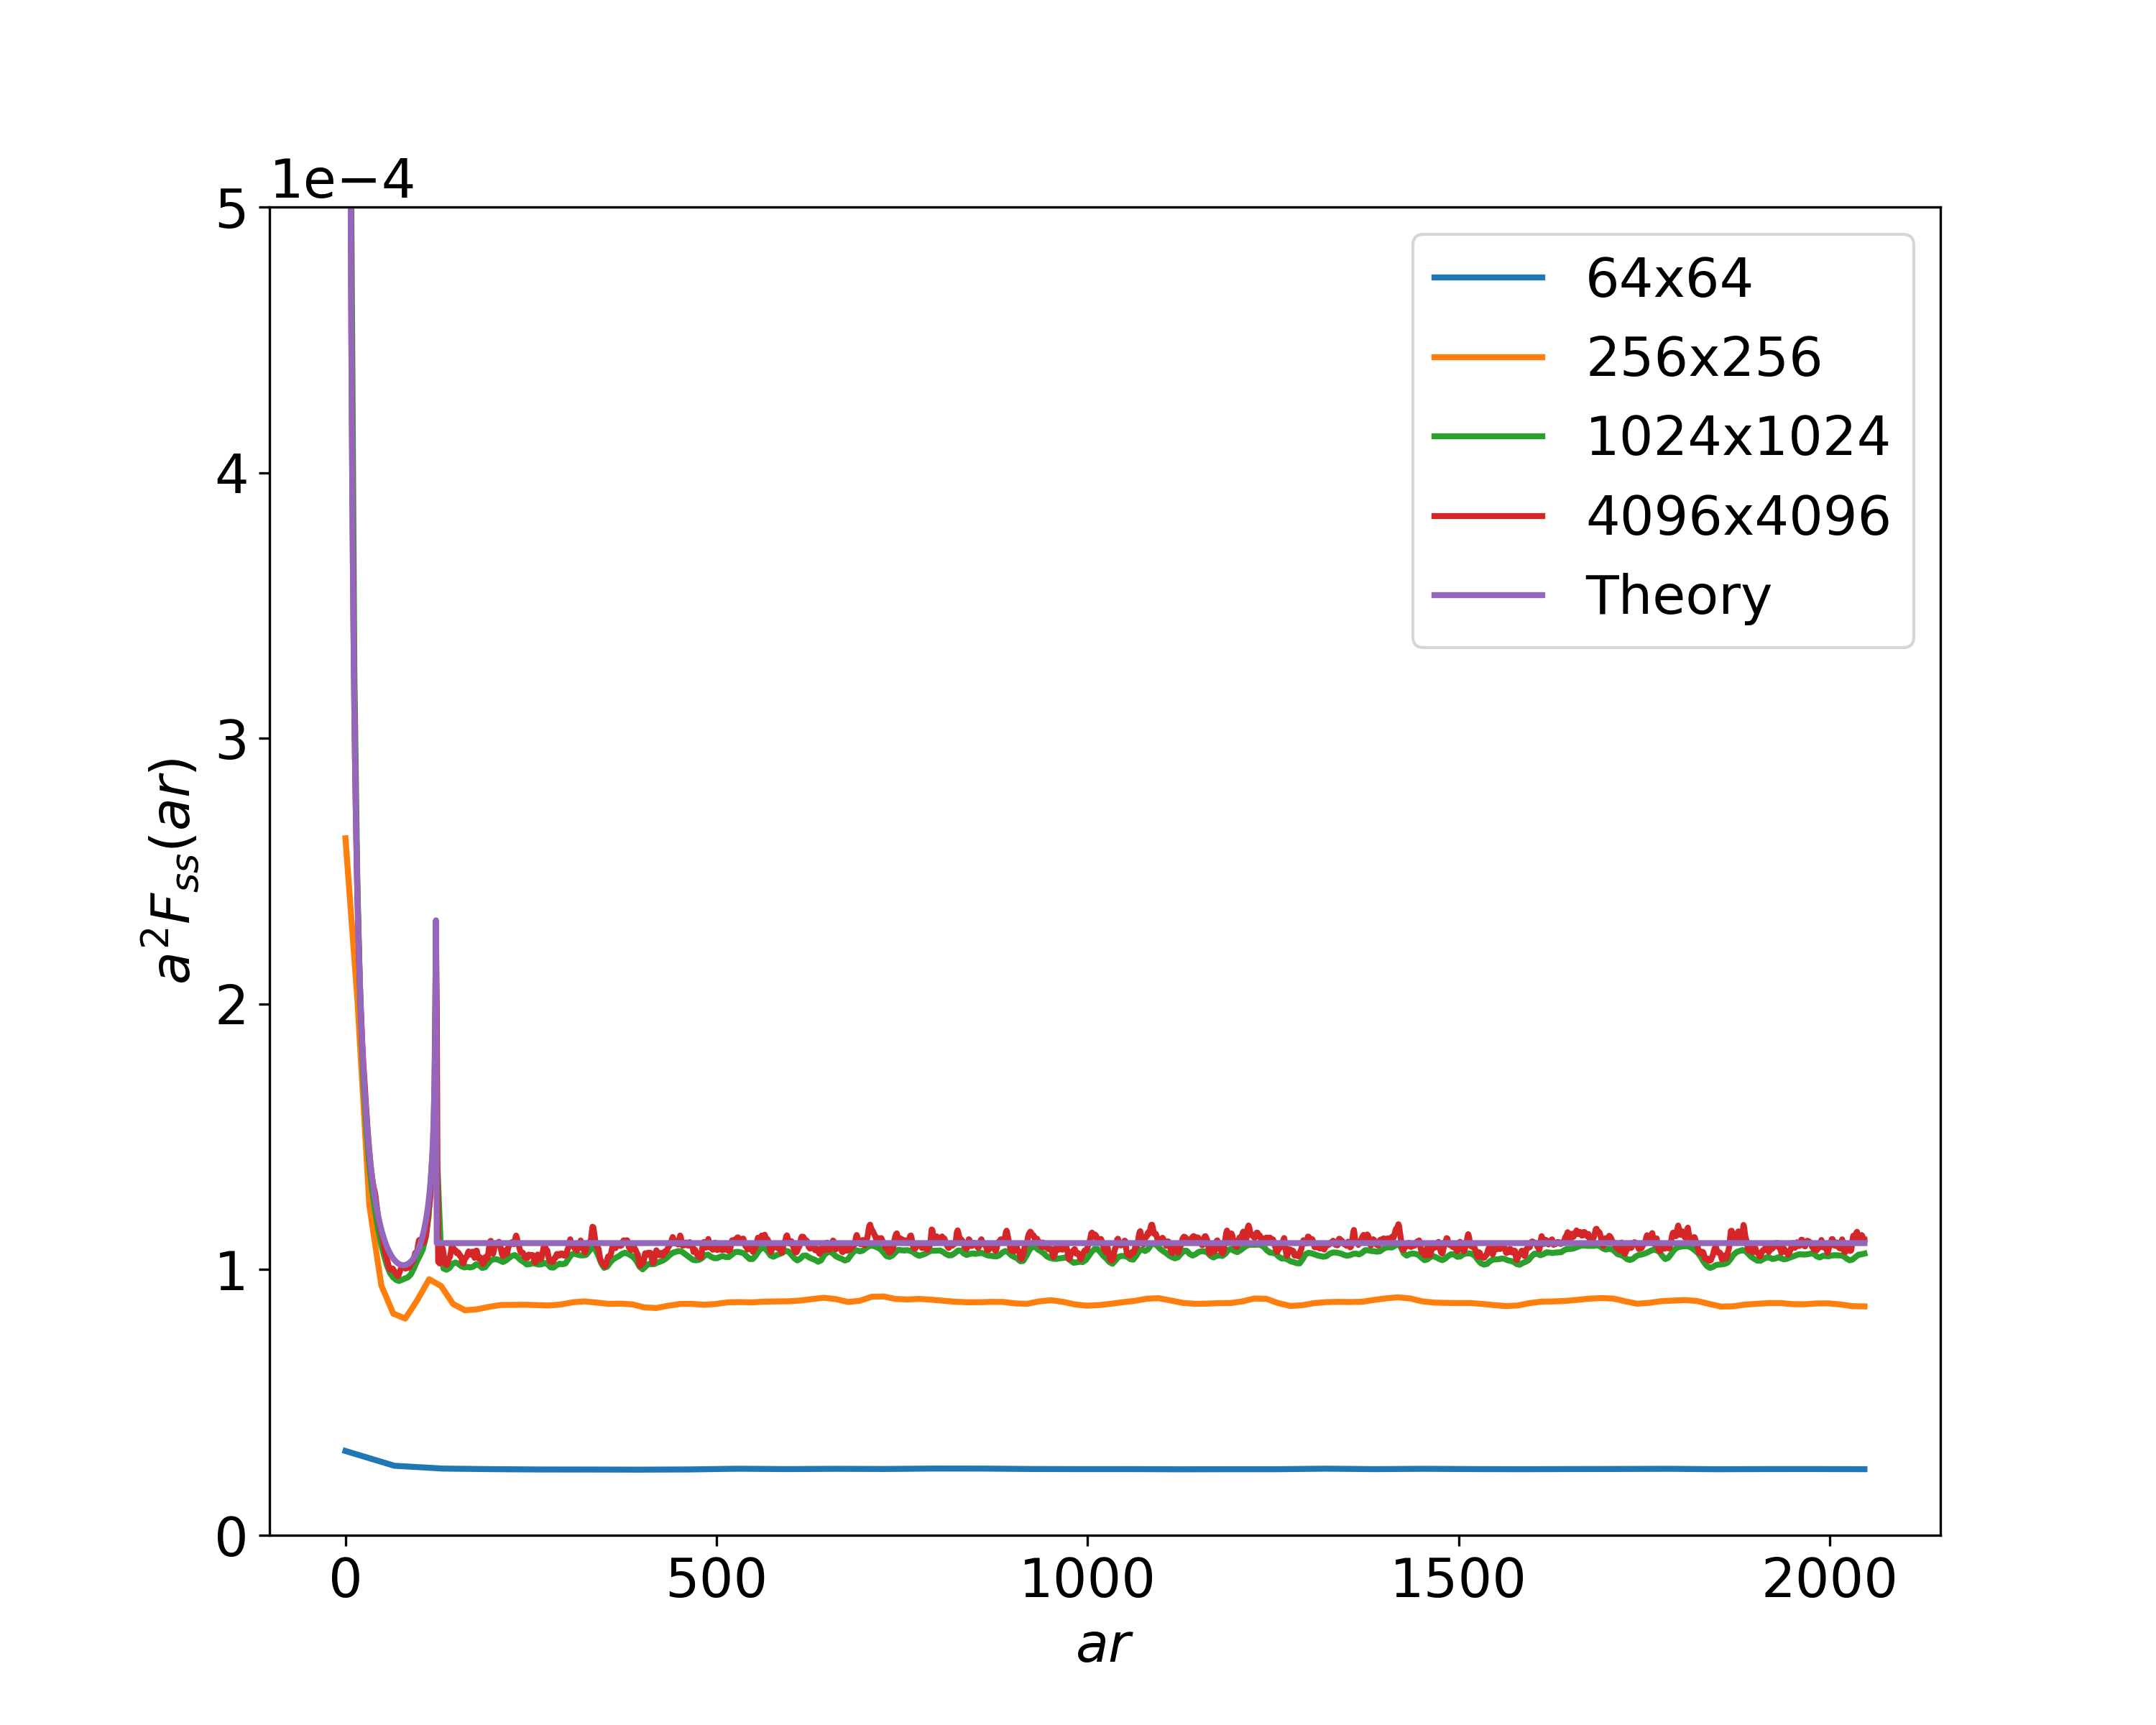
\includegraphics[width=0.475\linewidth]{images/plot-ss-balls.png}
    \label{fig:fss-scaling}}
  \hfill
  \subfigure[Surface-void]{
    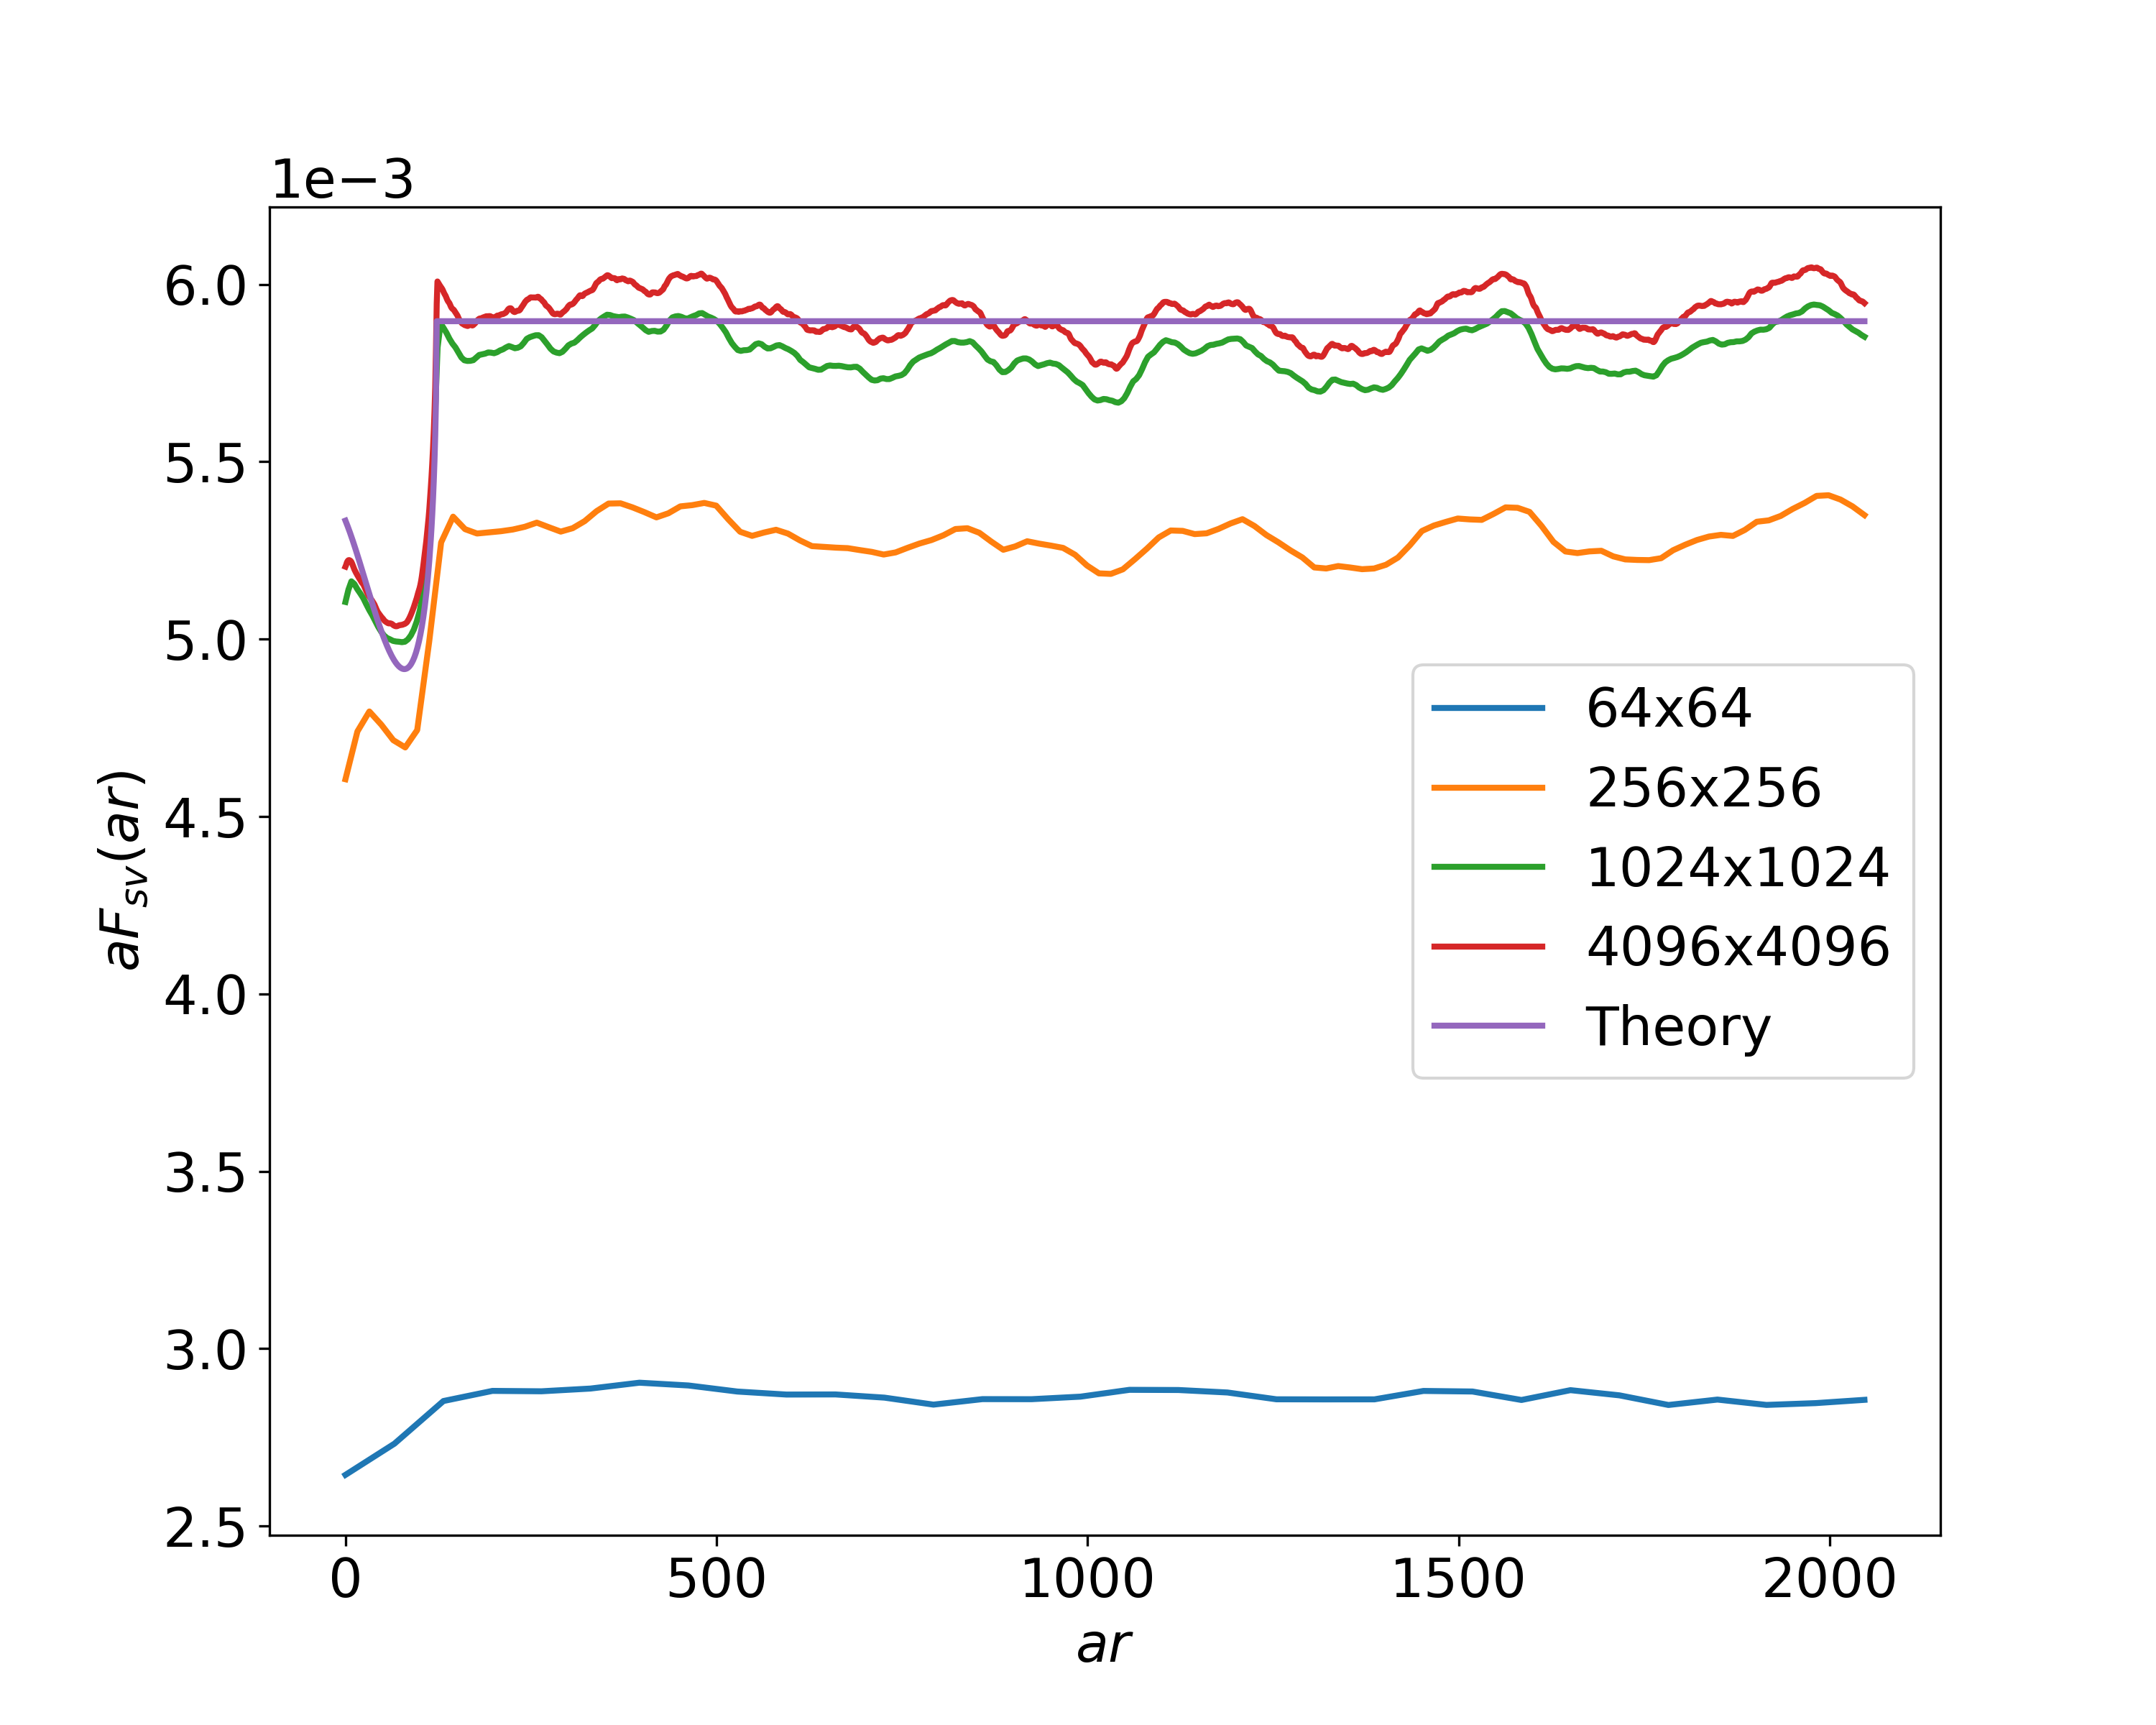
\includegraphics[width=0.475\linewidth]{images/plot-sv-balls.png}
    \label{fig:fsv-scaling}}
    \caption[]{The comparison of analytical and computed surface correlation
      functions for the Poisson disks for the original $4096 \times 4096$ pixels
      image. Computed CFs were obtained for different image resolutions as shown
      in the legend.}
    \label{fig:scaling}
\end{figure*}

We can observe two effects when downscaling the original image. The
first effect is that $F_{ss}(ar)$ and $F_{sv}(ar)$ for downscaled images lack in
detail (i.e. they are less ``noisy''). This can be easily explained by that the
interface between phases that becomes ``simpler'' when resolution decreases. The
second and much more important effect is that both correlation functions become
largely underestimated with the decline in resolution. This latter effect is in
general connected to the fact that the interface in digital images has
non-negligible thickness -- i.~e. the difference between real ``continuous''
interface versus ``digital'' interface (\cref{fig:scheme}). It is logical to
assume that with increasing spatial resolution the influence of this thickness
will diminish. This is exactly what we observe on \cref{fig:scaling} where
increasing disk discretization leads to convergence with analytical solution;
the accuracy of the computed CFs is almost perfect for discretization of about
4096 pixels for each disk. A natural question arises: ``Is there a criterion of
image quality (resolution) that allows to predict the quality of surface CFs
evaluation from digital images?''. Turns out there is a possibility to establish
such empirical criterion based on spectral analysis of input images and
\cref{sec:crit} provides necessary details.

Now consider a situation when an image is obtained by taking samples of a function
$f: \mathbb{R}^n \rightarrow \left\{0, 1\right\}$. The samples are taken from a
regular grid which covers the range $[0, 1]^n$  with interval $\Delta$ between
samples. The resulting image has then $1/\Delta + 1$ pixels in each
dimension. An example of $f$ is a thresholded value noise function, and an
example of image generated by sampling this function is on
\cref{fig:noise}. Correlation functions calculated for the noise at different
resolutions are on \cref{fig:scaling-noise}. If we calculate surface-surface and
surface-void correlation functions for these images and scale them as described
above, we will converge to some ``true'' correlation functions for continuous
function $f$.
\begin{figure}[ht]
  \centering
  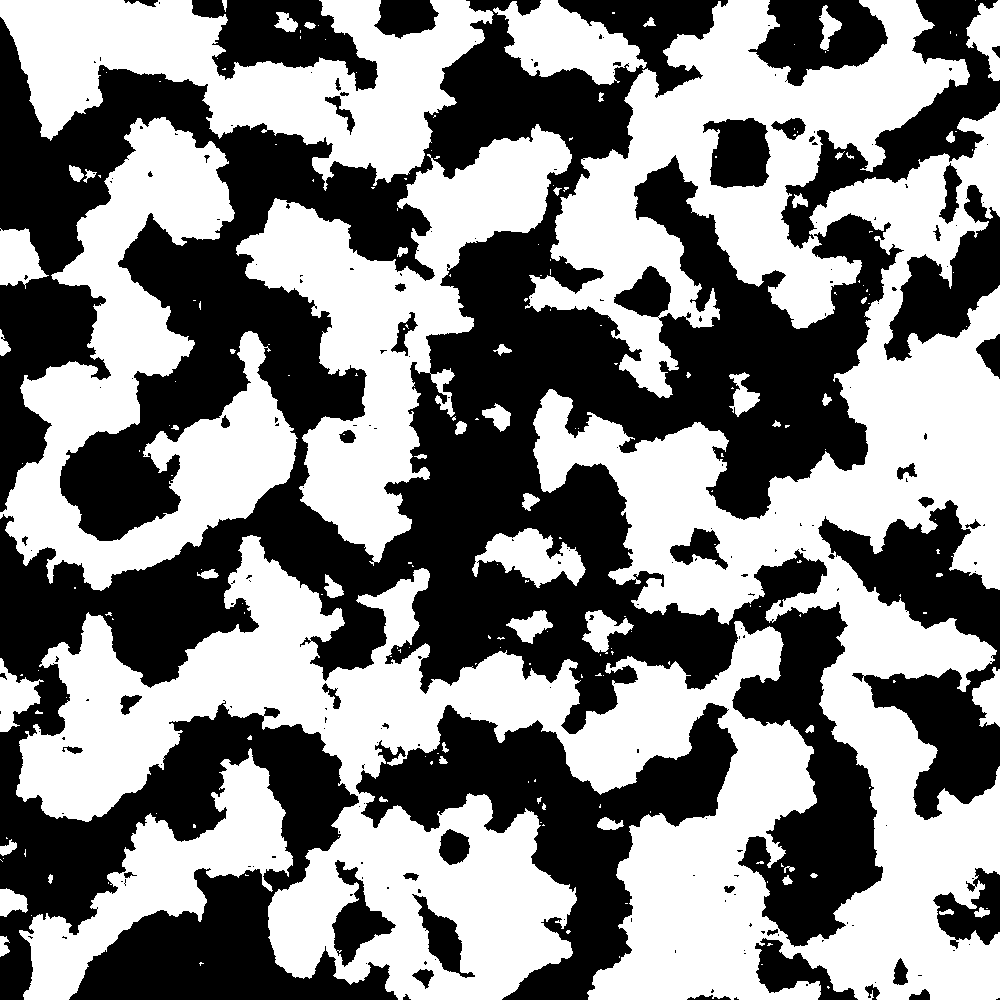
\includegraphics[width=0.9\linewidth]{images/noise.png}
  \caption[]{Example of thresholded value noise used for study of sampling
    effects.}
  \label{fig:noise}
\end{figure}

\begin{figure*}[ht]
  \centering
  \subfigure[Surface-surface]{
    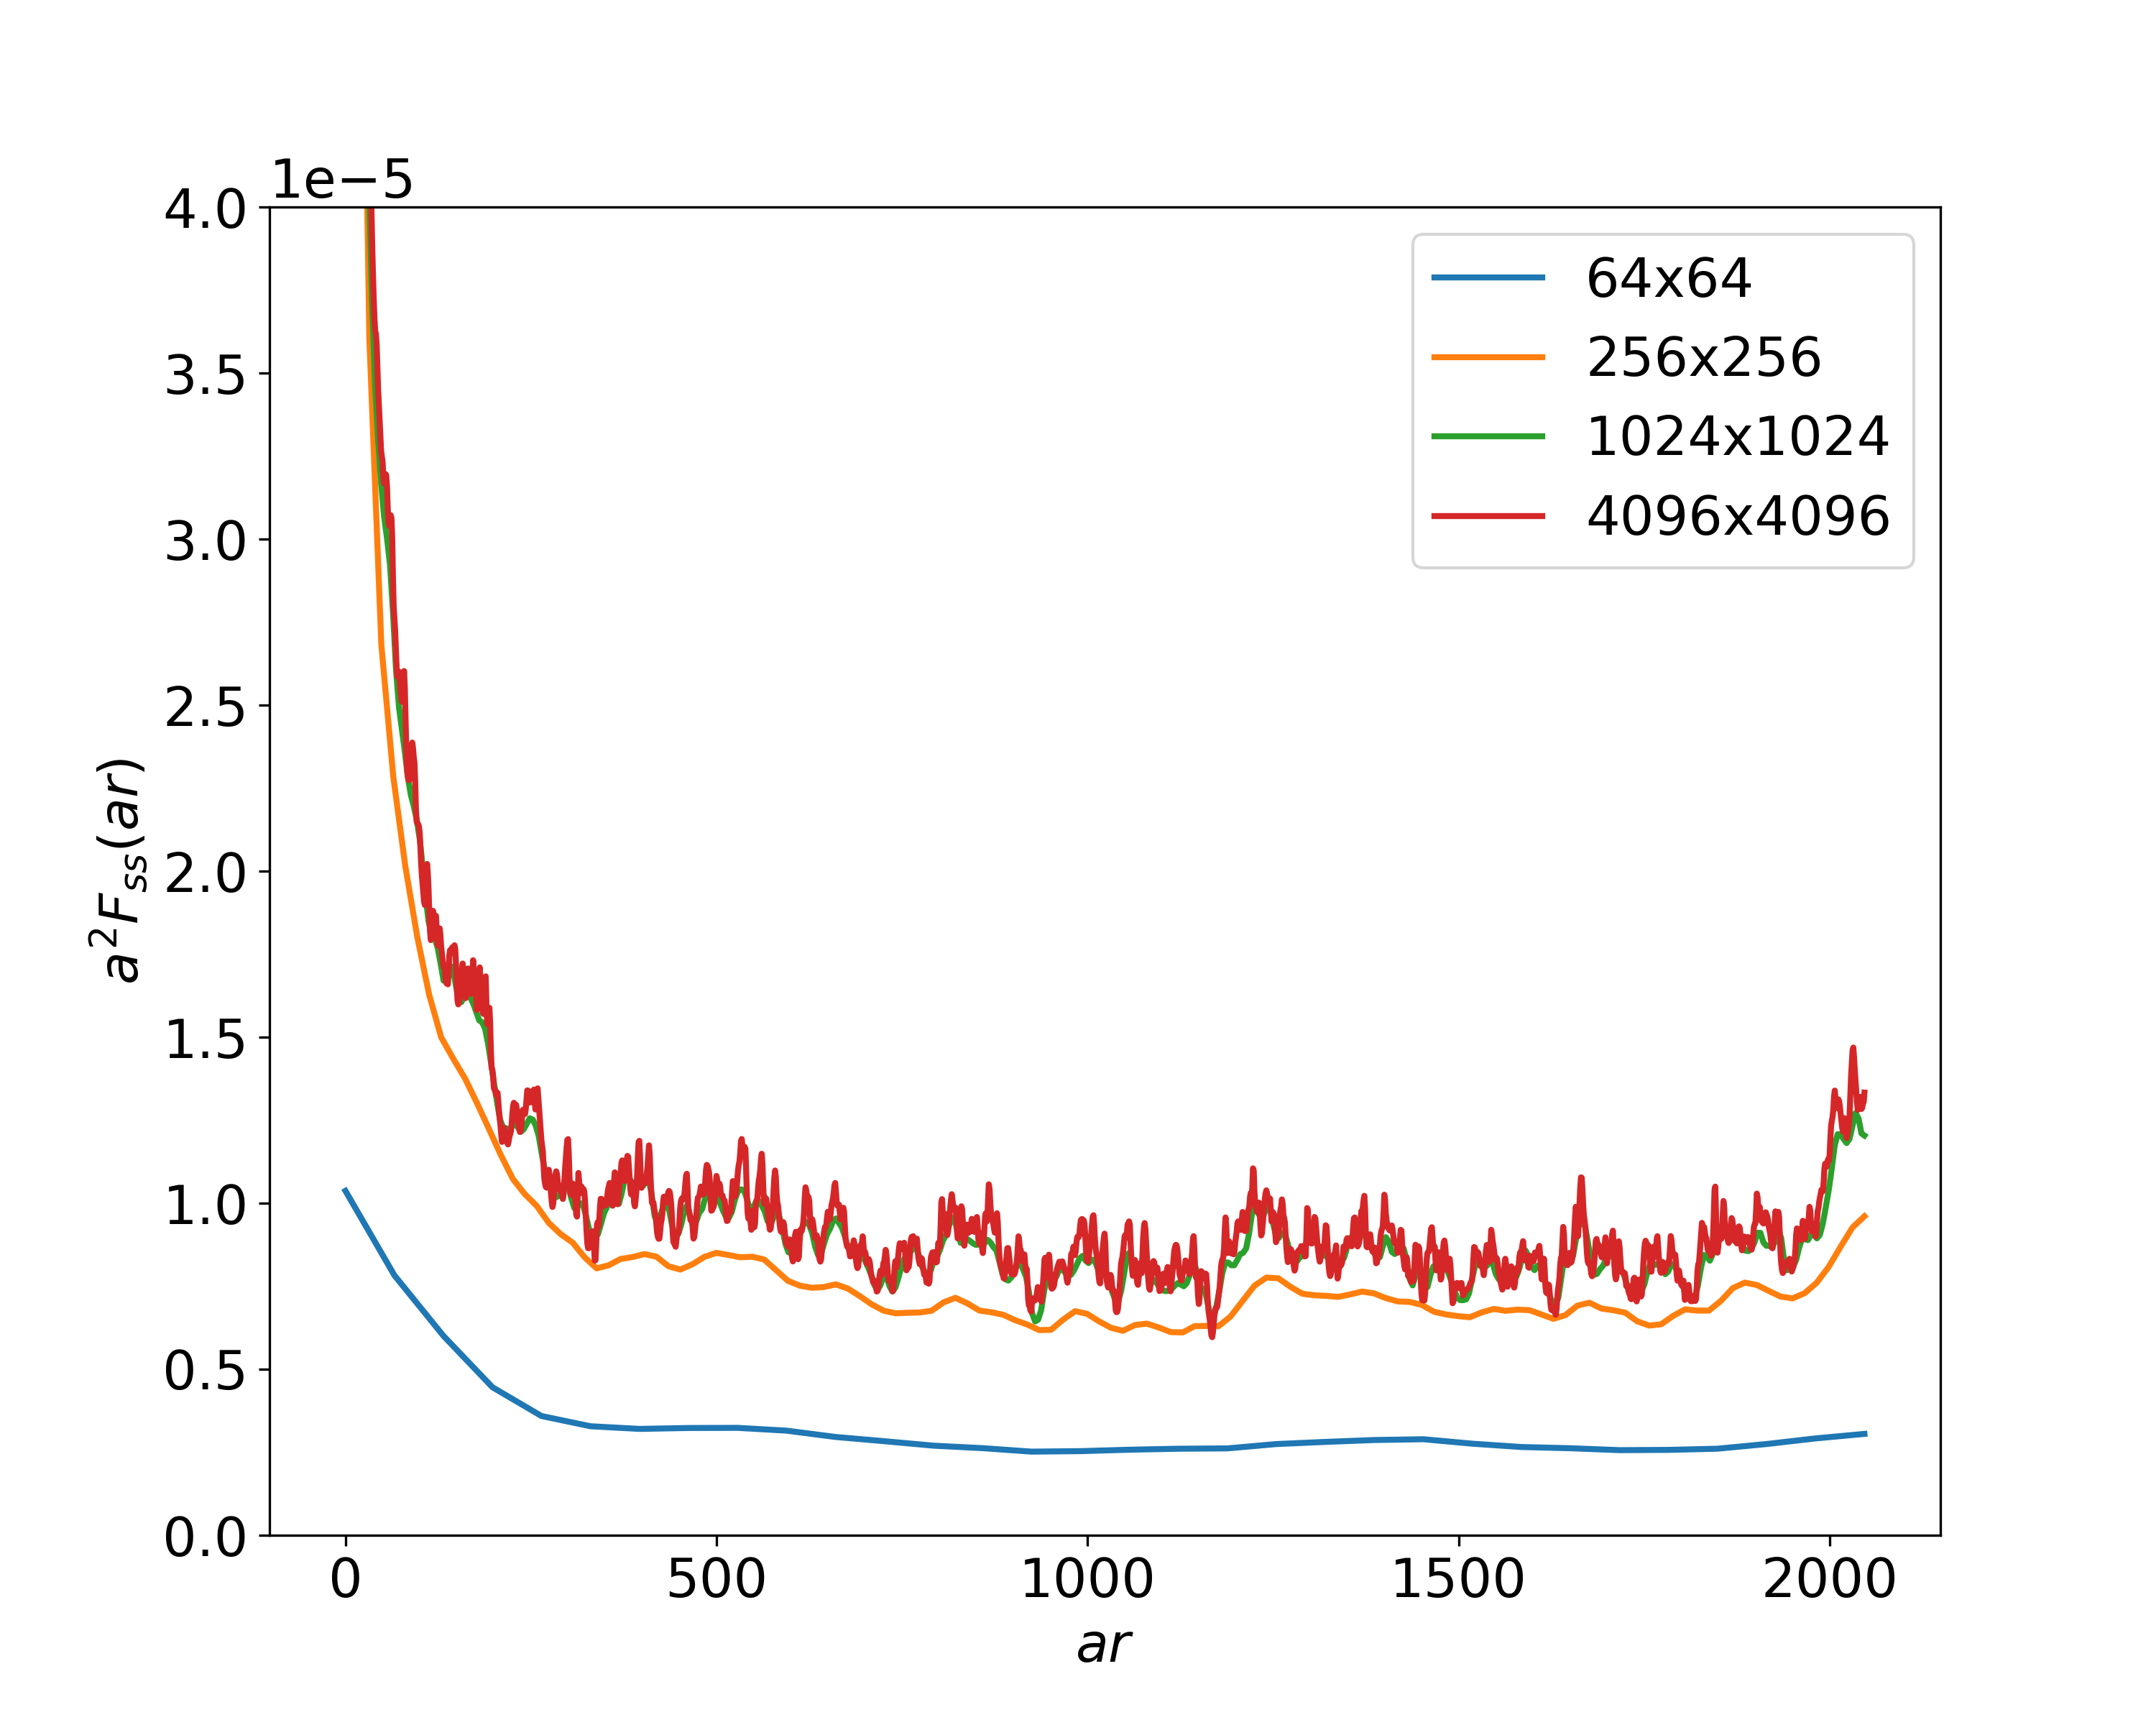
\includegraphics[width=0.475\linewidth]{images/plot-ss-noise.png}
    \label{fig:fss-scaling-noise}}
  \hfill
  \subfigure[Surface-void]{
    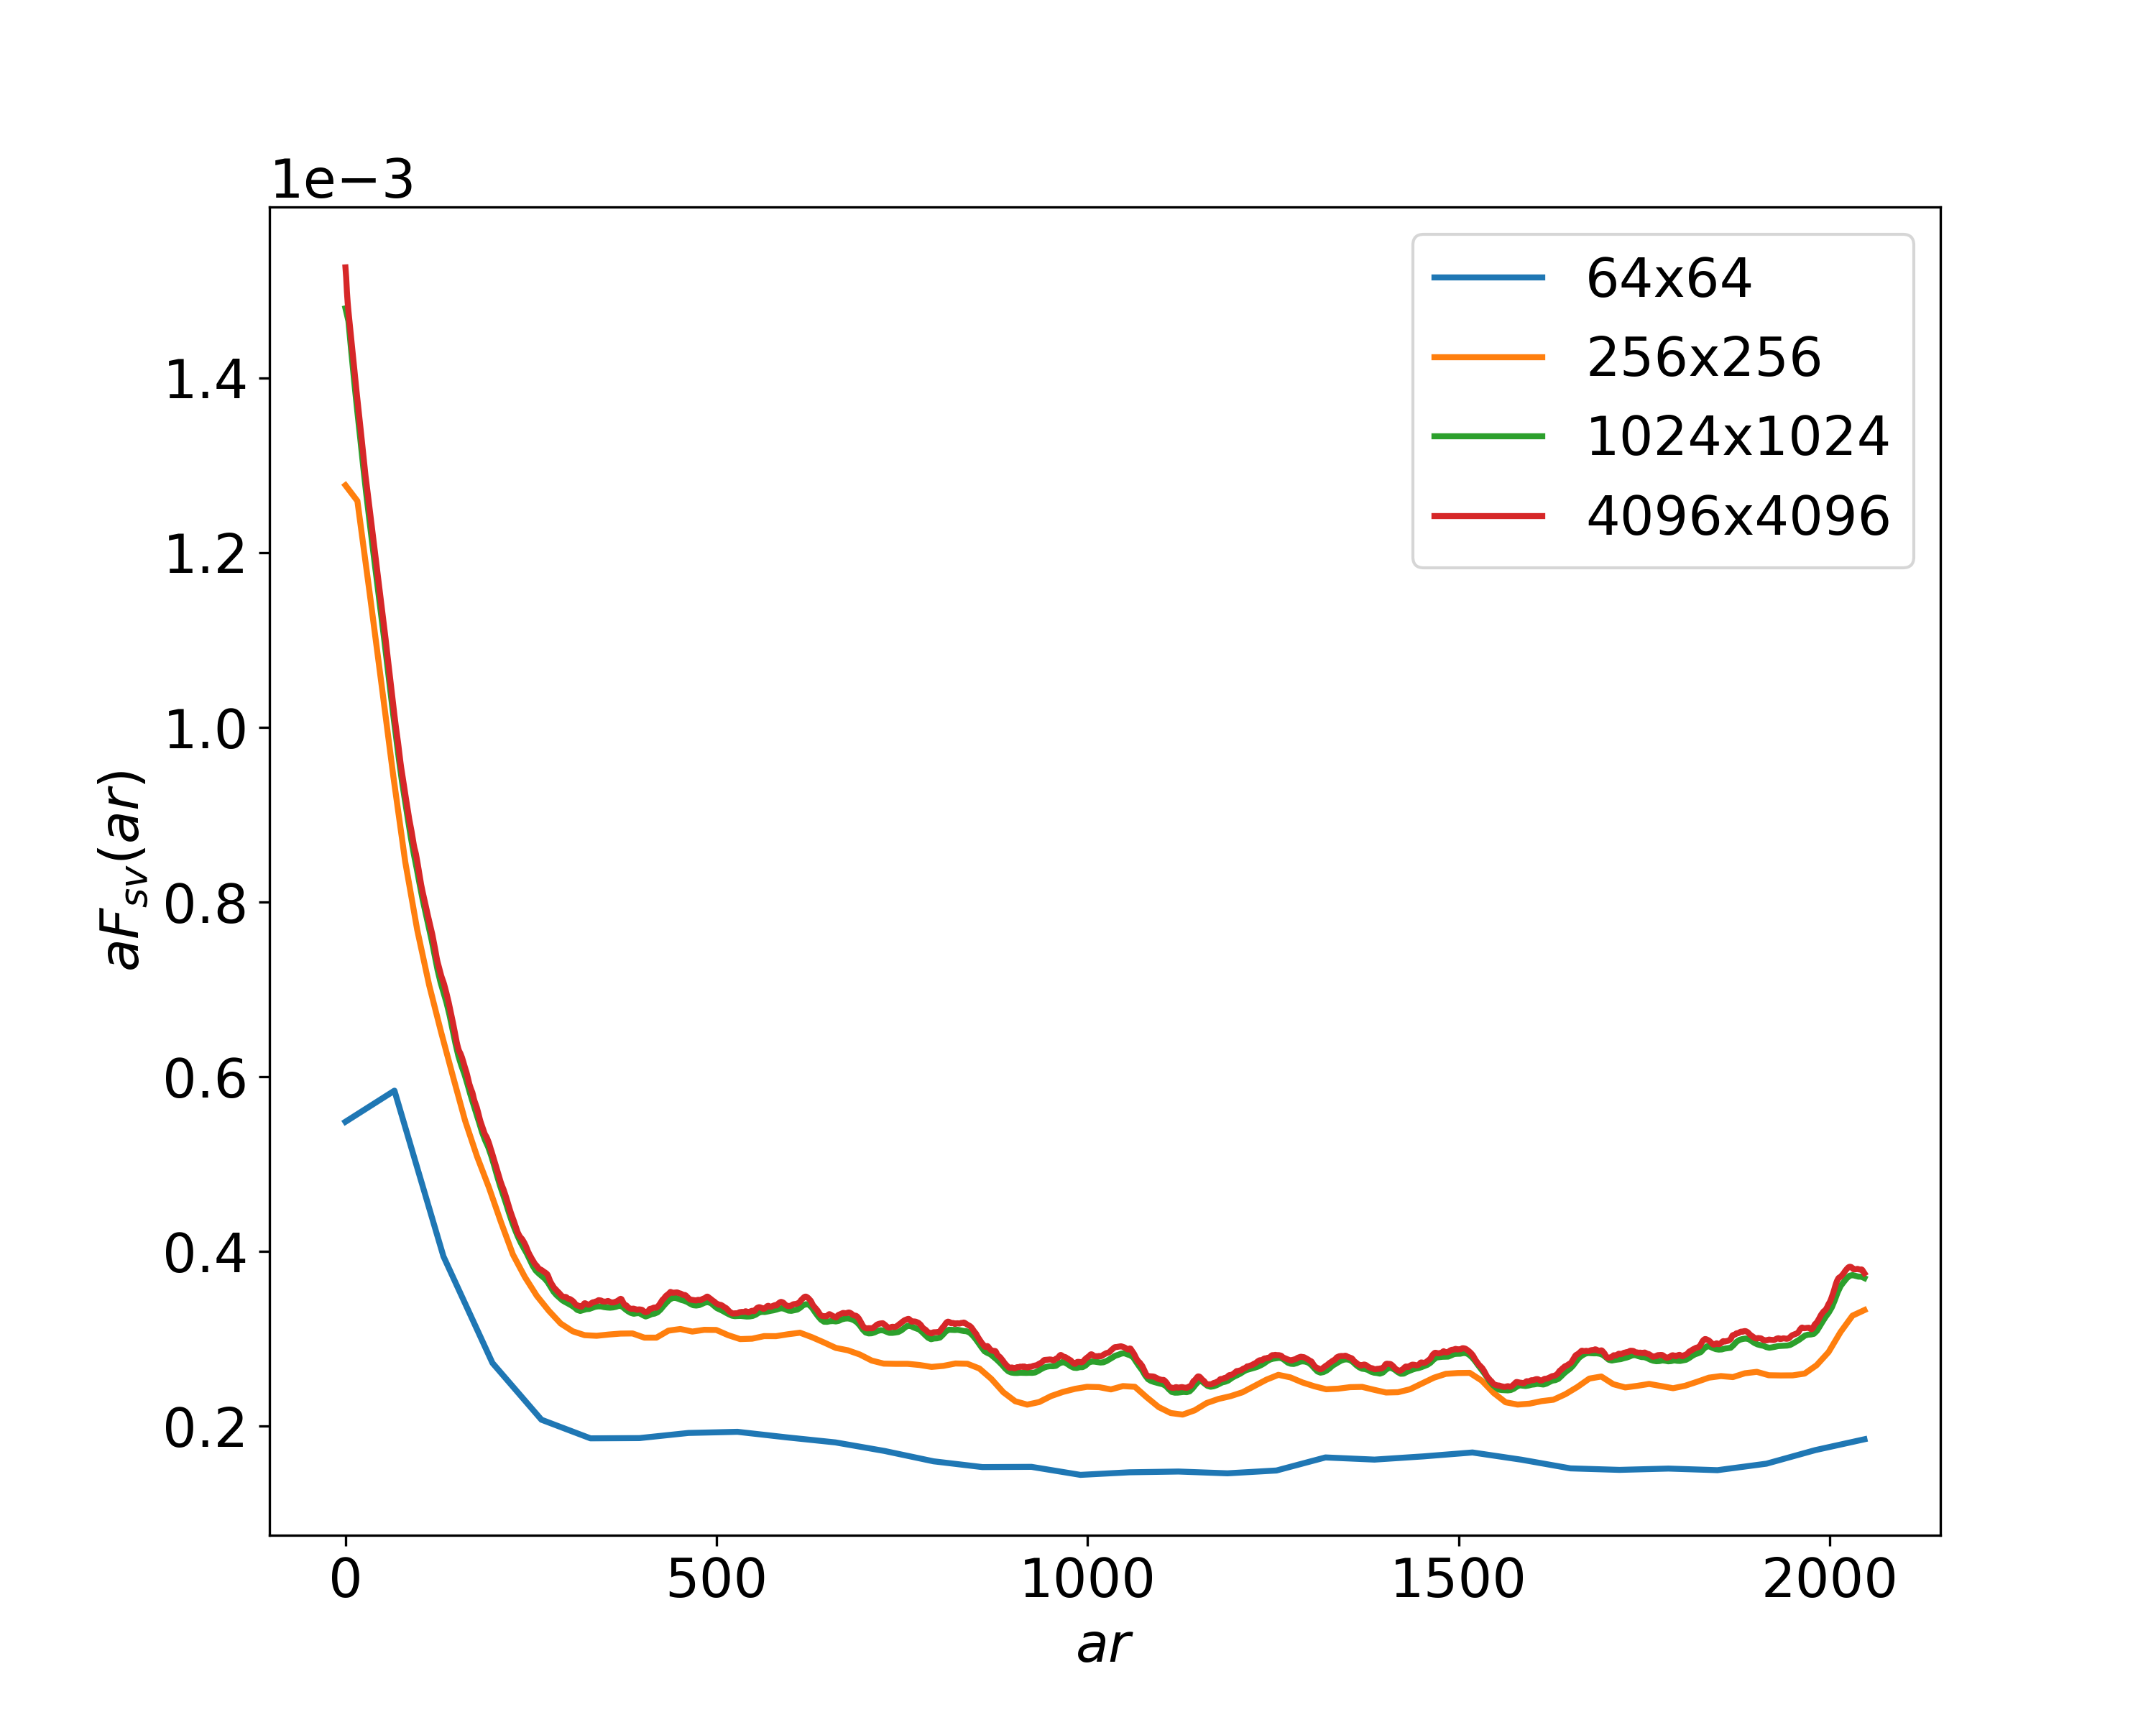
\includegraphics[width=0.475\linewidth]{images/plot-sv-noise.png}
    \label{fig:fsv-scaling-noise}}
    \caption[]{Surface-surface and surface-void correlation functions for
      thresholded value noise function sampled with different resolutions.}
    \label{fig:scaling-noise}
\end{figure*}

You can use resizing to obtain images of higher dimensionality and calculate
surface functions for resized images to get more accurate result. Because a
resized image becomes grayscale we use the following function as an indicator
for the void phase provided the void phase is marked as 0 in the original image:
\begin{equation*}
  I^{(void)}(x) = (1 - x)^{1.5}
\end{equation*}
Assuming an original small image is already two-phase we use the following
indicator function used to reduce multiphase image to two phases: $I(x) = x$
which is simply an identity function.

All interpolation methods are good for resizing purposes with exception of
nearest-neighbor. At \cref{fig:resized} you can see images of overlapped disks
with almost same surface-surface and surface-void functions. Correlation
functions for the original small image, resized image and recalculated?? image
are shown on \cref{fig:resized-cfs}.

\begin{figure*}[ht]
  \centering
  \subfigure[Resizing from $300 \times 300$ to $4000 \times 4000$ using bilinear
    interpolation]{
    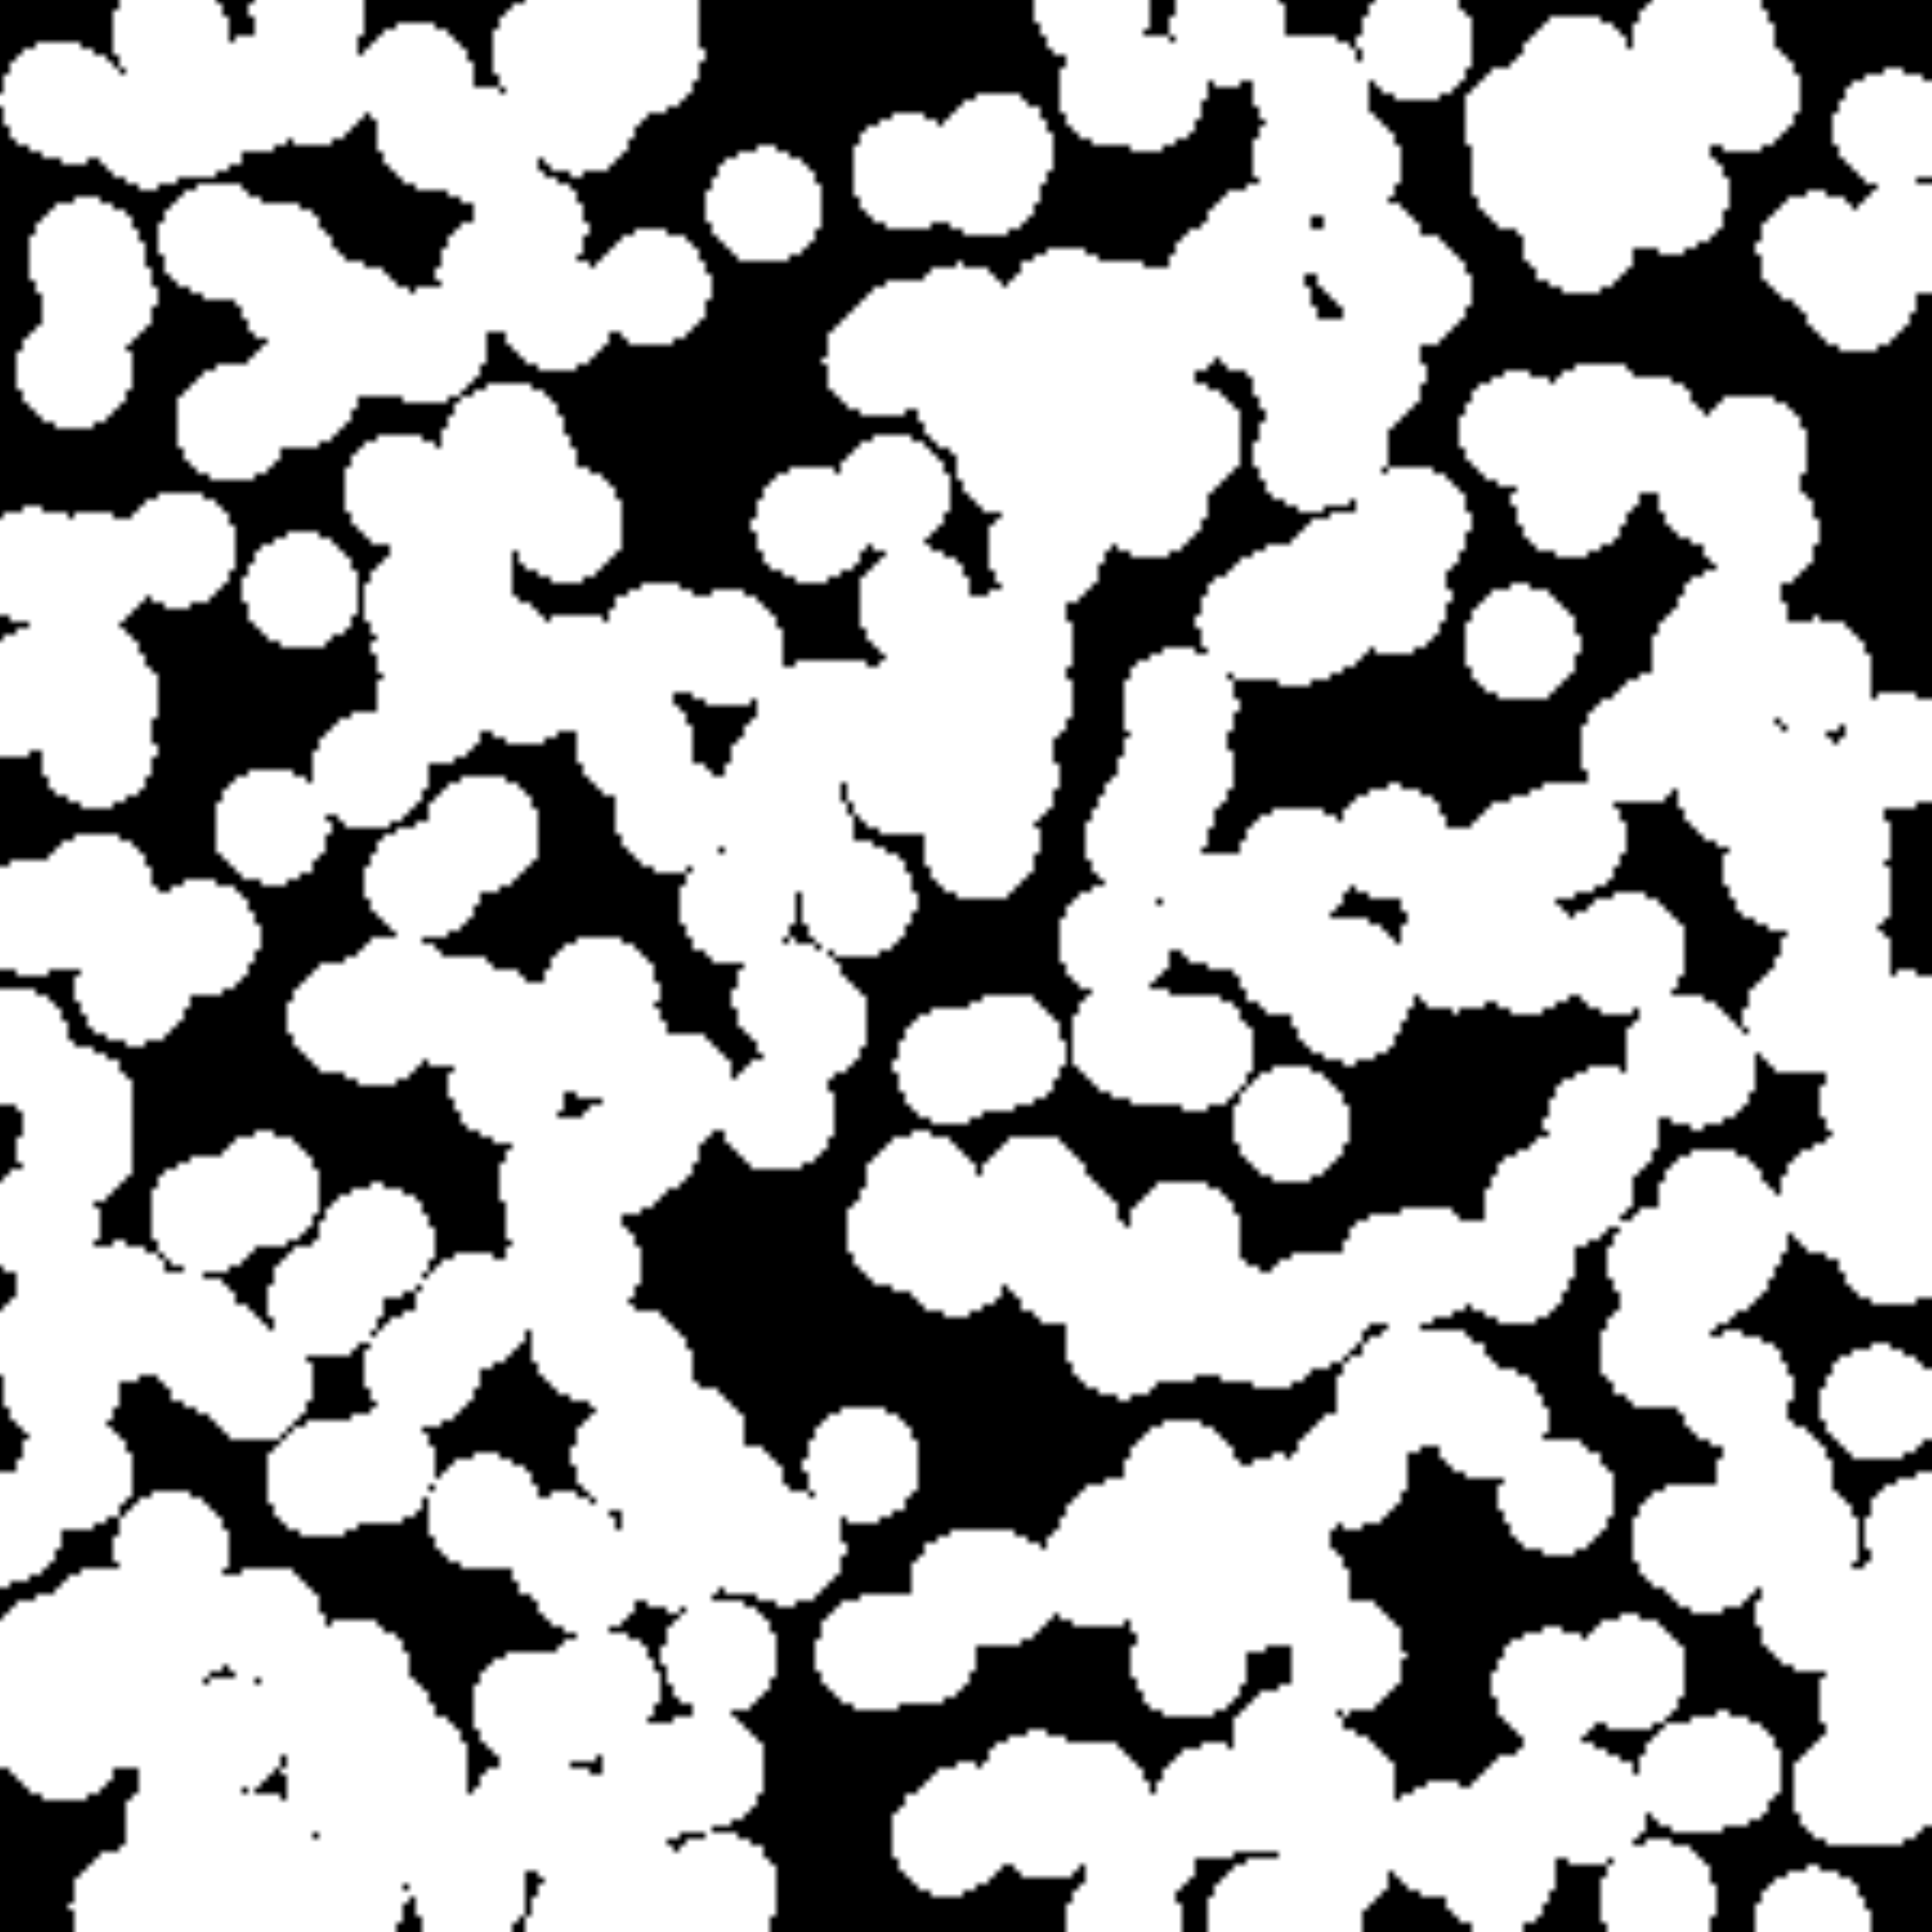
\includegraphics[width=0.45\linewidth]{resize-effects/disks-bilinear.png}
    \label{fig:resized-bilinear}}
  \hfill
  \subfigure[Recalculated??]{
    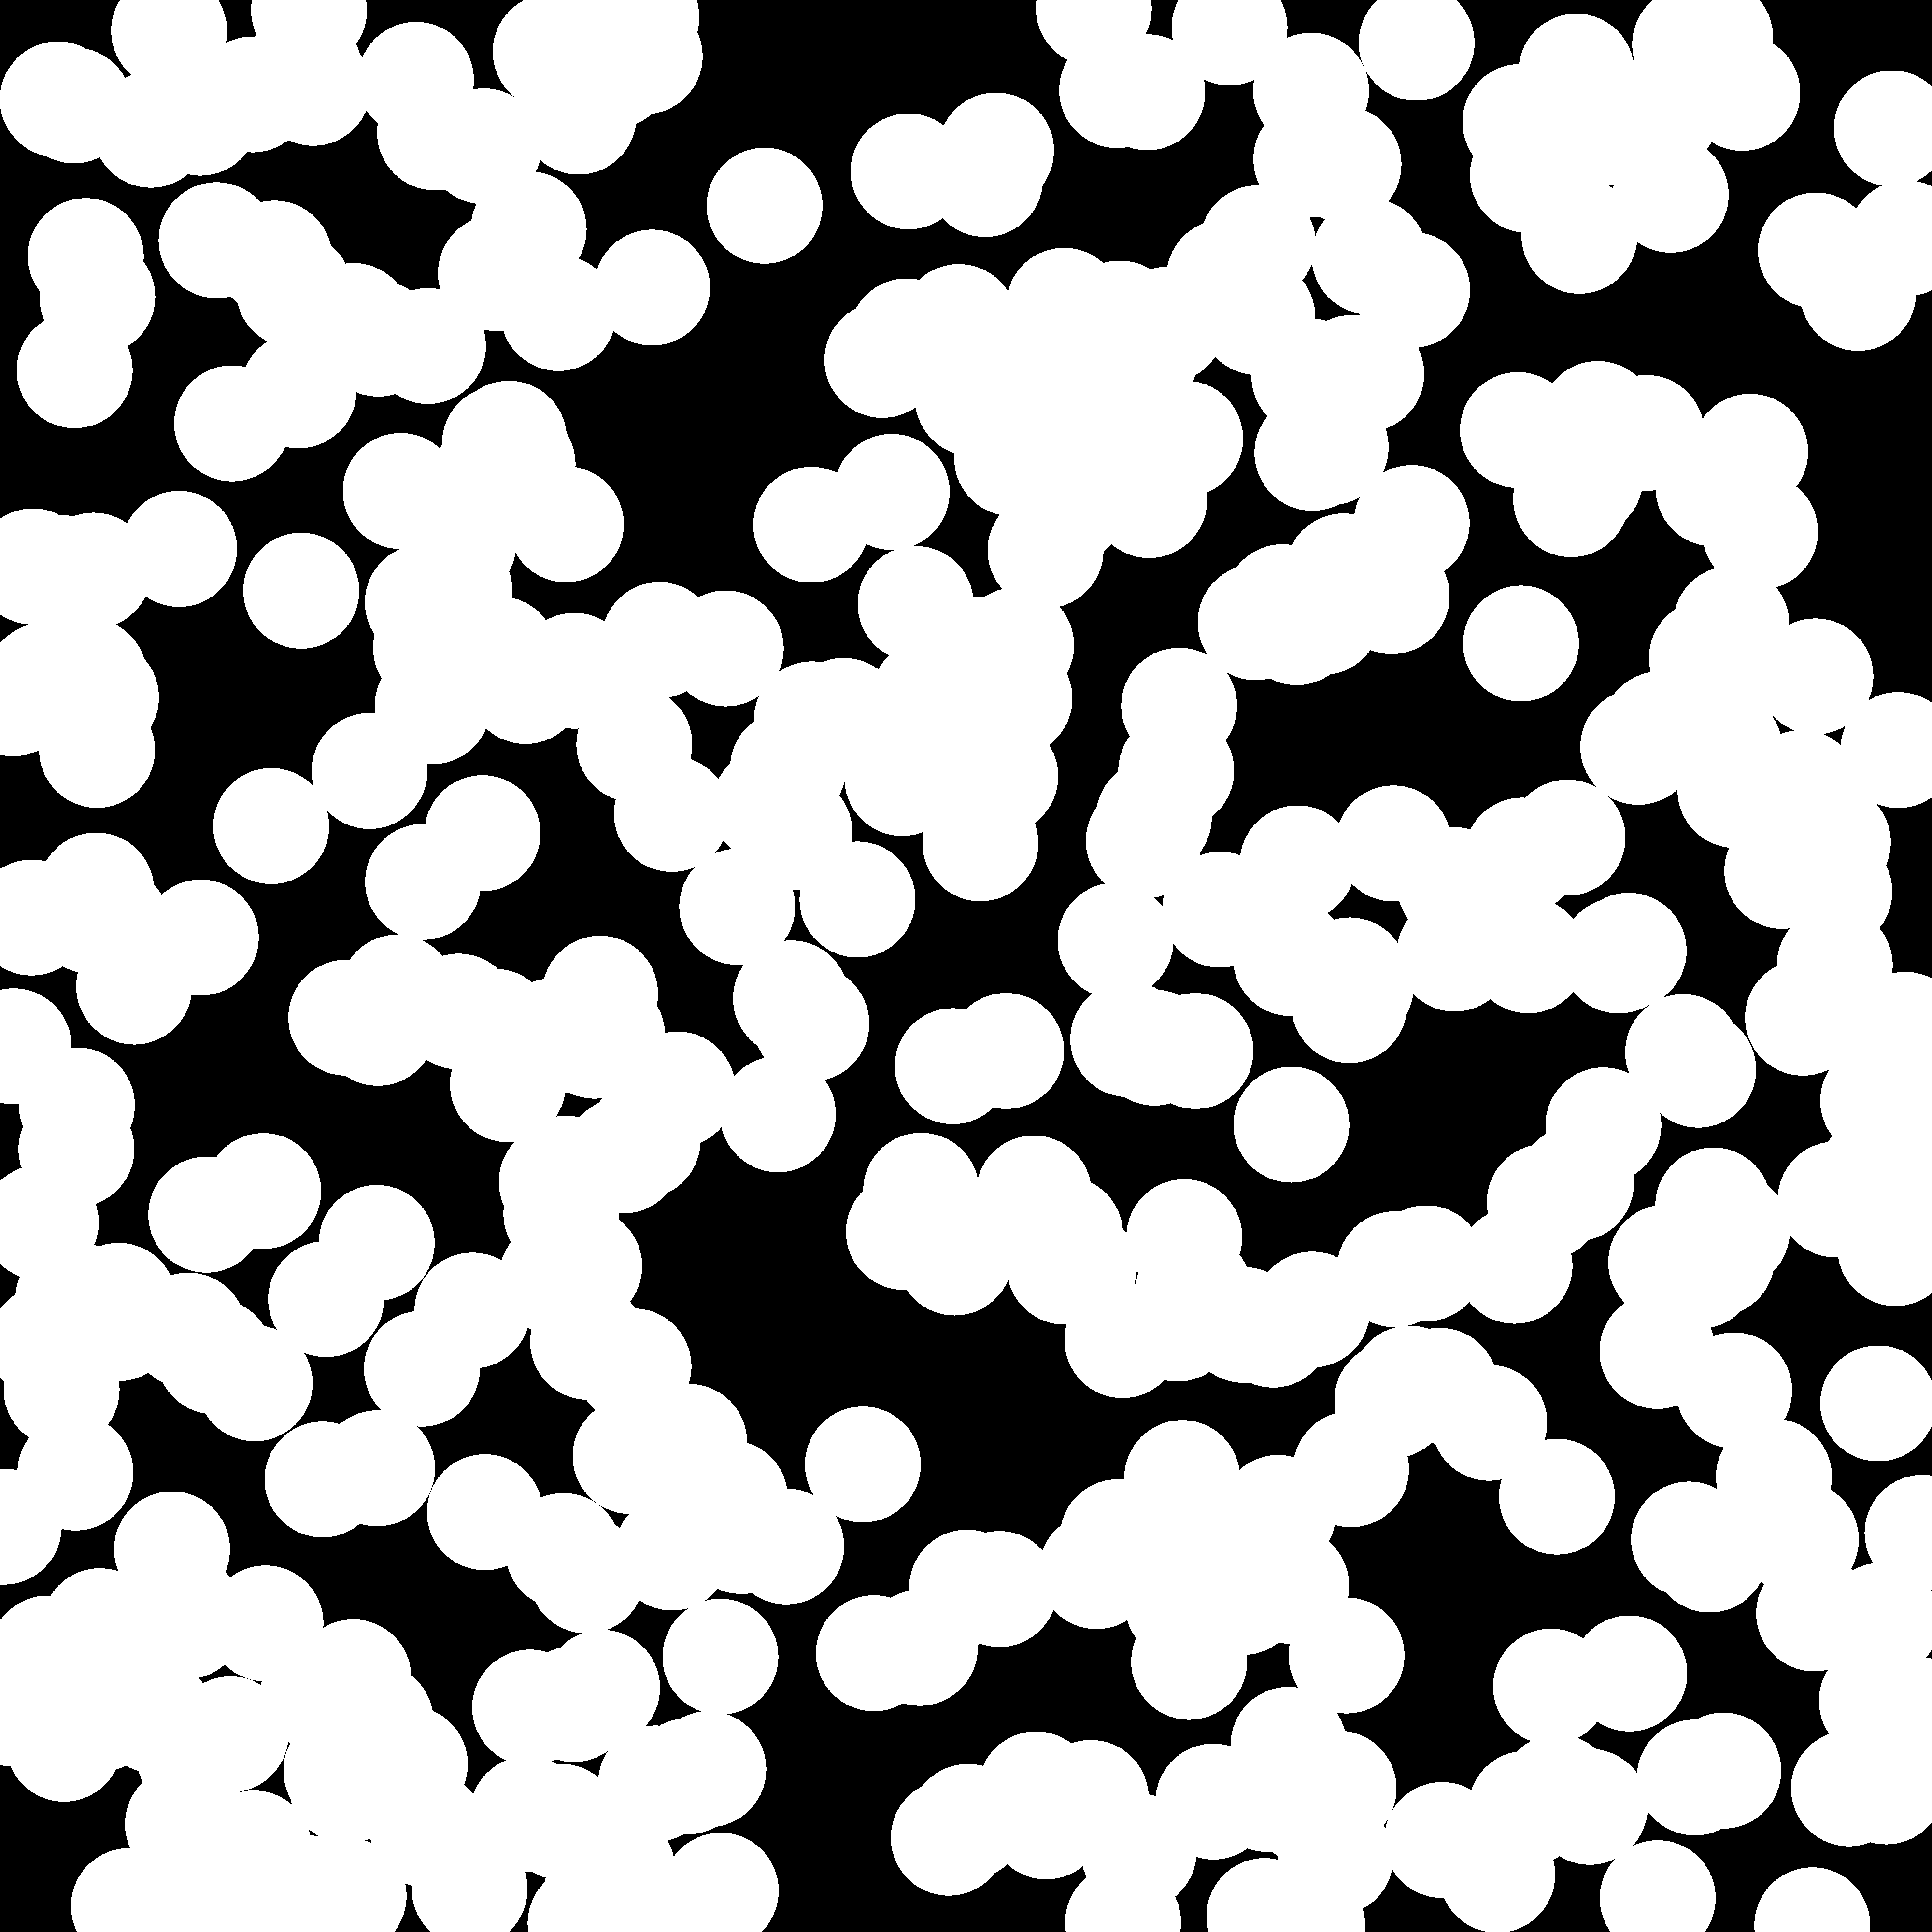
\includegraphics[width=0.45\linewidth]{resize-effects/disks-big.png}
    \label{fig:resized-true}}
  \caption[]{An example of images with almost equal correlation functions
    obtained using different methods.}
  \label{fig:resized}
\end{figure*}

\begin{figure*}[ht]
  \centering
  \subfigure[Surface-surface function]{
    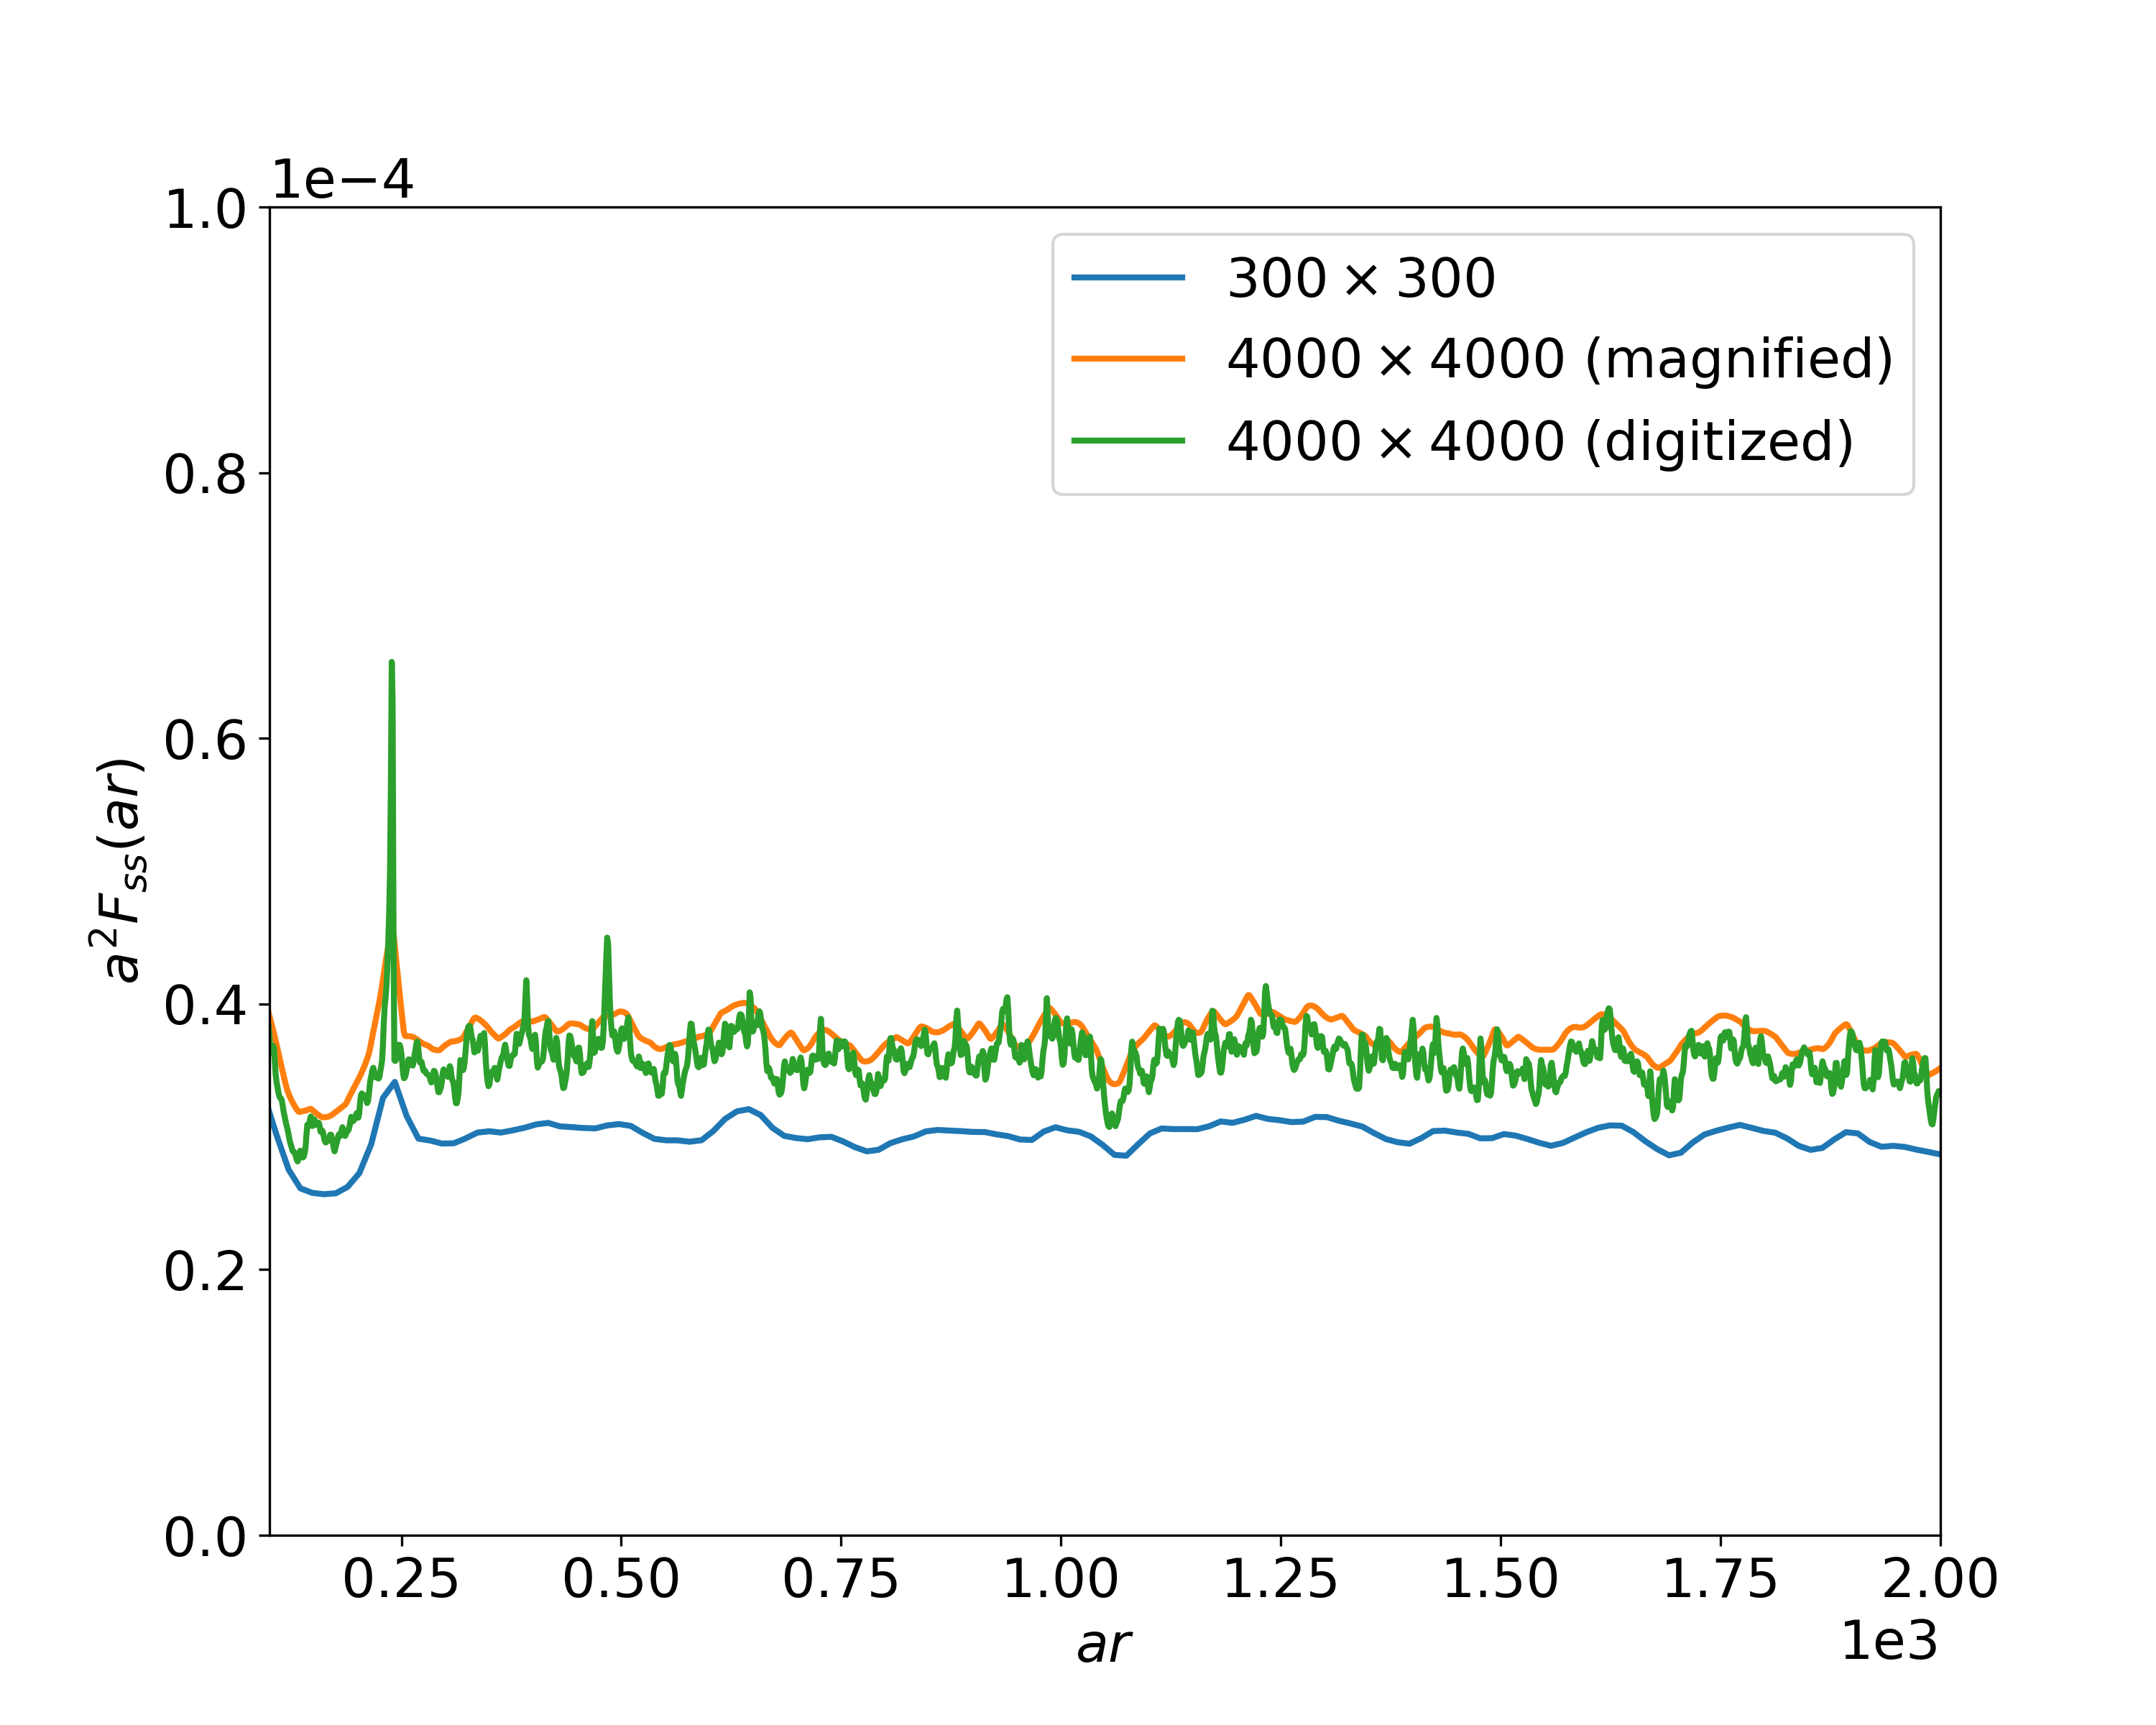
\includegraphics[width=0.45\linewidth]{resize-effects/surfsurf.png}
    \label{fig:resized-ss}}
  \hfill
  \subfigure[Surface-void function]{
    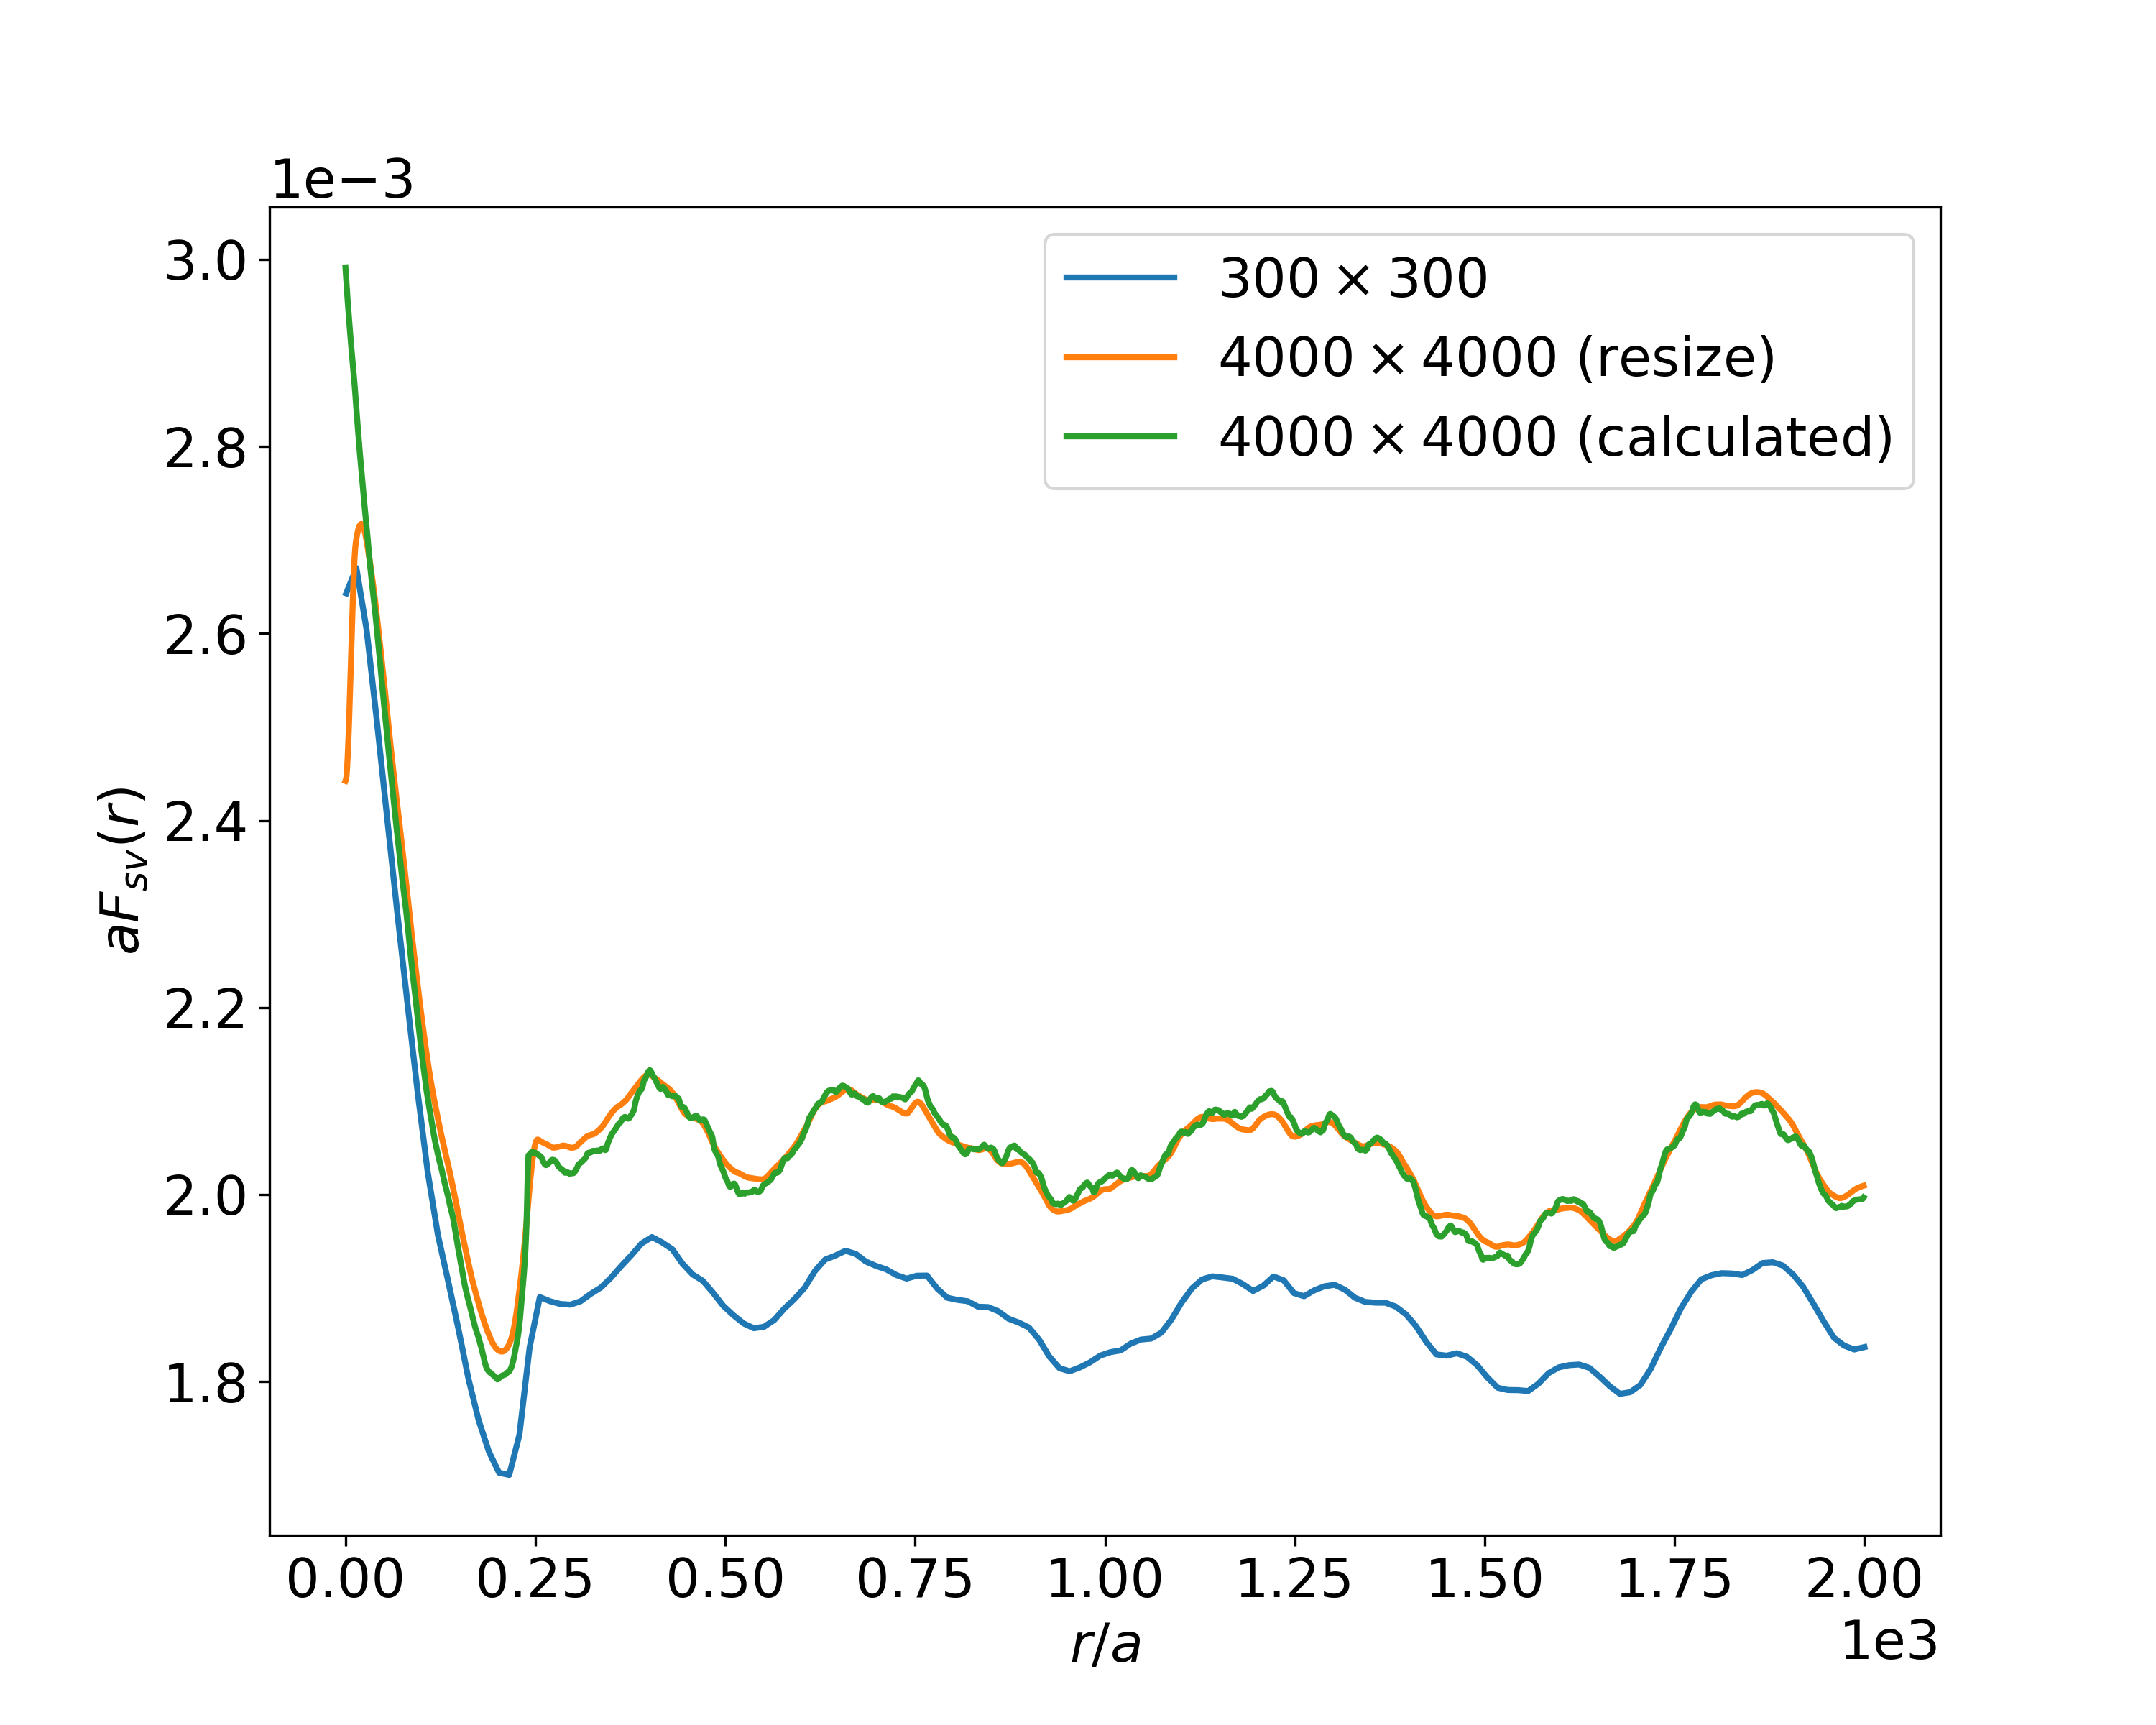
\includegraphics[width=0.45\linewidth]{resize-effects/surfvoid.png}
    \label{fig:resized-sv}}
  \caption[]{Correlation functions for image resized from $300 \times 300$ to
    $4000 \times 4000$ compared to correlation functions of the original image
    and recalculated?? image.}
  \label{fig:resized-cfs}
\end{figure*}

\subsection{The choice of method to extract the interface (gradient)}
\begin{figure}[ht]
  \centering
  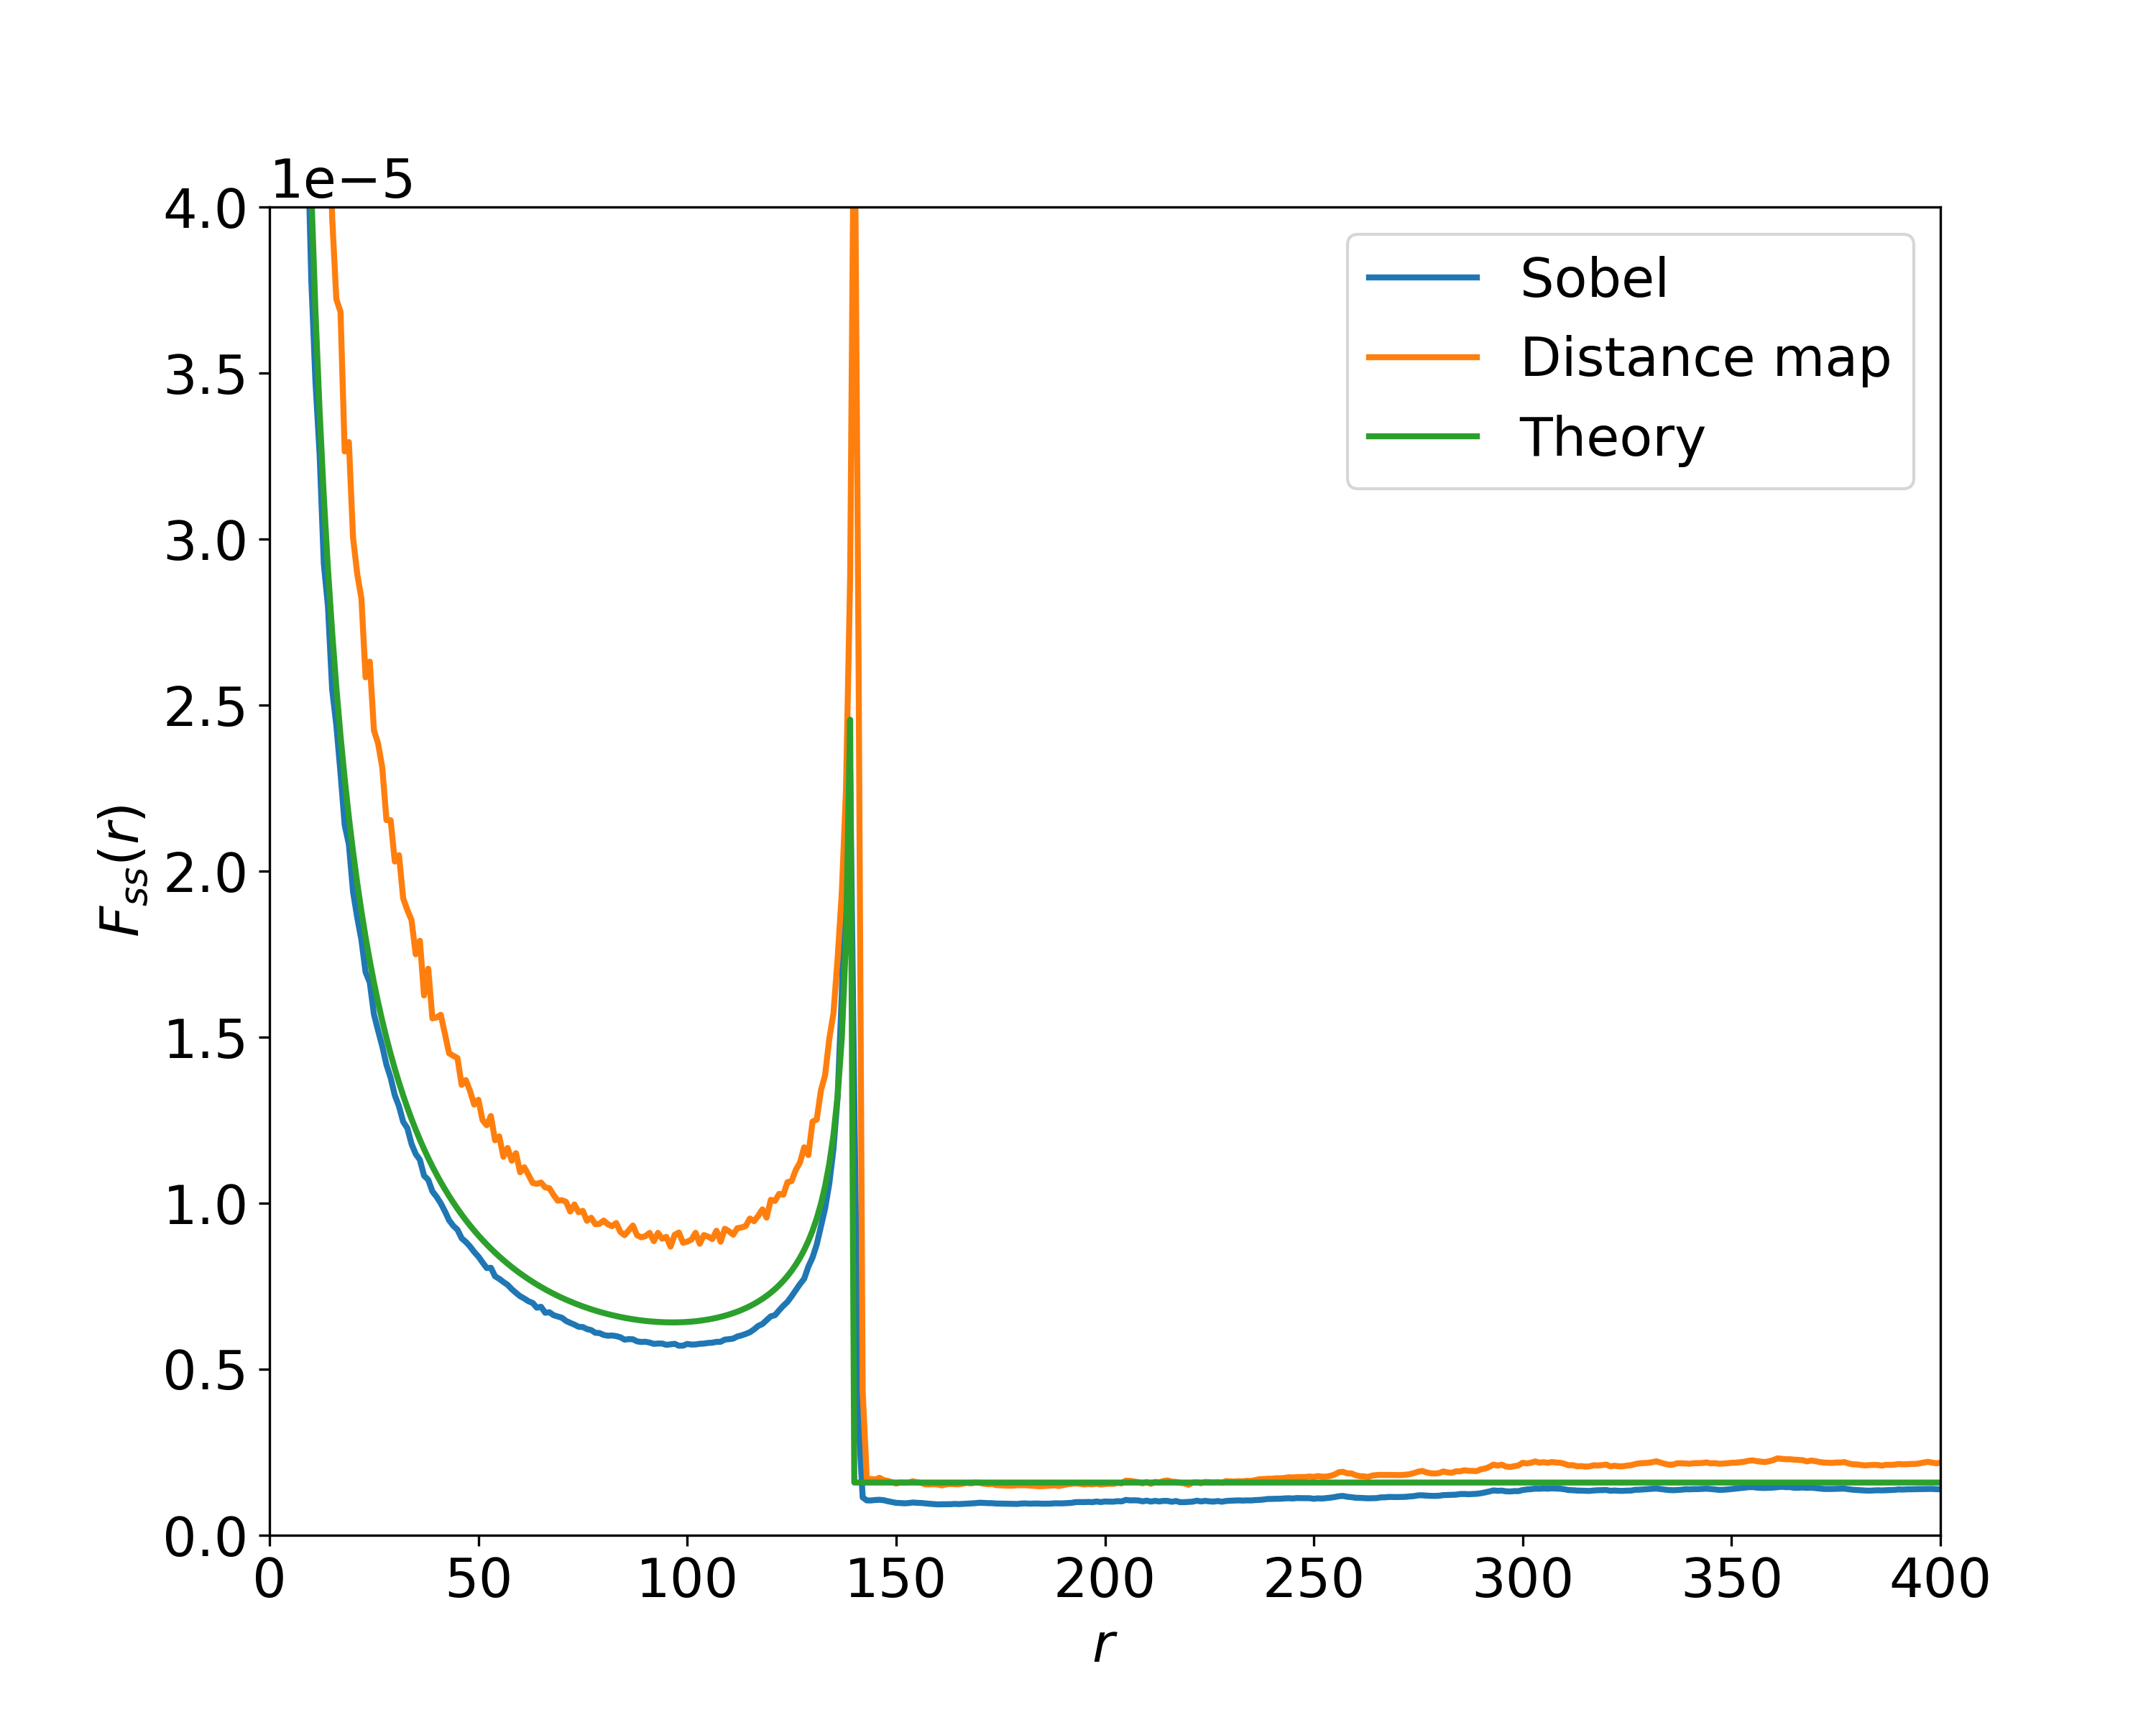
\includegraphics[width=0.99\linewidth]{images/sobel-vs-distance-map.png}
  \caption{Comparison of Sobel filter and distance map on high-resolution image (60 pixels per disk radius)}
  \label{fig:sobel-vs-distance-map}
\end{figure}

\begin{figure}[ht]
  \centering
  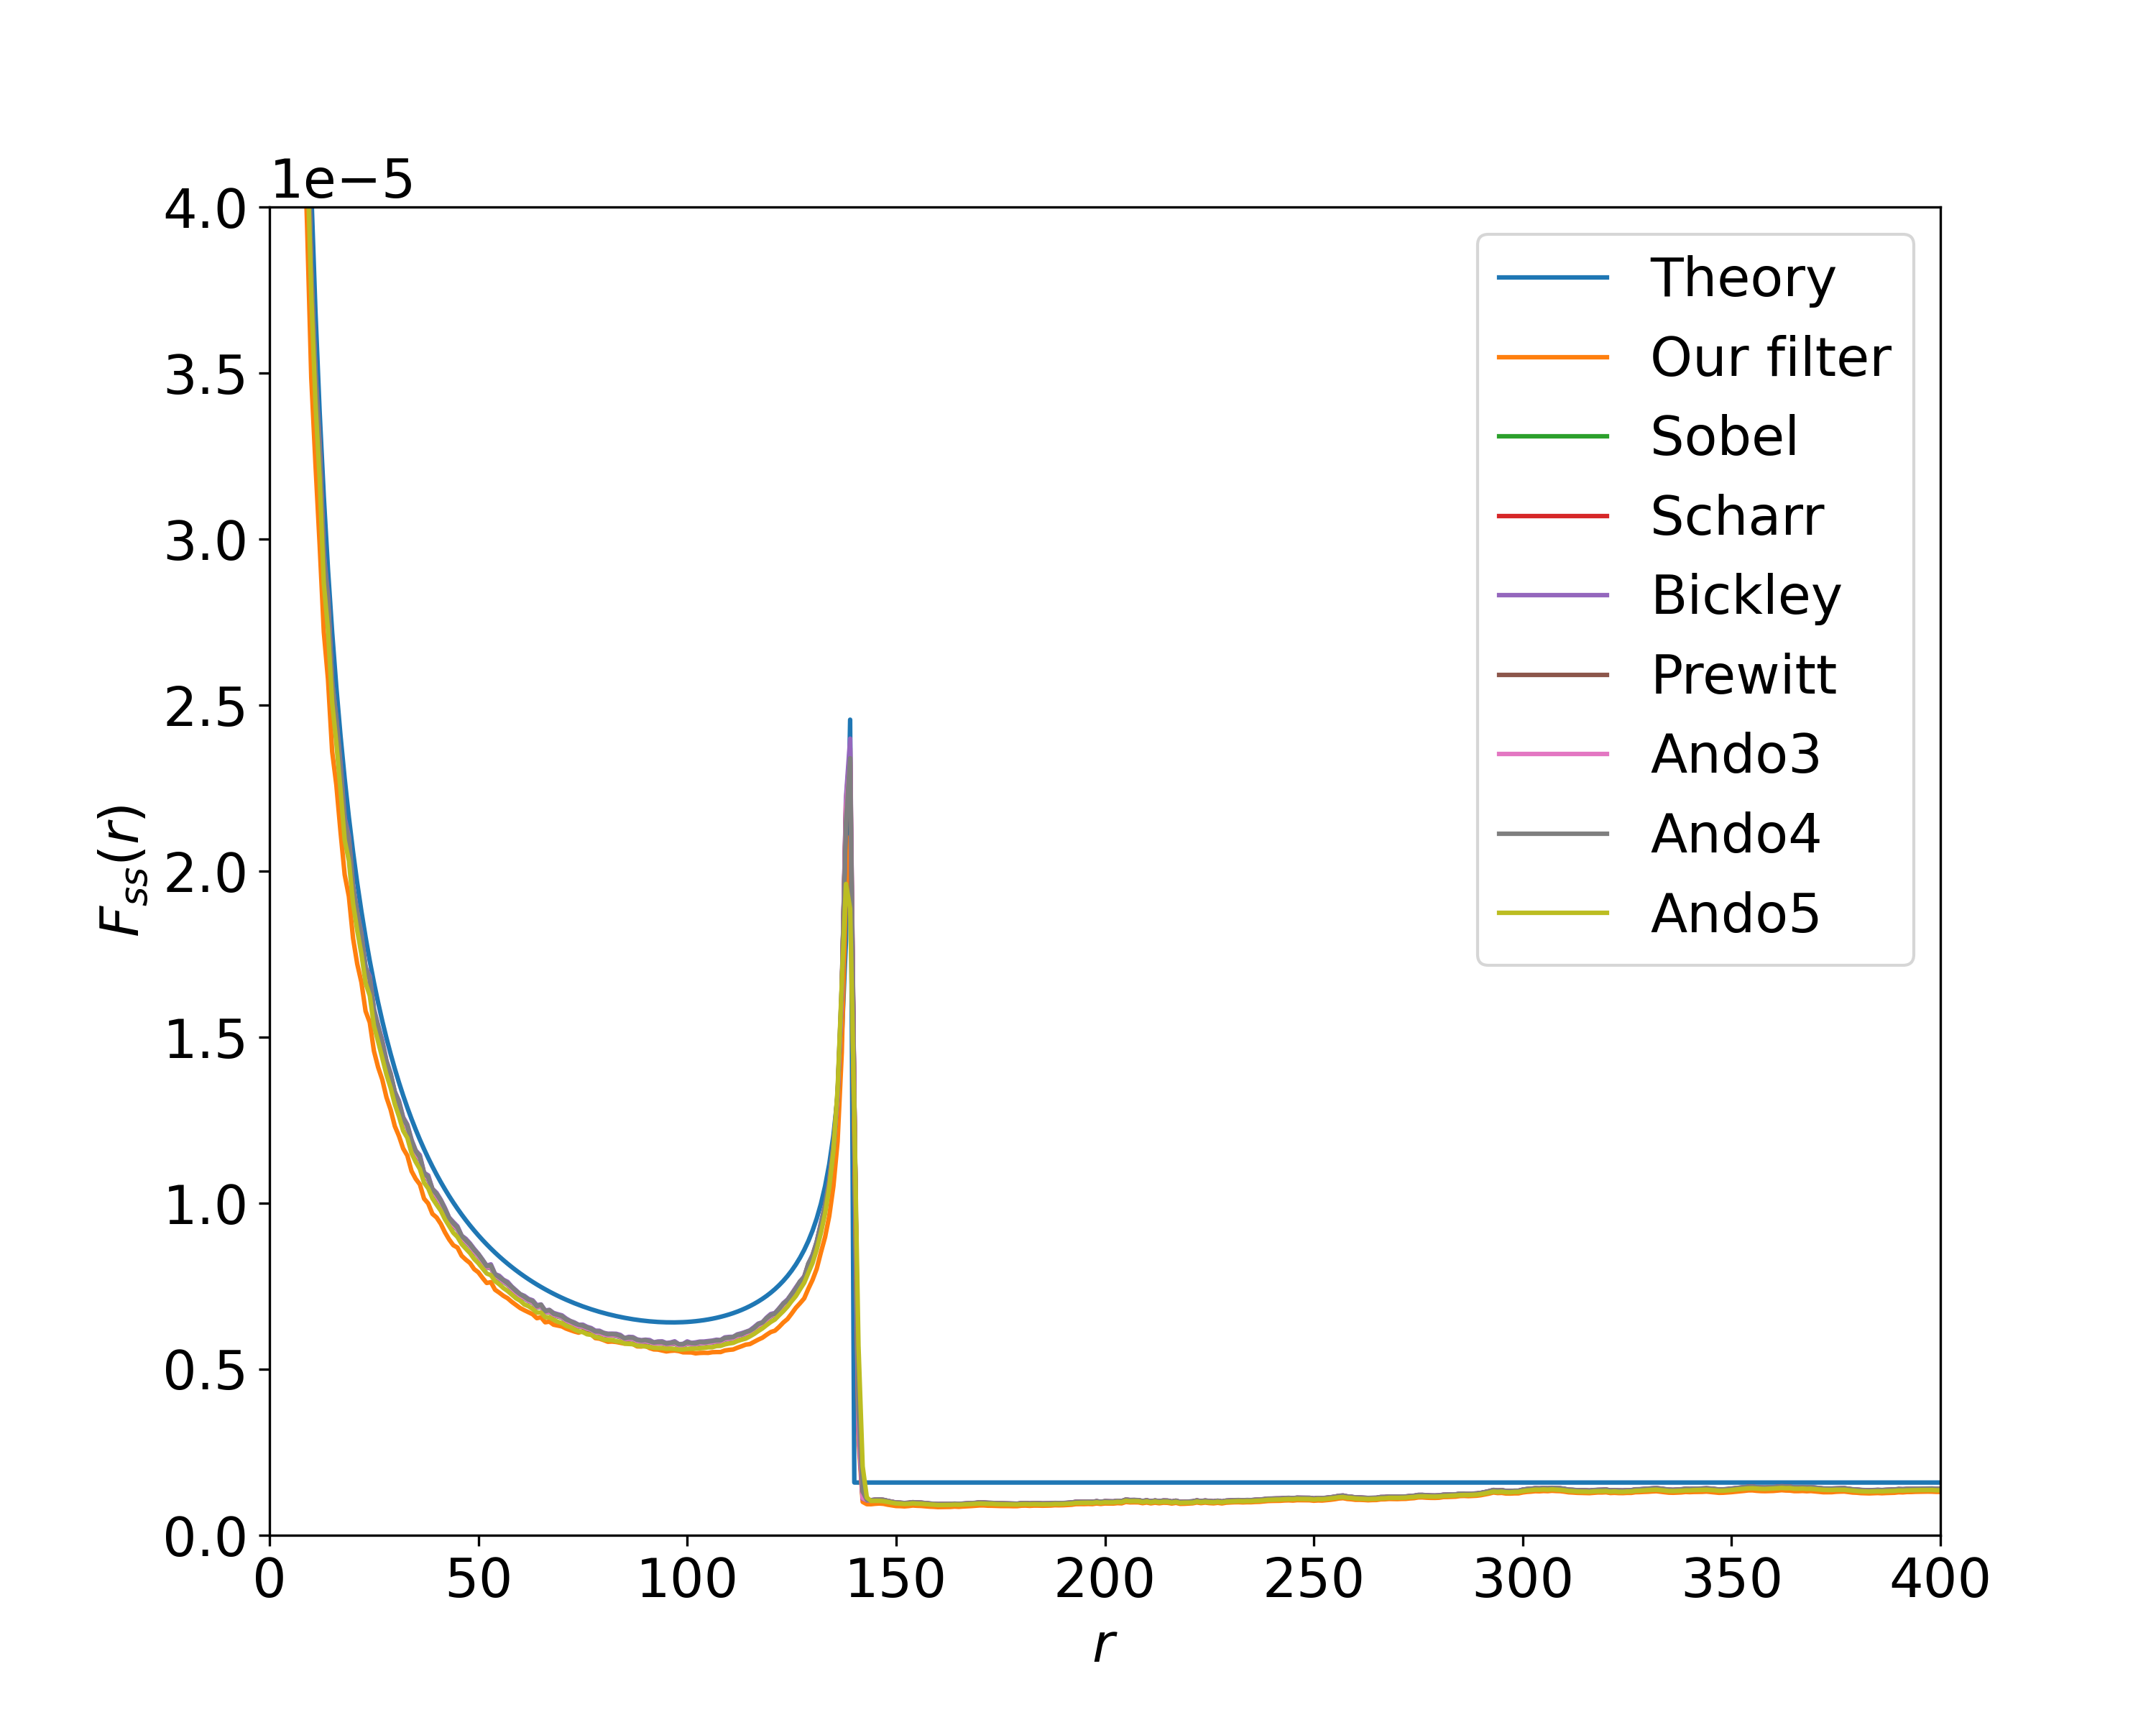
\includegraphics[width=0.99\linewidth]{images/kernels.png}
  \caption{Comparison of different filters.}
  \label{fig:kernels}
\end{figure}

Surface-surface function for overlapping disks
($R = 10,\ \lambda = 2 \cdot 10^{-3}$ on image with dimensions $1000 \times 1000$)
computed with different methods of interface extraction is shown on
\cref{fig:interface-extraction}. These methods include image filtering with
Sobel operator and interface extraction with distance map. When using distance
map both outer (\cref{eq:dist-outer}) and inner (\cref{eq:dist-inner})
interfaces are used to compute the correlation function. An average over the
last two functions is also shown. As you can see both methods -- distance map
and image filtering -- have an error compared to the analytical solution. If we
increase the radius of disks and the image resolution
($R = 70,\ \lambda = 3 \cdot 10^{-6}$ on image with dimensions $5000 \times 5000$)
we get the result as on \cref{fig:sobel-vs-distance-map}. In this case the image
filtering method achieved an analytical solution  while the distance map failed
to do so. This is why we advocate the use of image filtering to calculate
surface features.

There are many different kernels for evaluating gradients. We investigated:
Sobel, Ando, Sharr, Bickley and Prewitt filters. Their performance is almost the
same (\cref{fig:kernels}). The errors against the analytical solution are
close. And different kernels work better for different images. Therefore, it is
difficult to recommend a specific kernel.

\subsection{Criterion for accurate evaluation of surface CFs from discrete images}
\label{sec:crit}
Let us define one-dimensional forward ($F$) and inverse ($F^{-1}$) Fourier
transforms as:
\begin{align}
  \hat{f}(z) &= F[f](z) = \frac{1}{\sqrt{2\pi}}\int_{-\infty}^{\infty} f(x)
  e^{-i\pi xz} dx \label{eq:fourier-forward} \\
  f(x) &= F^{-1}[\hat{f}](z) = \frac{1}{\sqrt{2\pi}}\int_{-\infty}^{\infty} \hat{f}(z)
  e^{i\pi xz} dz \label{eq:fourier-backward}
\end{align}

Here $f(x)$ and $\hat{f}(z)$ can be thought of as representations of a signal in
the time domain and the frequency domain, respectively. Both equations
\cref{eq:fourier-forward} and \cref{eq:fourier-backward} preserve norm on $L_2$:
$(f, f) = (\hat{f}, \hat{f})$. It is said that Fourier transform preserves
``energy'' of the signal. According to Riemann-Lebesgue lemma \cite{HilbertSpaces}
energy of any signal ``concentrates'' around low frequencies. A measure of how
much energy concentrated in low frequencies (for some definition of low
frequencies) is a key to the understanding of the problem of correctness of our
method. The Shannon sampling theorem \cite{HilbertSpaces} states that it is
possible to reconstruct a band-limited signal $f(x)$ whose frequencies lie in
the range $[0, f]$ from a sequence of samples $\left\{f_n\right\}$ if the
sampling rate is no less than $2f$. We introduce a parameter $C_a$:
\begin{align*}
  f_0(x) &= f(x) - \langle f(x) \rangle \\
  C_a &= \frac{\int_{-a\omega}^{a\omega} |\hat{f_0}(z)|^2 dz}{\int_{-\omega}^{\omega} |\hat{f_0}(z)|^2 dz}
\end{align*}
where $\omega = 2\pi f$ and $\langle f(x) \rangle$ is the mean value of $f(x)$
over its domain. The criterion for correctness is then:
\begin{equation*}
  C_a > 1 - \xi
\end{equation*}
for some $a$ and $\xi$. This criterion tells us exactly how much energy in
$f_0(x)$ is concentrated in a low frequency range $[0, af]$ compared to the
whole range $[0, f]$. In our work we propose $a = 0.5$ and $\xi = 0.07$ as
a strict criterion which is based on results of \cref{sec:comparison}. For the
images of Poisson disks from \cref{fig:scaling} their discretizations and
$C_{0.5}$ are shown in \cref{fig:disks-res}. We immediately observe that the
image with resolution $4096 \times 4096$ has surface CFs very close to
analytical solution and satisfy our  $C_{0.5}$ criterion perfectly. The other
three downscaled images fail to satisfy the criterion. After looking at
\cref{fig:scaling} and \cref{fig:disks-res} we can claim that the criterion
correctly selects images which are suitable for calculation of the correlation
functions. The criterion $C_{0.5}$ decays fast with the decline in image
resolution as shown in \cref{fig:crit-plot}.

\begin{figure}[ht]
  \centering
  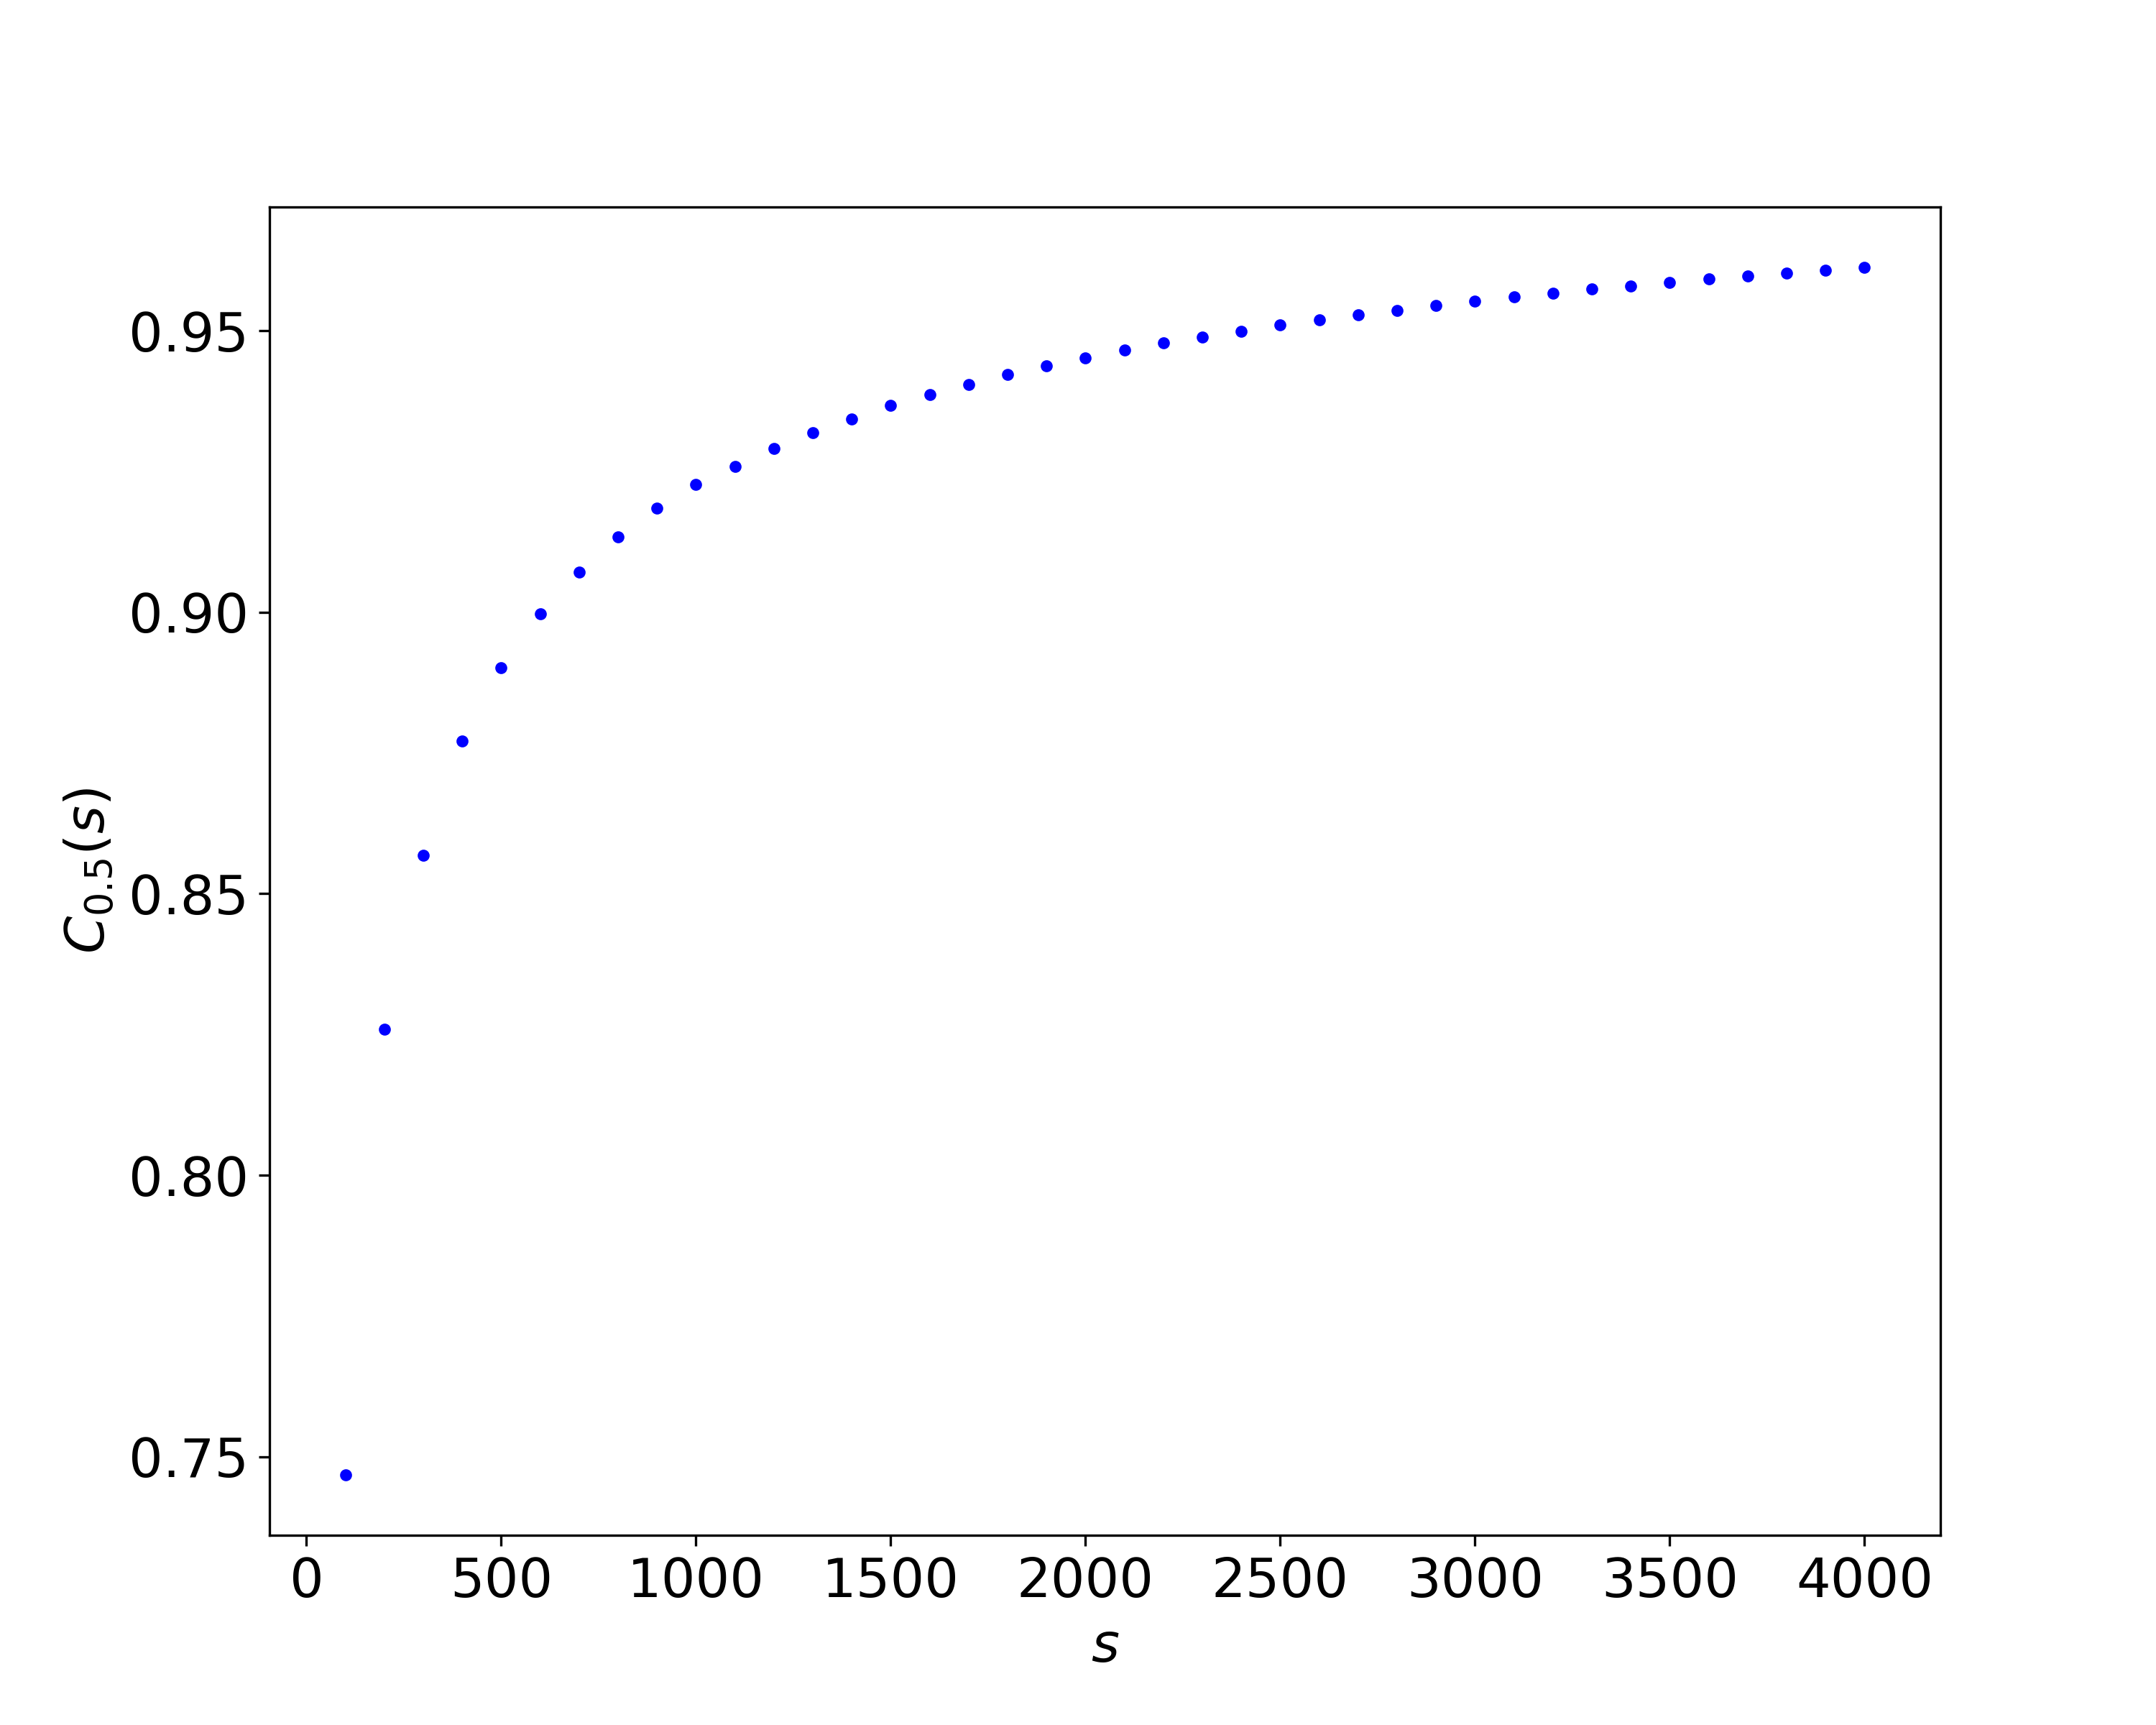
\includegraphics[width=0.9\linewidth]{images/plot-criterion.png}
  \caption[]{Decay of criterion $C_{0.5}$ as a function of the size $s$ of
    the downscaled image.}
  \label{fig:crit-plot}
\end{figure}

\begin{figure*}[t]
  \centering
  \subfigure[Resolution $4096 \times 4096$, disk radius 61.44 pixels, $C_{0.5} = 0.9593$]{
    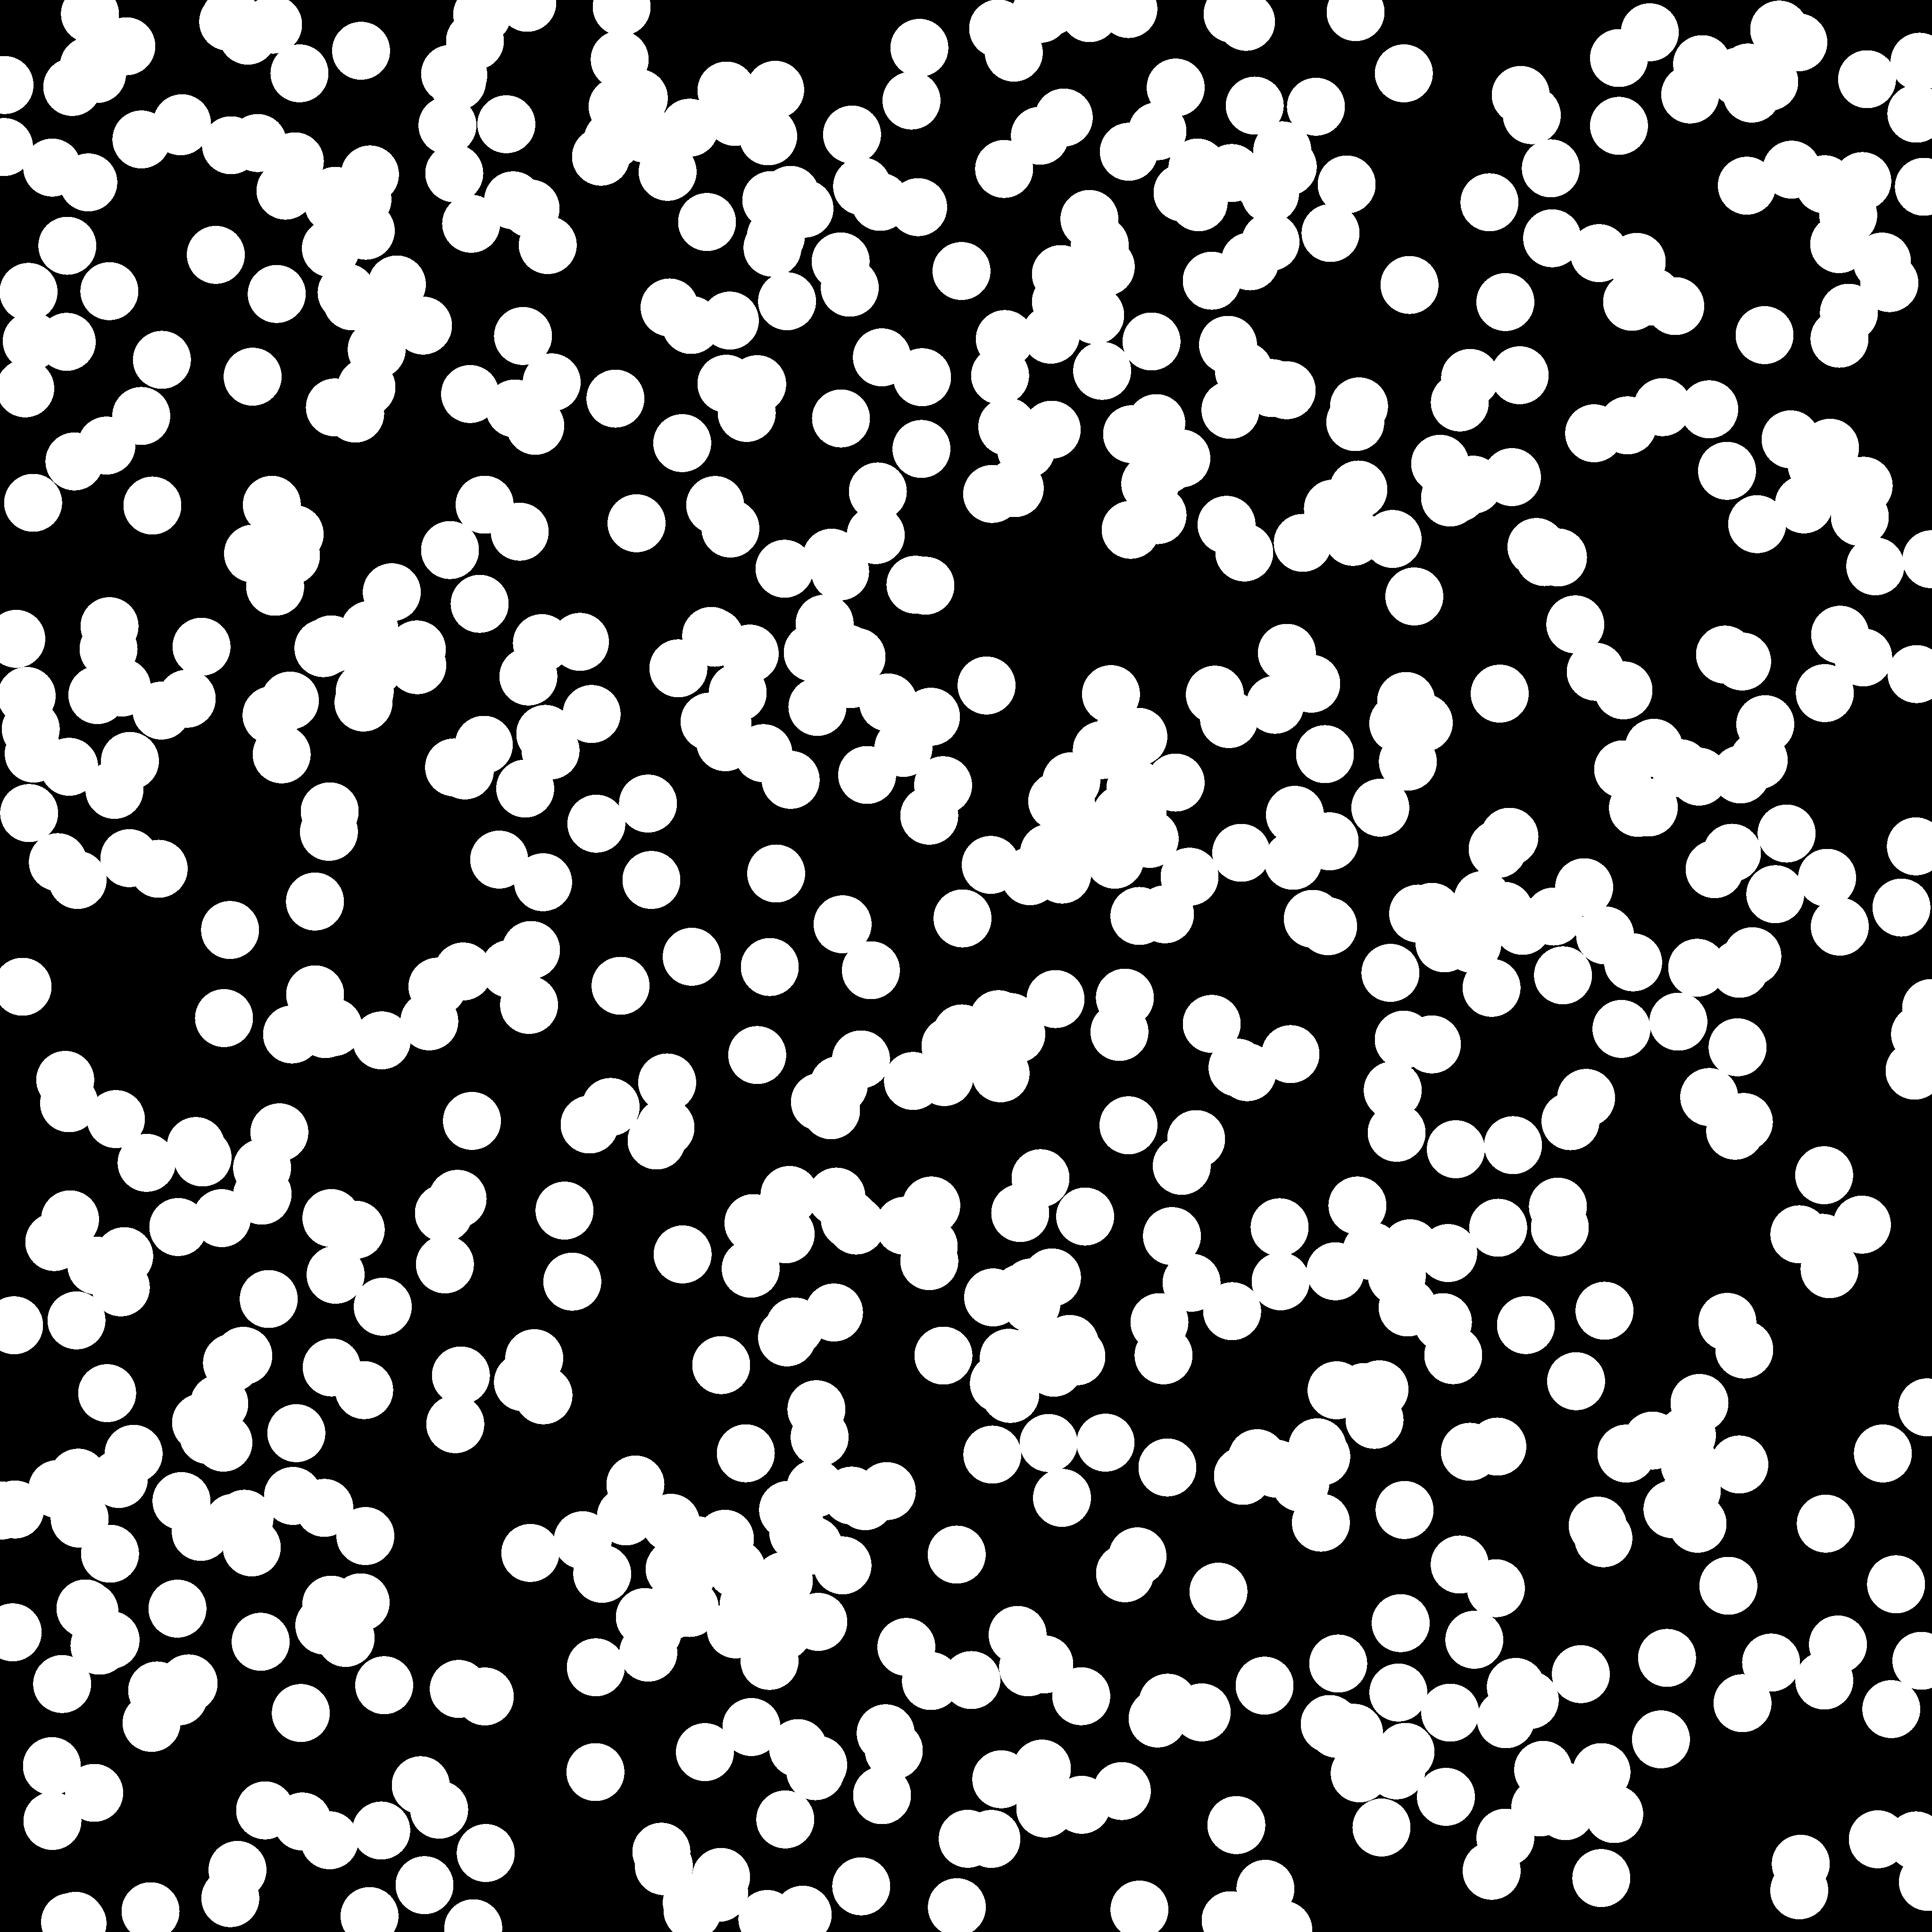
\includegraphics[width=0.475\linewidth]{images/disks-0015-5e-5-4096.png}
    \label{fig:disks-4096}}
  \hfill
  \subfigure[Resolution $1024 \times 1024$, disk radius 15.36 pixels, $C_{0.5} = 0.9185$]{
    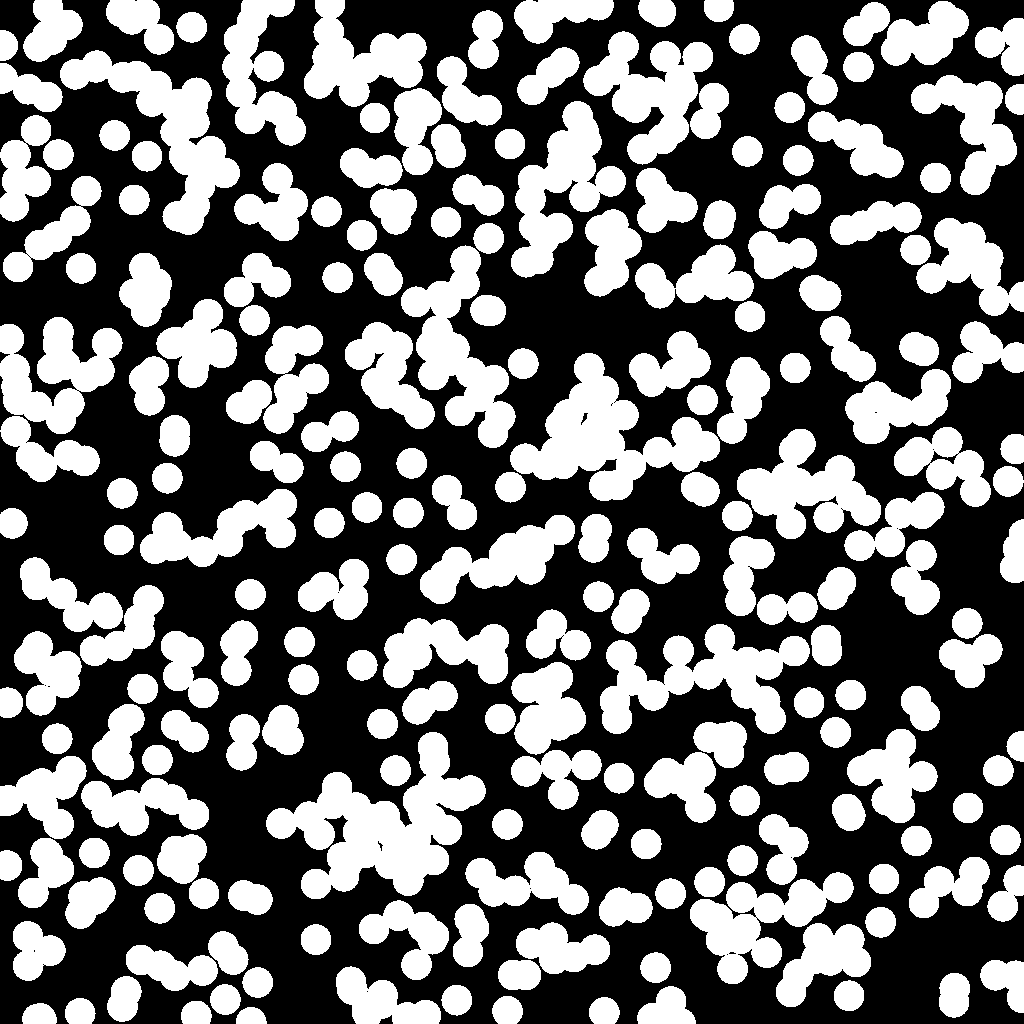
\includegraphics[width=0.475\linewidth]{images/disks-0015-5e-5-1024.png}
    \label{fig:disks-1024}}
  \vskip\baselineskip
  \subfigure[Resolution $256 \times 256$, disk radius 3.84 pixels, $C_{0.5} = 0.8356$]{
    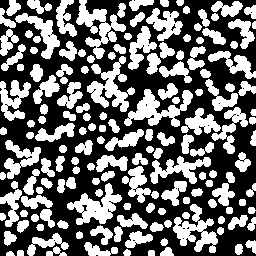
\includegraphics[width=0.475\linewidth]{images/disks-0015-5e-5-256.png}
    \label{fig:disks-256}}
  \hfill
  \subfigure[Resolution $64 \times 64$, disk radius 0.96 pixels, $C_{0.5} = 0.6549$]{
    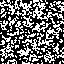
\includegraphics[width=0.475\linewidth]{images/disks-0015-5e-5-64.png}
    \label{fig:disks-64}}
  \caption[]{The influence of imaging resolution on the quality of surface
    correlation functions computations (as shown in \cref{fig:scaling}) based on
    the criterion $C_{0.5}$.}
  \label{fig:disks-res}
\end{figure*}

\subsection{Application to binary images of porous media}
\label{sec:application}
After the verification of our computational approach based on analytical
solution and establishing the criterion $C_{0.5}$ we now have enough tools to
evaluate surface CFs for different porous media images, including real XCT and
SEM images.

For demonstration purposes, we computed correlation functions for three
sandstone and three carbonate samples with dimensions
$500 \times 500 \times 500$ (\cref{fig:real-data}) all of which satisfy our
$C_{0.5}$ criterion. The result can be seen on \cref{fig:real-data-plots}.

There are examples of bad images which do not pass our criterion on
\cref{fig:real-bad}.

\begin{figure*}[t]
  \centering
  \subfigure[Sandstone 1, $C_{0.5} = 0.938$]{
    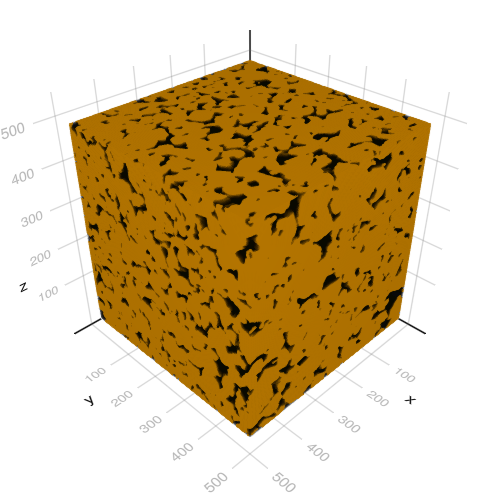
\includegraphics[width=0.3\linewidth]{images/sandstone1.png}
    \label{fig:sandstone1}}
  \hfill
  \subfigure[Sandstone 2, $C_{0.5} = 0.937$]{
    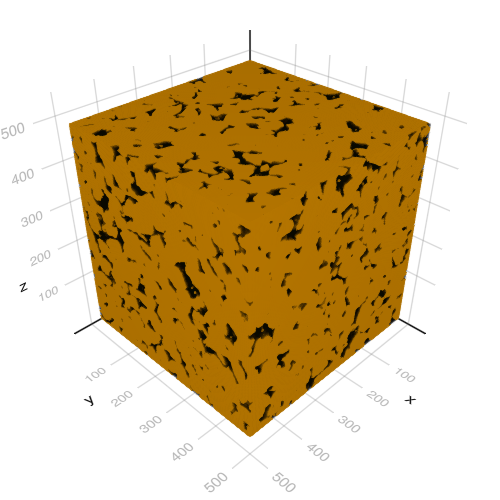
\includegraphics[width=0.3\linewidth]{images/sandstone2.png}
    \label{fig:sandstone2}}
  \hfill
  \subfigure[Sandstone 3, $C_{0.5} = 0.939$]{
    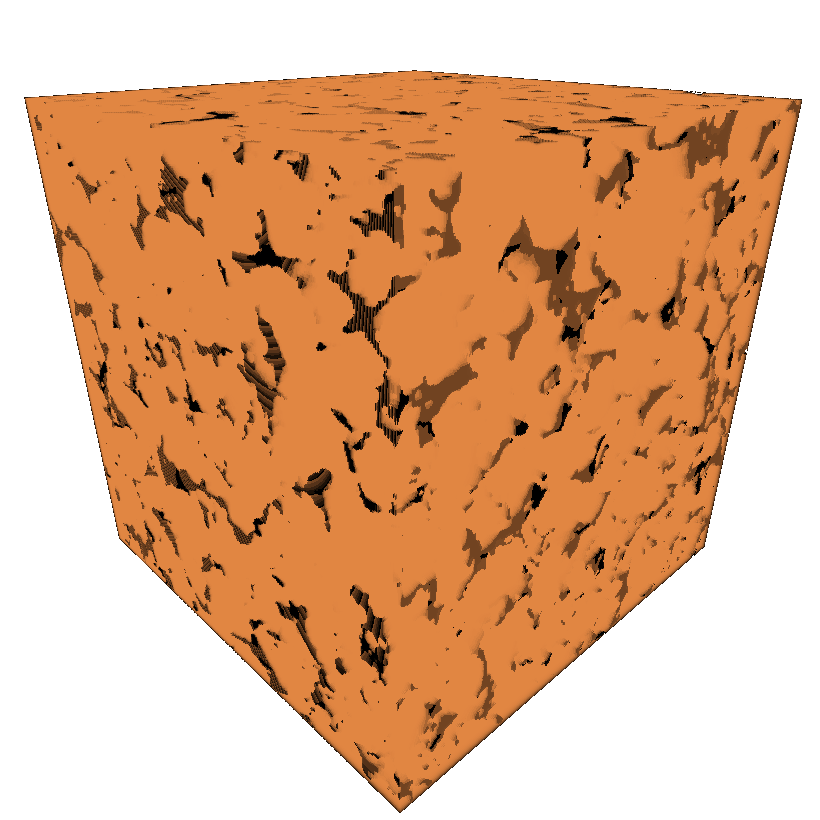
\includegraphics[width=0.3\linewidth]{images/sandstone3.png}
    \label{fig:sandstone3}}
  \vskip\baselineskip
  \subfigure[Carbonate 1, $C_{0.5} = 0.950$]{
    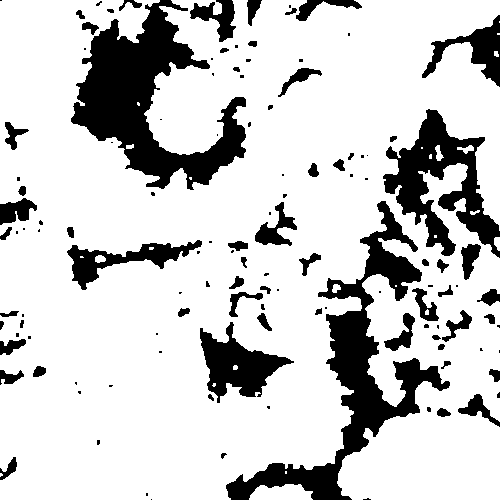
\includegraphics[width=0.3\linewidth]{images/carbonate1.png}
    \label{fig:carbonate1}}
  \hfill
  \subfigure[Carbonate 2, $C_{0.5} = 0.954$]{
    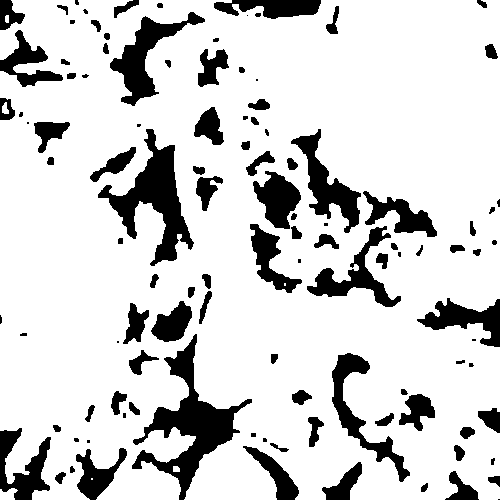
\includegraphics[width=0.3\linewidth]{images/carbonate2.png}
    \label{fig:carbonate2}}
  \hfill
  \subfigure[Carbonate 3, $C_{0.5} = 0.946$]{
    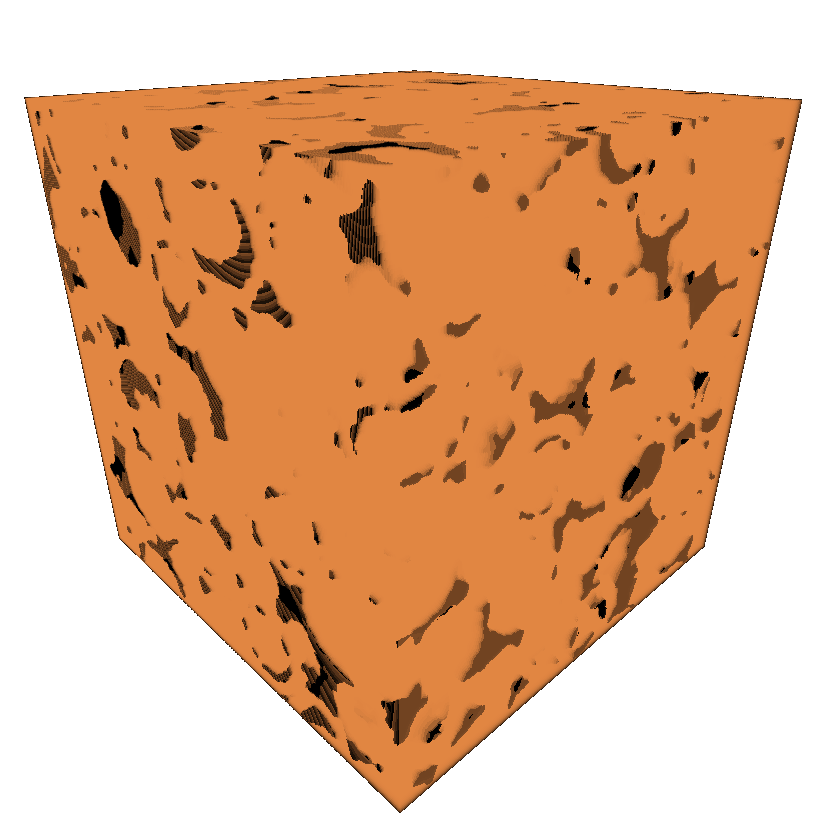
\includegraphics[width=0.3\linewidth]{images/carbonate3.png}
    \label{fig:carbonate3}}
  \caption[]{Data used in \cref{sec:application} for calculation of correlation
    functions.}
  \label{fig:real-data}
\end{figure*}

\begin{figure*}[t]
  \centering
  \subfigure[Surface-surface function]{
    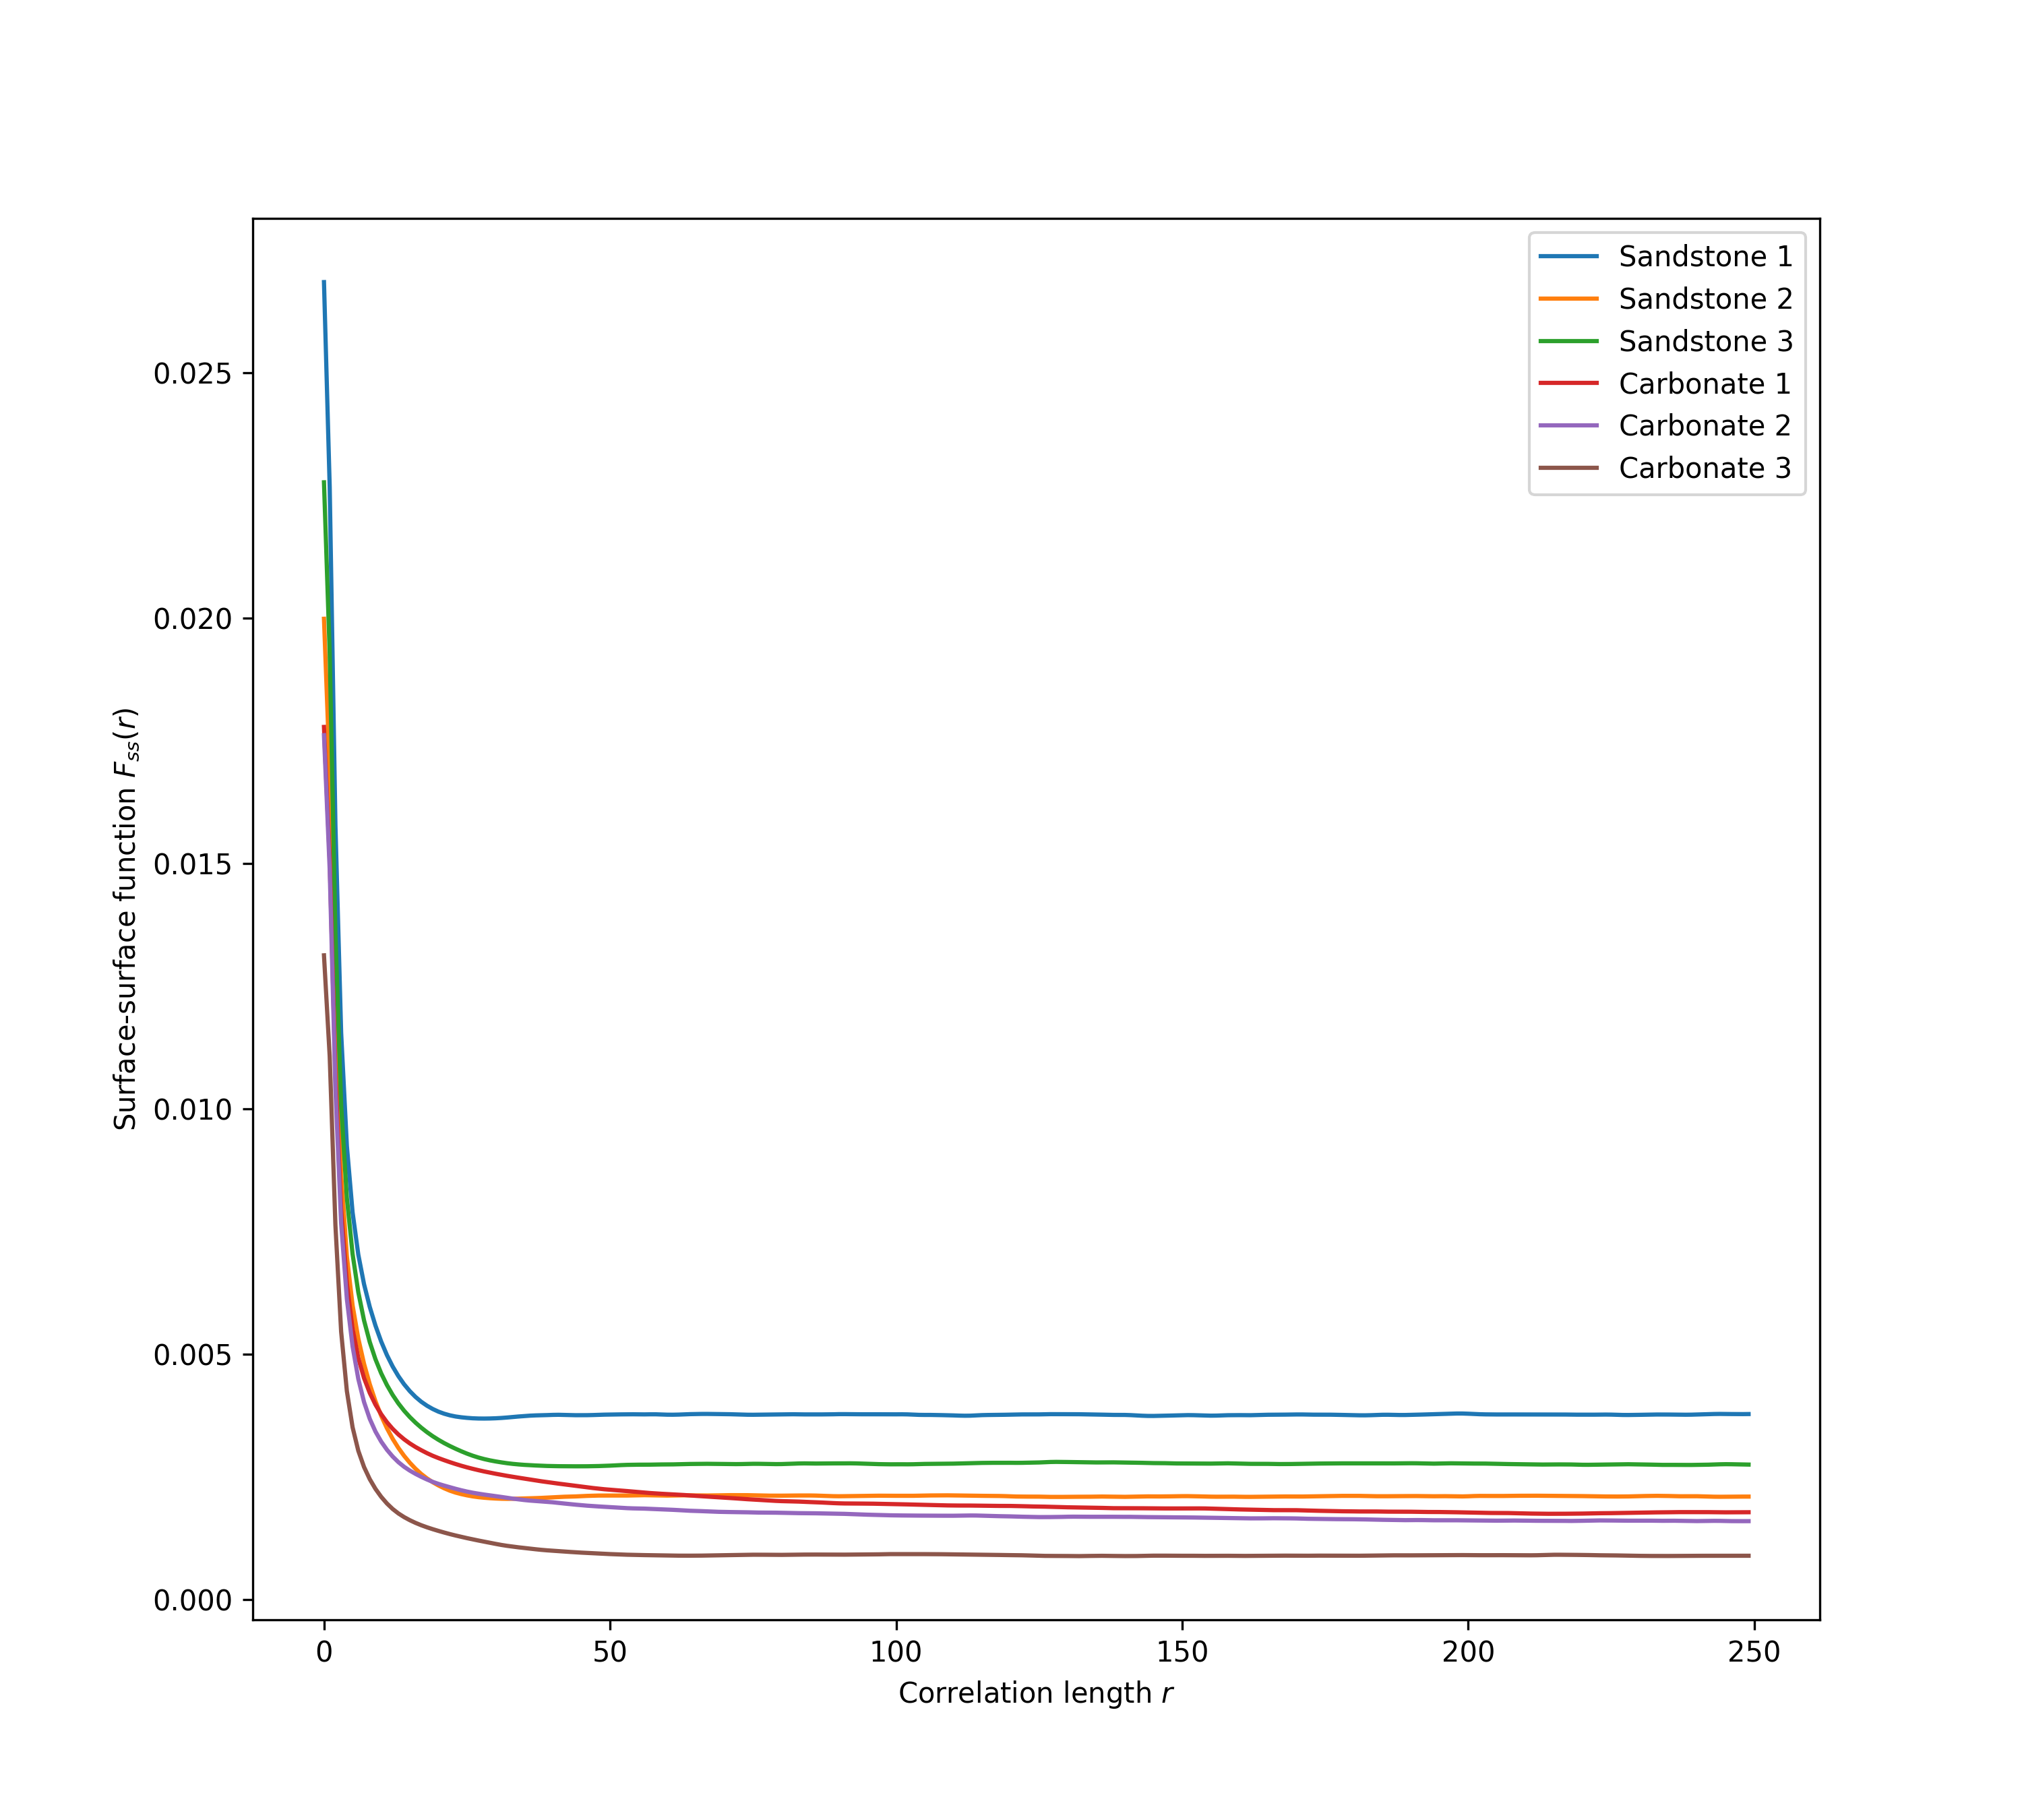
\includegraphics[width=0.475\linewidth]{images/KIK-ss.png}
    \label{fig:plot-ss-real}}
  \hfill
  \subfigure[Surface-void function]{
    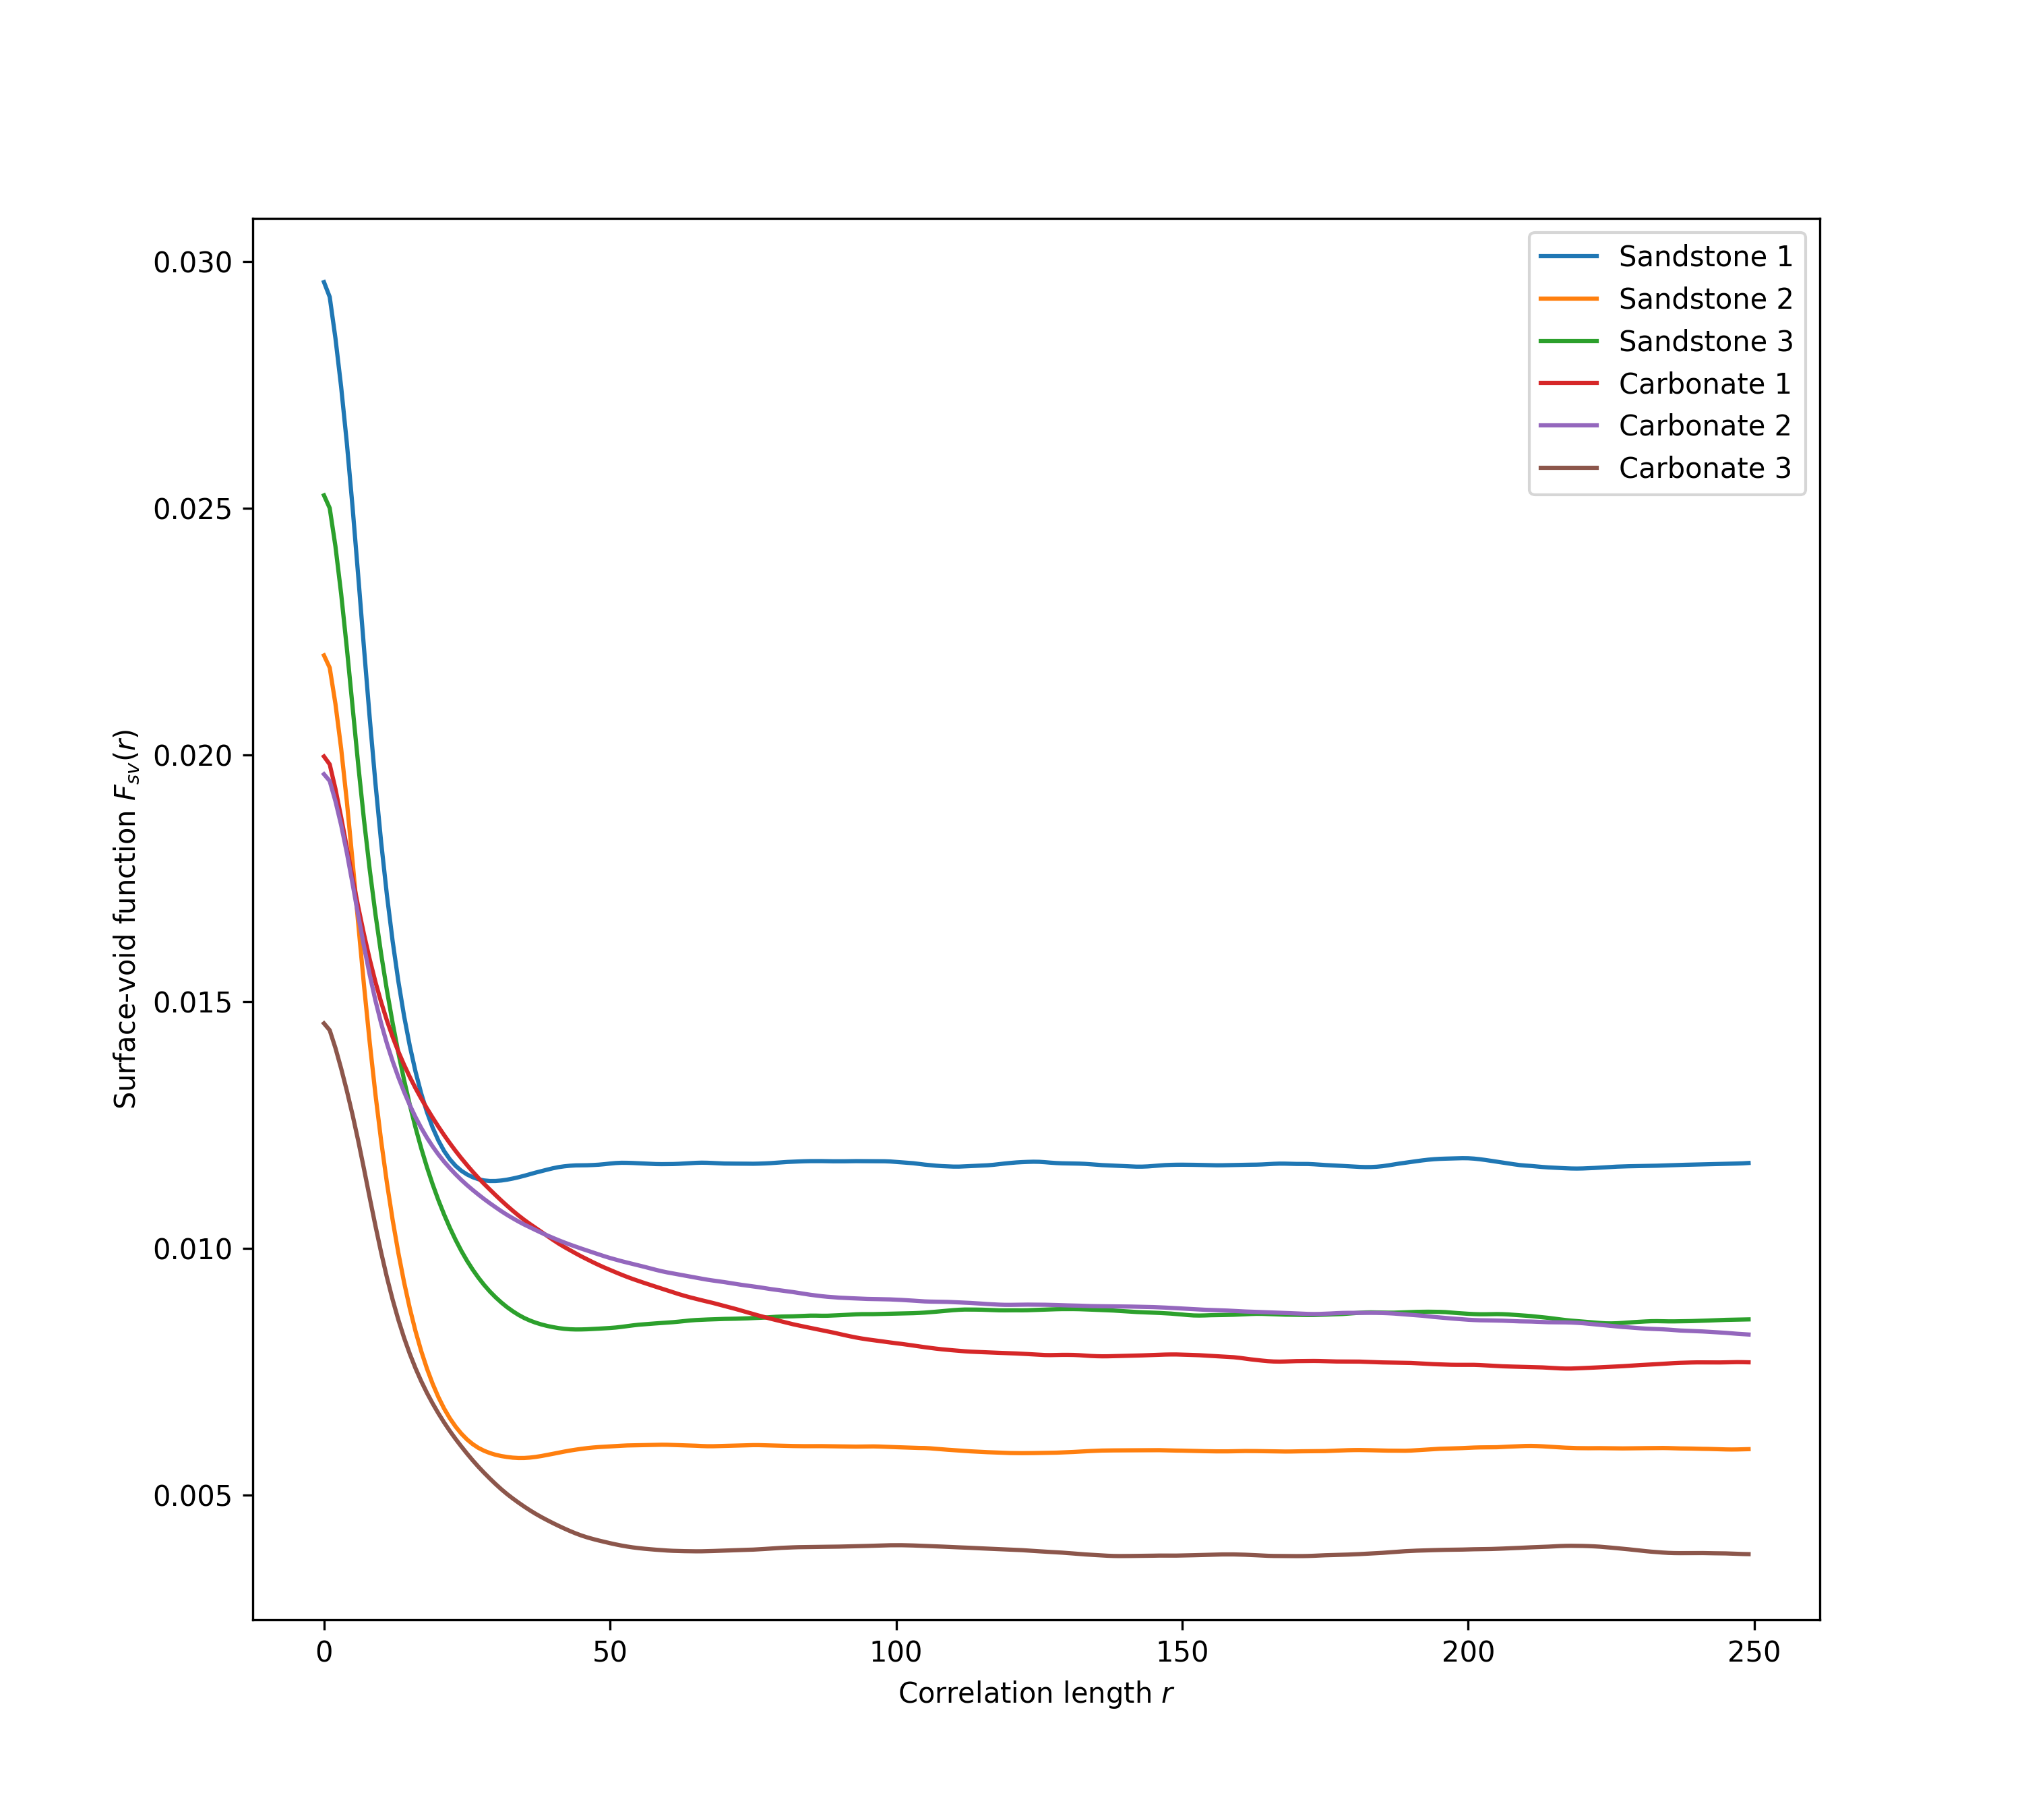
\includegraphics[width=0.475\linewidth]{images/KIK-sv.png}
    \label{fig:plot-sv-real}}
  \caption[]{Plots of $F_{ss}$ and $F_{sv}$ correlation functions computed for
    samples on \cref{fig:real-data}.}
  \label{fig:real-data-plots}
\end{figure*}

\begin{figure*}[t]
  \centering
  \subfigure[$C_{0.5} = 0.8397$]{
    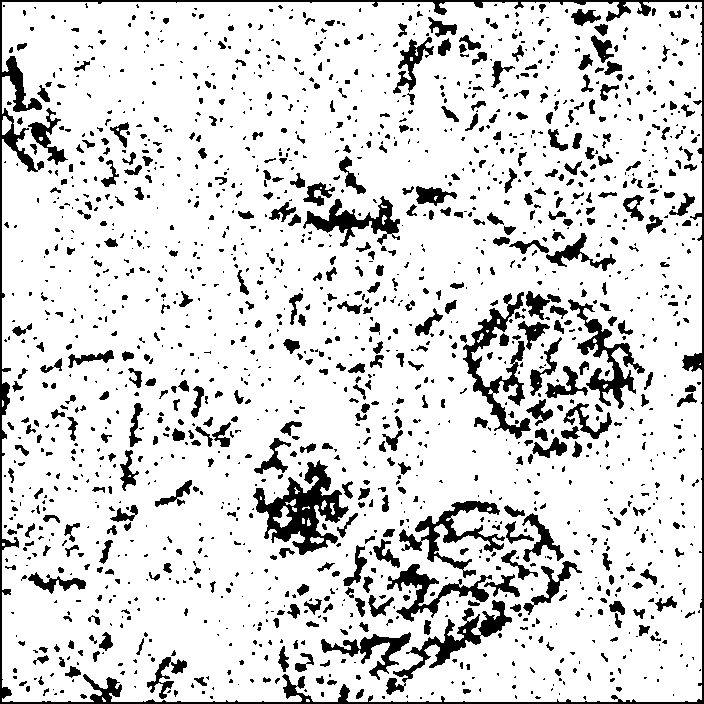
\includegraphics[width=0.475\linewidth]{images/sb-bad.png}
    \label{fig:bad1}}
  \hfill
  \subfigure[$C_{0.5} = 0.8517$]{
    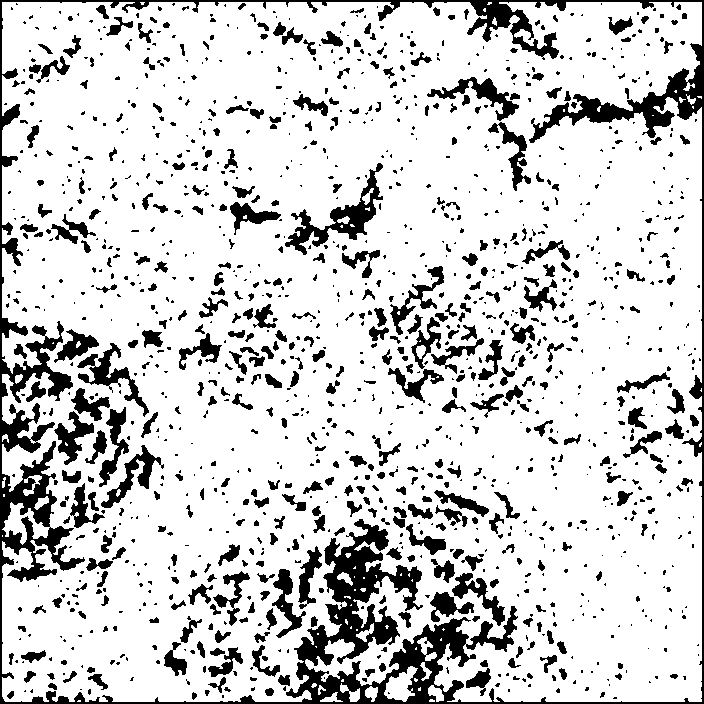
\includegraphics[width=0.475\linewidth]{images/sb-bad2.png}
    \label{fig:bad2}}
  \caption[]{Examples of images which do not pass $C_{0.5}$ criterion.}
  \label{fig:real-bad}
\end{figure*}

\section{Discussion and outline}
\label{sec:outline}
Exact vs. for-reconstruction computation of surface CFs

Our way it is easy to implement higher-order statistics computations, such as
multiple-point surface-surface correlation functions.

Discuss super-resolution to improve accuracy of surface functions computation
Explain that ``digital'' is better than ``continuous''.

\section{Conclusion}
\label{sec:summary}
Our summary says

\section{Acknowledgments}
This research was supported by the Russian Science Foundation grant
19-72-10082.

Collaborative effort of the authors within the FaT iMP (Flow and Transport in
Media with Pores) research group (www.porenetwork.com) and used some of its
software. We thank Prof. Salvatore Torquato for directing us to a
derivation of analytical formulas for 2D Poisson disks. Special thanks goes to
our colleague Dr. Dina Gafurova for the 2D and 3D images of real porous media
used in this study.

\appendix
\section{Derivation of analytical solutions for 2D Poisson disks}
\label{ap:overlapping-disks}
Analytic representation of surface-surface and surface-void correlation
functions for overlapping balls with centers generated by Poisson point process
is well known \cite{Torquato_book}:
\begin{align}
  F_{sv}(r) &= -\lim_{a_1 \rightarrow R} \frac{\partial}{\partial a_1}
  e^{-\lambda S_{tot}(r, a_1, R)} \label{eq:fsv-disks} \\
  F_{ss}(r) &= \lim_{a_1, a_2 \rightarrow R} \frac{\partial}{\partial a_1}
  \frac{\partial}{\partial a_2} e^{-\lambda S_{tot}(r, a_1,
    a_2)} \label{eq:fss-disks}
\end{align}
Here $S_{tot}(r, a_1, a_2)$ refers to a common volume of two n-dimensional balls
of radii $a_1$ and $a_2$ with a distance $r$ between their centers and $\lambda$
is a parameter of Poisson process. For two-dimensional disks we have the
following expression for $S_{tot}(r, a1, a2)$:
\begin{equation}
  S_{tot}(r, a_1, a_2) = \pi a_1^2 + \pi a_2^2 - S_{int}(r, a_1, a_2) \label{eq:total}
\end{equation}
where $S_{int}(r, a_1, a_2)$ is a common area of two disks, being equal to:
\begin{align}
  S_{int}(r, a_1, a_2) =&  a_1^2 \arccos(\frac{r^2+a_1^2-a_2^2}{2a_1r}) + \\
  & a_2^2 \arccos(\frac{r^2+a_2^2-a_1^2}{2a_2r}) - \\
  & \frac{\sqrt{Y}}{2} \label{eq:intersection}
\end{align}
when $r<2R$ and zero otherwise. $Y$ in \cref{eq:intersection} is
\begin{equation*}
  Y = (-r+a_1+a_2)(r+a_2-a_1)(r+a_1-a_2)(r+a_1+a_2)
\end{equation*}
Substituting \cref{eq:intersection} into \cref{eq:total} and then
\cref{eq:total} into \cref{eq:fss-disks} we obtain \cref{eq:fss_final} for
$F_{ss}(r)$.

Similarly substituting \cref{eq:intersection} into \cref{eq:total} and then
\cref{eq:total} into \cref{eq:fsv-disks} we obtain \cref{eq:fsv_final} for
$F_{sv}(r)$.

\section{Implementation of surface function computations}
The code used to compute surface correlation functions in this manuscript was
written in Julia language and available as a Jupyter notebook in Supplementary
Materials. It uses \code{CorrelationFunctions.jl} package developed by our group
\cite{CFsjlpaper} that allows efficient computation of surface and other
correlation functions using both CPU and GPU architectures.

\bibliography{apssamp}
\end{document}
